\documentclass[Lau,noexaminfo]{sapthesis}
\usepackage[italian]{babel}
\usepackage{url}
\usepackage[utf8]{inputenc}
\usepackage{hyperref}
\usepackage{textcomp}
\definecolor{gray}{gray}{0.4}
\usepackage{float}

\title{Modellazione di una macchina sincrona e controllo di tensione}
\author{Leonardo Salustri}
\IDnumber{1762556}
\course{Ingegneria Informatica e Automatica}
\courseorganizer{Facoltà di Ingegneria dell' Informazione, Informatica e Statistica}
\AcademicYear{2018/2019}
\copyyear{2019}
\advisor{Prof. Di Giorgio}
\tutor{Prof. Di Giorgio}
\schoolname{Liceo Blaise Pascal}
\schooladdress{Via Don Luigi Sturzo, Pomezia}
\authoremail{leo.salu97@gmail.com}

\begin{document}
	\frontmatter
	\maketitle
	
	\tableofcontents
	
	\setcounter{secnumdepth}{1}
	\setcounter{tocdepth}{1}
	\mainmatter
	\section*{Introduzione}
	L' obiettivo di questo lavoro è, una volta studiata la dinamica di una macchina sincrona, utilizzare il modello ottenuto in un contesto multimacchina, focalizzandosi sul controllo di tensione in un' analisi per piccoli segnali.
	Questa relazione verrà suddivisa fondamentalmente in tre capitoli: il primo riguarda lo studio della macchina sincrona isolata per arrivare a un modello con lo spazio di stato, il
	secondo riguarda l' inserimento della macchina in un contesto multi-macchina, mentre l' ultimo tratta lo studio del sistema di controllo della tensione, attraverso l' analisi dell' Automatic Voltage Regulator.
	Lo studio verrà effettuato su un modello linearizzato, poiché è di interesse lo studio della dinamica della rete controllata quando è soggetta a perturbazioni di piccola entità.
	Collocandoci nello studio della "small signal stability" ci si deve chiedere perché sia utile condurre questo tipo di analisi, che non tiene conto di variazioni di grande entità delle variabili che spesso si verificano nelle reti elettriche. Per rispondere bisogna avere chiara la struttura almeno superficiale di un power system.
	Questo è un sistema largamente interconnesso che ha il compito di trasportare e fornire ai nodi una certa quantità di potenza. Gli elementi fondamentali che costituiscono
	un sistema di potenza sono da una parte gli alternatori o macchine sincrone, che sono le sedi in cui viene prodotta l' energia elettrica, e un sistema di collegamenti
	che hanno il compito di trasportare tale energia. Un sistema del genere è molto vasto, spesso non è confinato in un solo paese, e proprio per la sua vastità e a causa di
	accorgimenti di tipo tecnologico un power system viene suddiviso in più sottosistemi. I collegamenti infatti possono far parte del sistema di trasmissione,
	o di quello di distribuzione. Il primo è l' insieme dei collegamenti che si occupano del trasporto, anche per lunghe distanze, dell' energia elettrica, mentre il secondo
	si occupa del dispaccio di energia nei centri più piccoli,per portare la corrente alle abitazioni o alle piccole industrie. La principale differenza tra i due sistemi
	è la tensione, poiché più è elevato il voltaggio meno perdite si hanno lungo la linea, soprattutto quando la linea elettrica percorre grandi distanze. Quindi una macchina
	sincrona che produce energia è sempre seguita da uno step-up transformer, che ha il compito di aumentare la tensione in ingresso secondo un certo rapporto di trasformazione.
	Questo implica che una volta che l' energia è arrivata al sistema di distribuzione, ci sia bisogno di un trasformatore che abbassi il livello di tensione, cosicché possa essere
	distribuita ai nodi finali.
	\begin{figure}
			\centering
			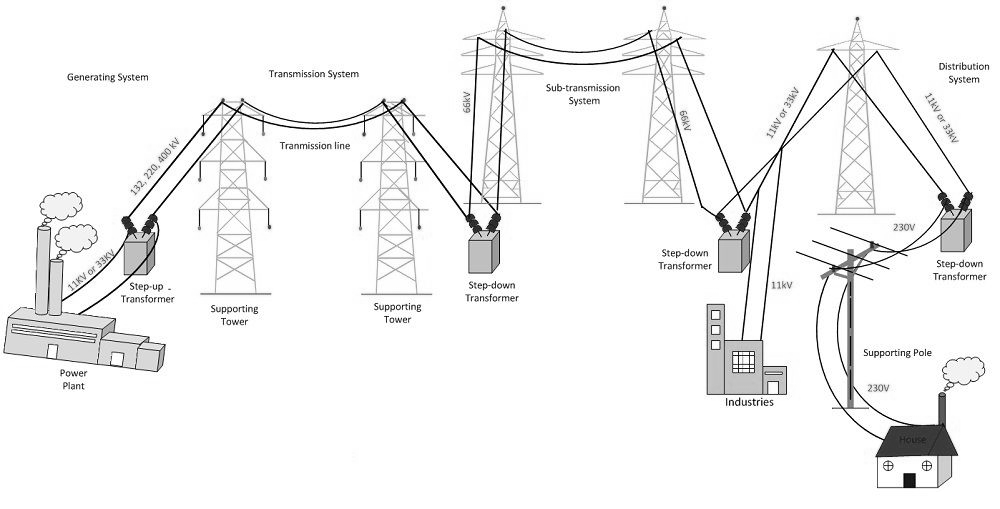
\includegraphics[height=0.450\textheight,angle=90]{trasmissione}
			\caption{Schema generale del trasporto di energia da origine a destinazione}
	\end{figure}
	In realtà come si può notare in figura 0.1 la situazione è più complessa, vi sono più sottoporzioni del power system, collegate le une alle altre attraverso altrettanti trasformatori.\\
	Avendo ora più chiaro il contesto in cui ci si pone possiamo capire come una variazione di domanda da parte di uno o più nodi presenti, nonostante l' impatto della
	variazione sia distribuito in un sistema così grande, abbia comunque un peso. Bisogna inoltre tener presente che per via della grande frequenza di variazione della domanda è difficile che un power system sia per molto tempo in equilibrio. E' proprio in questo preciso frangente che vuole 
	collocarsi questo studio, per studiare le oscillazioni delle variabili di interesse a seguito di piccole perturbazioni rispetto a un certo punto di lavoro, che è l' equilibrio 
	della rete.
	\chapter{}
	\section{Modellazione}
	\subsection{Descrizione e funzionamento}
	La macchina sincrona è costituita da due parti fisiche fondamentali: lo statore e il rotore.\\
	Il primo è un blocco cilindrico di metallo calettato in modo tale da poter posizionare i circuiti elettrici in direzione longitudinale. I conduttori costituiscono il cosiddetto circuito di armatura, composto dalle tre fasi sfasate di $\frac{2}{3}\pi$ l' una dall' altra.\\
	Per quanto riguarda il rotore invece vi è un' importante distinzione da fare a livello costruttivo. Esistono fondamentalmente due tipi di macchine, quelle a rotore liscio e quelle a poli salienti. In entrambi i casi il rotore è la parte rotante della macchina (da cui viene appunto il nome), e viene fatto ruotare grazie all' applicazione di una coppia meccanica da parte di una turbina. Nel primo tipo di alternatori il rotore è un grande blocco cilindrico di metallo, calettato come lo statore per poter alloggiare il circuito di field, cioè un circuito dove scorre corrente continua, e che viene alimentato da una struttura che prende il nome di sistema di eccitazione. Nel secondo tipo il rotore ha una forma ben più irregolare, poiché dalla parte centrale cilindrica vengono create delle protuberanze, i cosiddetti poli salienti. In questo secondo caso i circuiti di eccitazione possono essere molti di più, ciascuno avvolto trasversalmente su un polo, e la particolare forma finale delle espansioni polari viene costruita appositamente per rendere il campo magnetico che verrà prodotto nel traferro il più possibile simile a una forma sinusoidale.\\
	A livello di funzionamento la differenza tra le due soluzioni sta proprio nel tipo di energia primaria che viene usata per far ruotare il rotore. Nelle centrali termoelettriche, la coppia generata dalla turbina alimentata a vapore è abbastanza elevata da far girare il rotore a grandi velocità (3600 rpm), e di conseguenza le grandezze elettriche hanno frequenza pari a quella del rotore, come vedremo nei paragrafi successivi. Nelle centrali idroelettriche, al contrario, la coppia esercitata dalla turbina dipende dall' energia che il liquido fornisce alla stessa, che genera una rotazione del rotore con frequenza molto minore rispetto a quella generata dall' uso del vapore. Di conseguenza la frequenza delle grandezze elettriche sarebbe minore, inducendo così i progettisti ad aumentare i poli del rotore, così da ottenere frequenze elettriche pari a quelle delle macchine movimentate a vapore, a partire da una frequenza meccanica minore.
	\begin{figure}
		\centering
		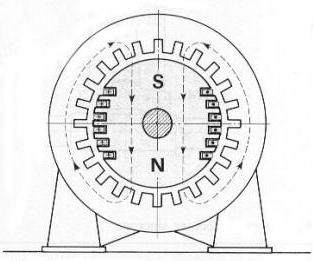
\includegraphics[scale=0.55]{poli_lisci1}
		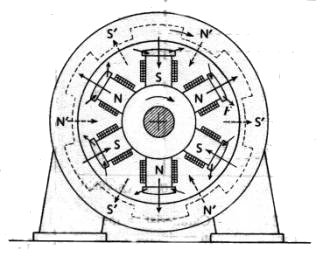
\includegraphics[scale=0.55]{poli_salienti1}
		\caption{Macchina sincrona con rotore a poli salienti a destra, e con rotore liscio a sinistra}
	\end{figure}
	Come possiamo vedere dalle figura 1.1 a sinistra troviamo un rotore liscio, con le calettature per il circuito di field, che produce una sola coppia polare, mentre a destra, sulla macchina a poli salienti troviamo 6 espansioni polari, con altrettanti avvolgimenti del circuito di rotore, e di conseguenza vi saranno tre coppie polari. Se chiamiamo $p$ il numero di coppie polari, che sono in rapporto uno a uno con le coppie di circuiti statorici per fase, la relazione che lega velocità angolare con la pulsazione delle grandezze elettriche è $\omega_r = \frac{\omega}{p}$, dove $\omega$ è la pulsazione delle grandezze elettriche e $\omega_r$ è la velocità angolare del rotore.\\
	Prima di ricavare le equazioni è utile definire una volta per tutte la struttura della macchina sincrona:\\
	1. Vi saranno tre circuiti monofase sullo statore sfasati tra loro di $\frac{2}{3}\pi$ (a,b,c);\\
	2. L' alternatore avrà un rotore liscio solido con il circuito di field avvolto in \\ \qquad direzione longitudinale (f);\\
	3. Verrà considerato un circuito di damping sul rotore (Q).\\
	Il circuito di damping sostanzialmente serve a livello modellistico a tener conto delle correnti parassite che scorrono nel blocco solido di metallo del rotore durante i transitori. Nelle macchine a poli salienti questi circuiti aggiuntivi vengono posizionati realmente sulla macchina per offrire appunto un passaggio a queste correnti parassite, mentre nelle macchine a rotore liscio vengono presi in considerazione nel modello proprio perché per propria natura questo tipo di rotore offre un passaggio alle correnti.
	\begin{figure}
		\centering
		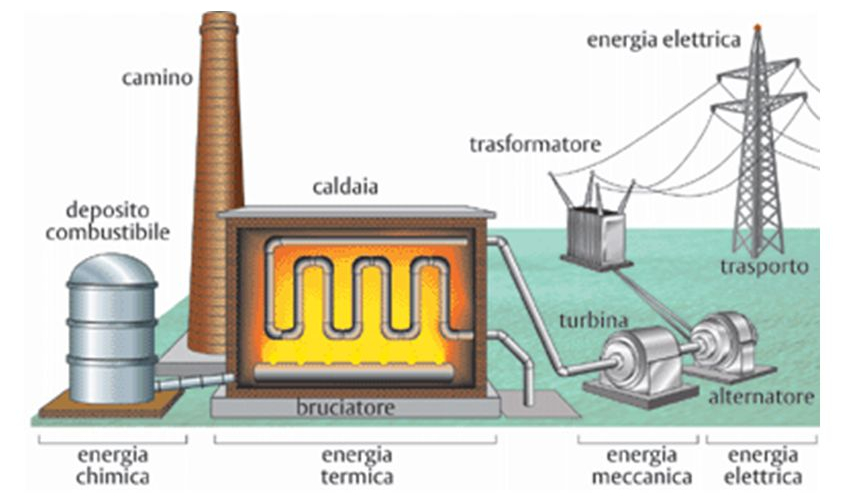
\includegraphics[height=0.3\textheight]{schema_generale}\\
		\caption{Schema generale centrale termoelettrica}
	\end{figure}
	Come si può notare figura 1.2 in una centrale termoelettrica viene creata energia termica attraverso l' impiego di combustibili, che successivamente viene trasformata in energia meccanica, ed attraverso la turbina viene applicata una coppia meccanica al rotore. Su quest' ultimo è presente il circuito di field, alimentato in continua esternamente dal sistema d' eccitazione, e viene prodotto un campo magnetico, il cui flusso concatenato con ciascuna delle tre fasi varierà nel tempo, poiché mentre le fasi sono in posizione fissa il campo magnetico è rotante a frequenza $f=\frac{\omega}{2\pi}$ (poiché viene generato dal circuito di field che ruota insieme al rotore). Questa variazione di flusso produrrà una forza elettromotrice nelle tre fasi, che in assenza di carico, non essendoci correnti e quindi cadute di tensione rimarrà fissa. Appena verrà collegato un carico ai terminali dei circuiti statorici nelle tre fasi scorreranno tre correnti, che nel caso il carico sia bilanciato, saranno una terna di correnti simmetriche e bilanciate. Queste genereranno a loro volta un campo magnetico di reazione (anch' esso "rotante"), che si sommerà con quello prodotto dal field, generando il campo magnetico risultante, che dipenderà quindi dal carico che è collegato alla macchina.
	\subsection{Derivazione del modello matematico}
	Come abbiamo detto le grandezze elettriche di cui vogliamo trovare le equazioni dinamiche sono delle grandezze che si riferiscono a tre fasi sfasate tra loro, e che quindi costituiscono una terna di un sistema trifase, di pulsazione $\omega$. Essendo difficile ragionare in questi termini, poiché si tratterà di maneggiare funzioni sinusoidali dipendenti dal tempo, per trattare le macchine elettriche di solito ci si sposta in un dominio diverso, quello di Park, che permette di eliminare la dipendenza dal tempo.
	\begin{figure}
	\centering
	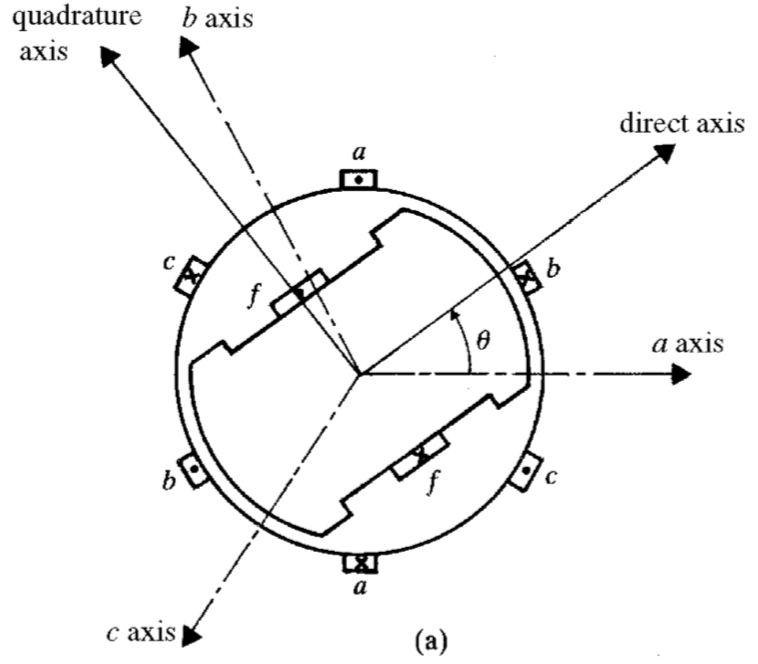
\includegraphics[height=0.30\textheight]{riferimento_park_pp}\\
	\caption{Riferimento nel dominio di Park}
	\end{figure}
	Sostanzialmente attraverso la trasformazione di Park ci si sposta in un riferimento rotante alla stessa velocità angolare del rotore, e che quindi ci permette di riferirci alle grandezze elettriche rotanti come grandezze fisse rispetto ai nuovi assi del sistema. Come possiamo vedere in figura 1.3 questi assi sono "diretta" (d), "quadratura" (q) e "omopolare" (o), dove l' ultimo non è visibile perché è in direzione perpendicolare agli altri due. Gli assi d e q sono sfasati tra loro di $\frac{\pi}{2}$. L' asse d, cioè quello di diretta, indica la direzione del vettore flusso del campo magnetico generato dal field, ed è proprio per questo che l' asse d funge da riferimento per il rotore: l' angolo individuato da quest' asse, rispetto alla direzione individuata dal flusso di campo magnetico concatenato con la fase A è detto "rotor angle" ed è pari a $\theta=\omega_r t+\delta $, dove il significato di $\delta$ sarà chiarito subito. E' stato già detto che se immaginiamo di trovarci in condizioni di carico collegato si genererà un campo magnetico di reazione che sommato al campo magnetico prodotto dal field darà luogo al campo magnetico risultante. L' angolo $\delta$ è proprio l' angolo che si individua tra il fasore del flusso del campo magnetico di field e il fasore del flusso del campo magnetico risultante. Questo angolo è detto load angle poiché appunto indica lo sfasamento che si ha tra i due flussi di campo proprio in relazione al carico che è collegato alla macchina. E' lo stesso angolo che si individua tra il fasore di tensione sullo statore e il fasore di tensione a vuoto. A livello intuitivo rappresenta lo sfasamento tra la tensione a vuoto e la tensione sullo statore per via della linea che connette la macchina alla sbarra. Quindi dipende dalle caratteristiche della linea, ma anche dalla corrente che vi scorre, che a sua volta dipende dal carico collegato.\\
	La matrice di trasformazione che ci consente di cambiare il nostro riferimento è:\\
	$P=\sqrt{\frac{2}{3}}\begin{bmatrix}
		\frac{1}{\sqrt2} & \frac{1}{\sqrt2} & \frac{1}{\sqrt2} \\
		\cos(\omega t) & \cos(\omega t -\frac{2}{3}\pi) & \cos(\omega t +\frac{2}{3}\pi) \\
		\sin(\omega t) & \sin(\omega t -\frac{2}{3}\pi) & \sin(\omega t +\frac{2}{3}\pi) \\
		
	\end{bmatrix}$\\
	E' una matrice ortogonale, quindi la sua inversa coincide con la trasposta.
	L' applicazione di questa matrice converte una terna trifase dipendente dal tempo in un vettore di tre componenti odq, rispettivamente omopolare, diretta e quadratura, che rispetto al nuovo sistema d' assi è indipendente dal tempo.\\
	Prendiamo ad esempio una terna di correnti simmetriche e bilanciate $I_{abc}$ e applichiamo la trasformazione:\\
	$I_{odq}=P I_{abc}=P \begin{bmatrix}
	I\cos(\omega t + \phi)\\
	I\cos(\omega t + \phi -\frac{2}{3}\pi) \\
	I\cos(\omega t + \phi +\frac{2}{3}\pi)
	\end{bmatrix}=
	\begin{bmatrix}
	0 \\
	\sqrt{\frac{3}{2}}I\cos(\phi)\\
	\sqrt{\frac{3}{2}}I\sin(\phi)
	\end{bmatrix}
	$\\
	E' da notare subito un' importante caratteristica della trasformazione, e cioè che se la terna trifase da trasformare è simmetrica e bilanciata la componente omopolare del vettore trasformato è sempre nulla. Quindi in una rete elettrica se la corrente omopolare è nulla si è sicuri che il carico che è agganciato alla rete è simmetrico e bilanciato.\newpage
	\paragraph{Equazioni dei flussi}Tenendo a mente la struttura dei circuiti della macchina possiamo scrivere:\\
	\[
	\begin{cases}
	\Psi_a=L_{aa} I_a + L_{ab} I_b +L_{ac} I_c + L_{af}I_f + L_{aQ} I_Q\\
	\Psi_b=L_{ba} I_a + L_{bb} I_b +L_{bc} I_c + L_{bf}I_f + L_{bQ} I_Q\\
	\Psi_c=L_{ca} I_a + L_{cb} I_b +L_{cc} I_c + L_{cf}I_f + L_{cQ} I_Q\\
	\Psi_f=L_{fa} I_a + L_{fb} I_b +L_{fc} I_c + L_{ff}I_f + L_{fQ} I_Q\\
	\Psi_Q=L_{Qa} I_a + L_{Qb} I_b +L_{Qc} I_c + L_{Qf}I_f + L_{QQ}I_Q\\
	\end{cases}
	\]\\
	dove $L_{ii}$ sono le autoinduttanze, di rotore o di statore, mentre $L_{ij}$ con $i \ne j$ sono mutue induttanze, tra una fase e un' altra, e tra i circuiti delle fasi e quelli del rotore.\\
	Andando a indagare sulle induttanze è facile intuire che esse hanno le seguenti caratteristiche:\\
	1. Le mutue induttanze tra le fasi dello statore hanno un valore fisso $M_s$, poiché i circuiti delle fasi sono fissi e quindi le loro induttanze non dipendono dal tempo;\\
	2. Le autoinduttanze delle fasi ($L_{aa},L_{bb},L_{cc}$) sono pari a $L_s$ che non dipende dal tempo;\\
	3. $L_{ff}$ e $L_{QQ}$, cioè le autoinduttanze dei circuiti rotorici sono fisse con un valore rispettivamente di $L_f$ e $L_Q$;\\
	4. Le mutue induttanze tra i circuiti rotorici sono nulle ($M_{fQ}=M_{Qf}=0$) poiché i circuiti sono ortogonali fra loro;\\
	5. Le mutue induttanze tra circuiti rotorici e le fasi dipendono dalla posizione del rotore, infatti:\\
	$L_{af} = M_f\cos(\omega t)=L_{fa}\\
	L_{bf}= M_f\cos(\omega t -\frac{2}{3}\pi)=L_{fb}\\
	L_{cf}= M_f\cos(\omega t +\frac{2}{3}\pi)=L_{fc}\\$
	$L_{aQ} = M_Q\cos(\omega t)=L_{Qa}\\
	L_{bQ}= M_Q\cos(\omega t -\frac{2}{3}\pi)=L_{Qb}\\
	L_{cQ}= M_Q\cos(\omega t +\frac{2}{3}\pi)=L_{Qc}\\$
	  Possiamo quindi riscrivere tutto in maniera più compatta:\\
	$\begin{bmatrix}
		\Psi_a\\
		\Psi_b\\
		\Psi_c\\
		\Psi_f\\
		\Psi_Q
	\end{bmatrix}=
	\begin{bmatrix}
		L_s & -M_s & -M_s & L_{af} & L_{aQ}\\
		-M_s & L_s & -M_s & L_{bf} & L_{bQ}\\
		-M_s & -M_s & L_s & L_{cf} & L_{cQ}\\
		L_{fa} & L_{fb} & L_{fc} & L_f & 0\\
		L_{aQ} & L_{bQ} & L_{cQ} & 0 & L_Q
	\end{bmatrix}
	\begin{bmatrix}
		I_a\\
		I_b\\
		I_c\\
		I_f\\
		I_Q
	\end{bmatrix}$\\\\\\
	Per effettuare la trasformazione di Park delle equazioni dei flussi è più conveniente scrivere tutto nella forma:\\\\
	$\begin{bmatrix}
	\Psi_{abc}\\
	\Psi_{fQ}\\
	\end{bmatrix}=
	\begin{bmatrix}
	L_{ss} & L_{sr}\\
	L_{rs} & L_{rr}
	\end{bmatrix}
	\begin{bmatrix}
	I_{abc}\\
	I_{fQ}\\
	\end{bmatrix}$ \\\\
	dove $L_{sr}$ e $L_{rs}$ sono matrici delle induttanze statore-rotore e rotore-statore, $L_{ss}$ è la matrice delle induttanze statore-statore, e $L_{rr}$ è la matrice delle induttanze rotore-rotore. \\Allora possiamo scrivere:\\\\
	$\begin{bmatrix}
	P & 0\\
	0 & I
	\end{bmatrix}\begin{bmatrix}
		\Psi_{abc}\\
		\Psi_{fQ}\\
	\end{bmatrix}=
	\begin{bmatrix}
		P & 0\\
		0 & I
	\end{bmatrix}
	\begin{bmatrix}
	L_{ss} & L_{sr}\\
	L_{rs} & L_{rr}
	\end{bmatrix}
	\begin{bmatrix}
	P^{-1} & 0\\
	0 & I
	\end{bmatrix}
	\begin{bmatrix}
	P & 0\\
	0 & I
	\end{bmatrix}
	\begin{bmatrix}
	I_{abc}\\
	I_{fQ}\\
	\end{bmatrix}$\\\\
	Infine quindi si arriva a scrivere che:\\\\
	\begin{equation}
	\begin{bmatrix}
		\Psi_o\\
		\Psi_d\\
		\Psi_q\\
		\Psi_f\\
		\Psi_Q
	\end{bmatrix}=
	\begin{bmatrix}
	L_o & 0 & 0 & 0 & 0\\
	0 & L_d & 0 & kM_f & 0\\
	0 & 0 & L_q & 0 & kM_Q\\
	0 & kM_f & 0 & L_f & 0\\
	0 & 0 & kM_Q & 0 & L_Q
	\end{bmatrix}
	\begin{bmatrix}
	I_o\\
	I_d\\
	I_q\\
	I_f\\
	I_Q
	\end{bmatrix}\\
	\end{equation}
	dove $L_o=L_s - 2M_s$, $L_d=L_q=L_s+M_s$, $k=\sqrt{\frac{3}{2}}$.
	\paragraph{Equazioni delle tensioni}
	Per trovare le equazioni delle tensioni risulta più semplice analizzare i circuiti equivalenti delle tre fasi e dei circuiti sul rotore, che sono riportati in figura 1.4.
	\begin{figure}
		\centering
		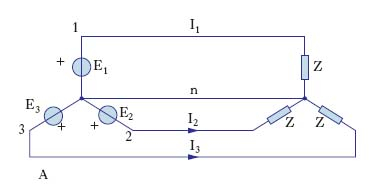
\includegraphics[height=0.3\textheight]{trifase}\\
		\caption{Circuiti equivalenti delle tre fasi e dei circuiti rotorici}
	\end{figure}
	Adottando la convenzione dei generatori, quindi con le correnti che scorrono dalla macchina verso la rete, possiamo scrivere:\\
	$V-V_n=-rI-\dot{\Psi}$, \\e questa equazione vale per tutte e tre le fasi dello statore. $V_n$ è la tensione di neutro ed è diversa da zero solo se la somma delle correnti nelle fasi è diversa da zero, cioè se il carico non è bilanciato.\\
	Per il circuito di field invece adottiamo la condizione di carico, poiché questo è alimentato dal sistema di eccitazione e quindi:\\
	$V_f=r_fI_f+\dot{\Psi}_f$.\\
	Per quanto riguarda il circuito di damping, esso è cortocircuitato poiché non vi è una tensione vera e propria che determina lo scorrimento di corrente, infatti quest' ultima vi scorre solo nei transitori, quindi:\\
	$V_Q=0=r_QI_Q + \dot{\Psi}_Q$.\\Scrivendo tutto in forma matriciale abbiamo\\\\
	$\begin{bmatrix}
		V_a\\
		V_b\\
		V_c\\
		-V_f\\
		0
	\end{bmatrix}=-
	\begin{bmatrix}
		r_a & 0 & 0 & 0 & 0\\
		0 & r_b & 0 & 0 & 0\\
		0 & 0 & r_c & 0 & 0\\
		0 & 0 & 0 & r_f & 0\\
		0 & 0 & 0 & 0 & r_Q\\
	\end{bmatrix}
	\begin{bmatrix}
		I_a\\
		I_b\\
		I_c\\
		I_f\\
		I_Q
	\end{bmatrix}-
	\begin{bmatrix}
		\dot{\Psi}_a\\
		\dot{\Psi}_b\\
		\dot{\Psi}_c\\
		\dot{\Psi}_f\\
		\dot{\Psi}_Q
	\end{bmatrix} +
	\begin{bmatrix}
		V_n\\
		0\\
		0
	\end{bmatrix}$,\\
	dove $V_n=-r_n
	\begin{bmatrix}
	 1 & 1 & 1\\
	 1 & 1 & 1\\
	 1 & 1 & 1
	\end{bmatrix}
	\begin{bmatrix}
	I_a\\
	I_b\\
	I_c
	\end{bmatrix}-
	L_n
	\begin{bmatrix}
	1 & 1 & 1\\
	1 & 1 & 1\\
	1 & 1 & 1
	\end{bmatrix}
	\begin{bmatrix}
	\dot{I}_a\\
	\dot{I}_b\\
	\dot{I}_c
	\end{bmatrix}$\\\\
	Per effettuare la trasformazione nel dominio di Park conviene scrivere le equazioni in maniera sintetica:\\
	$\begin{bmatrix}
		V_{abc}\\
		V_{fQ}
	\end{bmatrix}=-
	\begin{bmatrix}
		R_{abc} & 0\\
		0 & R_{fQ}
	\end{bmatrix}
	\begin{bmatrix}
	I_{abc}\\
	I_{fQ}
	\end{bmatrix}-
	\begin{bmatrix}
	\dot{\Psi}_{abc}\\
	\dot{\Psi}_{fQ}
	\end{bmatrix}+
	\begin{bmatrix}
	V_{n}\\
	0
	\end{bmatrix}$, dove si ricordi che\\
	$V_{fQ}=\begin{bmatrix}
	-V_{f}\\
	0
	\end{bmatrix}$.\\ La trasformazione di Park questa volta verrà fatta elemento dopo elemento perché i termini con derivata temporale complicheranno la scrittura. Esaminando la partizione dei vettori in due gruppi, quello delle tre fasi e quello dei circuiti sul rotore possiamo effettuare la trasformazione usando la matrice $\begin{bmatrix}
	P & 0\\
	0 & I_3
	\end{bmatrix}$, dove $I_3$ è la matrice Identità di dimensoni 3x3.\\\\
	1. \textbf{Tensioni}\\\\
	$\begin{bmatrix}
	P & 0\\
	0 & I_3
	\end{bmatrix}
	\begin{bmatrix}
		V_{abc}\\
		V_{fQ}
	\end{bmatrix}=
	\begin{bmatrix}
		V_{odq}\\
		V_{fQ}
	\end{bmatrix}$\\\\\\
	2. \textbf{Caduta tensione sulle resistenze}\\\\
	$\begin{bmatrix}
	P & 0\\
	0 & I_3
	\end{bmatrix}
	\begin{bmatrix}
	r_{abc} & 0\\
	0 & r_{fQ} 
	\end{bmatrix}
	\begin{bmatrix}
	I_{abc}\\
	I_{fQ}
	\end{bmatrix}=
	\begin{bmatrix}
		P & 0\\
		0 & I_3
	\end{bmatrix}
	\begin{bmatrix}
		r_{abc} & 0\\
		0 & r_{fQ}
	\end{bmatrix}
	\begin{bmatrix}
	P^{-1} & 0\\
	0 & I_3
	\end{bmatrix}
	\begin{bmatrix}
	P & 0\\
	0 & I_3
	\end{bmatrix}
	\begin{bmatrix}
		I_{abc}\\
		I_{fQ}
	\end{bmatrix}=\\
	\begin{bmatrix}
	P & 0\\
	0 & I_3
	\end{bmatrix}
	\begin{bmatrix}
	r_{abc} & 0\\
	0 & r_{fQ}
	\end{bmatrix}
	\begin{bmatrix}
	P^{-1} & 0\\
	0 & I_3
	\end{bmatrix}
	\begin{bmatrix}
	I_{odq}\\
	I_{fQ}
	\end{bmatrix}=
	\begin{bmatrix}
	Pr_{abc}P^{-1} & 0\\
	0 & r_{fQ}
	\end{bmatrix}
	\begin{bmatrix}
	I_{odq}\\
	I_{fQ}
	\end{bmatrix}=
	\begin{bmatrix}
		r_{abc} & 0\\
		0 & r_{fQ}
	\end{bmatrix}
	\begin{bmatrix}
	I_{odq}\\
	I_{fQ}
	\end{bmatrix}$\\\\\\
	3. \textbf{Caduta di tensione sulle induttanze}\\\\
	$\begin{bmatrix}
	P & 0\\
	0 & I_3
	\end{bmatrix}
	\begin{bmatrix}
	\dot{\Psi}_{abc}\\
	\dot{\Psi}_{fQ}
	\end{bmatrix}=
	\begin{bmatrix}
	P \dot{\Psi}_{abc}\\
	\dot{\Psi}_{fQ}
	\end{bmatrix}$. \\\\
	Per calcolare $P \dot{\Psi}_{abc}$ si ricordi che $\Psi_{odq}=P\Psi_{abc}$, quindi $\dot{\Psi}_{odq}=\dot{P}\Psi_{abc} + P\dot{\Psi}_{abc}$, e $P\dot{\Psi}_{abc}=\dot{\Psi}_{odq}-\dot{P}\Psi_{abc}=\dot{\Psi}_{odq} - \dot{P}P^{-1}\Psi_{odq}$\\\\\\
	$\dot{P}P^{-1}=\omega
	\begin{bmatrix}
		0 & 0 & 0\\
		0 & 0 & -1\\
		0 & 1 & 0
	\end{bmatrix}$ quindi:\\
	$P\dot{\Psi}_{abc}=\dot{\Psi}_{odq} - \omega
	\begin{bmatrix}
	0 & 0 & 0\\
	0 & 0 & -1\\
	0 & 1 & 0
	\end{bmatrix}\Psi_{odq}$\\\\\\\\
	4. \textbf{Tensione di neutro}\\\\
	$\begin{bmatrix}
	P & 0\\
	0 & I_2
	\end{bmatrix}
	\begin{bmatrix}
		V_n\\
		0
	\end{bmatrix}=
	\begin{bmatrix}
	PV_n\\
	0
	\end{bmatrix},\\
	PV_n=-PR_nP^{-1}I_{odq}-PL_nP^{-1}I_{odq}=
	\begin{bmatrix}
		-3r_nI_o-3L_n\dot{I_o}\\
		0\\
		0\\
	\end{bmatrix}$\\\\
	Quindi possiamo scrivere\\
	\begin{equation}
	\begin{bmatrix}
	V_{odq}\\
	V_{fQ}
	\end{bmatrix}=
	\begin{bmatrix}
	r_{abc} & 0\\
	0 & r_{fQ}
	\end{bmatrix}
	\begin{bmatrix}
	I_{odq}\\
	I_{fQ}
	\end{bmatrix}-
	\begin{bmatrix}
	\dot{\Psi}_{odq}\\
	\dot{\Psi}_{fQ}
	\end{bmatrix}+
	\begin{bmatrix}
	\dot{P}P^{-1}\Psi_{odq}\\
	0
	\end{bmatrix}+
	\begin{bmatrix}
	PV_n\\
	0
	\end{bmatrix}
	\end{equation}\\\\
	Si tenga presente che nel caso di carico bilanciato, data la simmetria del sistema, si eliminerà ogni contributo della corrente omopolare, quindi anche l' ultimo termine del membro di destra dell' equazione delle tensioni.
	\paragraph{Equazione della coppia}
	Prima di procedere con la determinazione del modello con lo spazio di stato occorre esaminare la dinamica del rotore, che permette di collegare la parte elettrica della macchina a quella meccanica. La potenza delle tre fasi è data da:\\
	$V_a I_a + V_b I_b + V_c I_c = V^T_{abc} I_{abc}=(P^{-1}V_{odq})^T P^{-1}I_{odq}=V_{odq}^T P P^{-1} I_{odq}=V_{odq}^T I_{odq}$. Da questa relazione si capisce, per quanto riguarda la potenza, come il prodotto tensioni-correnti viene conservato nel dominio di Park. Utilizzando le equazioni delle tensioni possiamo sostituire le tensioni con espressioni che sono funzioni delle correnti. Assumeremo un carico bilanciato, quindi lavoreremo sull' equazione\\
	$P=V_{dq}^T I_{dq}$.\\
	$P=V_{dq}^T I_{dq}=-r(I_d^2+I_q^2) + \omega(L_d I_dI_q +kM_QI_dI_Q+kM_f I_qI_f-L_qI_dI_q) -kM_f I_d \dot{I}_f -L_qI_q \dot{I}_q - L_dI_d\dot{I}_d -kM_QI_q\dot{I}_Q$.\\
	Il membro di destra è composto da tre gruppi fondamentali, che sono stati raggruppati in parentesi, che esaminiamo da sinistra verso destra:\\
	1. La potenza dissipata sulle resistenze dei circuiti statorici;\\
	2. La potenza elettrica, che è di nostro grande interesse, poiché esprime l' accoppiamento naturale che esiste tra la parte elettrica e la parte meccanica della macchina sincrona. Infatti questo accoppiamento è dato dalla presenza di $\omega$ nell' espressione. Difatti:\\
	$C_e=\frac{\partial P}{\partial \omega} = L_dI_dI_q+kM_QI_dI_Q+kM_fI_qI_f-L_qI_dI_q $, dove $C_e$ è la coppia elettrica.\\
	3. La potenza utilizzata per i flussi del campo magnetico, riconoscibile per la presenza delle derivate, infatti osservando di nuovo la figura 1.4 questo termine coincide con la potenza dissipata sulle induttanze.\\\\
	La coppia elettrica (che è stata indicata come $C_e$) va a comporre una parte fondamentale della dinamica del rotore, in quanto è una coppia derivante dall' azione del carico agganciato alla macchina che va ad agire direttamente sulla velocità angolare del rotore. La quinta equazione differenziale di cui abbiamo bisogno è proprio quella che descrive la dinamica della $\omega$ del rotore, e per un corpo rigido rotante vale:\\
	\begin{equation}
	J\dot{\omega}=C_m - D\omega - C_e 
	\end{equation} dove $C_m$ è la coppia meccanica esercitata dalla turbina e $D\omega$ è una coppia resistente dovuta ad attriti interni, che però non è sempre lecito trascurare, poiché spesso si preferisce rappresentare in maniera meno specifica la parte elettrica della macchina eliminando i circuiti di damping e inglobando il loro effetto in un aumento del coefficiente D.
	\paragraph{Equazione della dinamica del load angle}
	Nell' analisi di una macchina sincrona collegata a un carico, dove quest' ultimo può anche essere immaginato come una vera e propria rete, gioca un ruolo importante il load angle. E' stato già detto che il riferimento per la misura degli angoli è posto lungo la direzione del vettore di flusso del campo magnetico attraverso la fase A della macchina. E' noto che tutte le grandezze elettriche della macchina possono essere rappresentate come dei vettori rotanti di velocità angolare $\omega$. All' istante t=0 il vettore rotante della tensione di statore $\bar{V}$ si trova proprio allineato con il riferimento, e di conseguenza l' angolo che si individua tra il vettore rotante $\bar{E}$ e $\bar{V}$ è proprio il load angle $\delta$.\\
	In linea generale il load angle è quell' angolo di sfasamento che si ha tra il fasore di tensione a vuoto ($\bar{E}$), che si trova sempre lungo l' asse di quadratura, e il fasore di tensione con carico agganciato ($\bar{V}$). Se noi immaginiamo la rete a regime questi vettori sono tutti rotanti alla stessa velocità angolare, quindi non appena si verifica un transitorio, il fasore di tensione a vuoto $\bar{E}$ rimane fisso rispetto al riferimento, mentre $\bar{V}$ verrà sfasato e quindi $\delta$ varierà. Con la sua variazione, varieranno anche le proiezioni di $\bar{V}$ lungo d e q, quindi varieranno $V_d$ e $V_q$. E' proprio per questo che è importante determinare la dinamica di questo angolo, che per quanto detto è influenzata dalla velocità angolare del rotore della macchina:\\
	\begin{equation}
	\dot{\delta}=\omega-\Omega_{rif}
	\end{equation}
	dove $\Omega_{rif}$ è la velocità angolare di riferimento, cioè quella di regime.
	
	\subsection{Modello con lo spazio di stato}Per determinare il modello con lo spazio di stato si utilizzeranno proprio le equazioni (1.2) e vi si aggiungeranno le due equazioni differenziali (1.3) e (1.4). La scelta principale è quella che riguarda le variabili di stato. Possono essere scelti i flussi come variabili, o le correnti, e in questo lavoro si prenderà in considerazione un modello in correnti. Esaminando le equazioni delle tensioni bisogna utilizzare le relazioni tra flussi e correnti (1.1) per far scomparire i primi dal modello. Dopo vari passaggi e immaginando di avere un carico bilanciato, quindi considerando pari a zero la corrente omopolare, si ottiene:
	\begin{equation*}
	\resizebox{0.98\hsize}{!}{%
		$\begin{bmatrix}
		V_d \\
		-V_f \\
		V_q \\
		V_Q=0
		\end{bmatrix}=
		-\begin{bmatrix}
		r & 0 & \omega L_q & \omega kM_Q \\
		0 & r_f & 0 & 0\\
		-\omega L_d & -\omega kM_f & r & 0\\
		0 & 0 & 0 & r_Q
		\end{bmatrix}
		\begin{bmatrix}
		I_d\\
		I_f\\
		I_q\\
		I_Q
		\end{bmatrix}
		-\begin{bmatrix}
		L_d & kM_f & 0 & 0\\
		kM_f & L_f & 0 & 0\\
		0 & 0 & L_q &  kM_Q\\
		0 & 0 & kM_Q & L_Q
		\end{bmatrix} \begin{bmatrix}
		\dot{I}_d\\
		\dot{I}_f\\
		\dot{I}_q\\
		\dot{I}_Q
		\end{bmatrix} $
	}
	\end{equation*}
	Come vediamo queste equazioni sono della forma\\
	$V_{dfqQ}=-H I_{dfqQ} - G \dot{I}_{dfqQ}$, \\quindi lo spazio di stato sarà della forma:\\
	$\dot{I}_{dfqQ}= -G^{-1}H I_{dfqQ} - G^{-1}V_{dfqQ} $.\\
	Quindi dopo aver invertito la matrice ed aver effettuato pochi passaggi, avendo aggiunto le due ulteriori equazioni differenziali (1.3) e (1.4), avremo:\\\\
	$\begin{bmatrix}
	\dot{I}_d \\
	\dot{I}_f \\
	\dot{I}_q \\
	\dot{I}_Q \\
	J\dot{\omega}\\
	\dot{\delta}\\
	\end{bmatrix}=-
	\begin{bmatrix}
	\frac{L_f r}{k^2 M_f^2-L_d L_f} & \frac{kM_f r_f}{k^2M_f^2 - L_dL_f} & \frac{-L_f L_q \omega}{k^2 M_f^2 - L_d L_f} & \frac{-Lf kM_q \omega}{k^2 M_f^2 - L_d L_f} & 0 & 0\\
	\frac{kM_f r}{k^2 M_f^2-L_d L_f} & \frac{-L_d r_f}{k^2M_f^2 - L_dL_f} & \frac{kM_f \omega L_q}{k^2 M_f^2 - L_d L_f} & \frac{k^2M_fM_Q \omega}{k^2 M_f^2 - L_d L_f} & 0 & 0\\
	\frac{\omega L_d L_Q}{k^2 M_Q^2 -L_q L_Q} & \frac{kM_f L_Q \omega}{k^2 M_Q^2 -L_q L_Q} & \frac{-L_Q r}{k^2 M_Q^2 -L_q L_Q} & \frac{k r_Q M_Q}{k^2 M_Q^2 -L_q L_Q} & 0 & 0\\
	\frac{-L_d M_Q k \omega}{k^2 M_Q^2 -L_q L_Q} & \frac{-M_f M_Q k^2 \omega}{k^2 M_Q^2 -L_q L_Q} & \frac{kM_Q r}{k^2 M_Q^2 -L_q L_Q} & \frac{-L_q r_Q}{k^2 M_Q^2 -L_q L_Q} & 0 & 0\\
	L_d I_q & kM_f I_q & -L_q I_d & -kM_QI_d & D & 0 \\
	0 & 0 & 0 & 0 & -1 &0 
	
	\end{bmatrix}
	\begin{bmatrix}
	I_d \\
	I_f \\
	I_q \\
	I_Q\\
	\omega\\
	\delta
	\end{bmatrix}-\newline
	\begin{bmatrix}
	\frac{-L_f}{k^2 M_f^2-L_d L_f} & \frac{kM_f}{k^2 M_f^2-L_d L_f} & 0 & 0 & 0 & 0 \\
	\frac{kM_f}{k^2 M_f^2-L_d L_f} & \frac{-L_d}{k^2 M_f^2-L_d L_f} & 0 &0 & 0 & 0\\
	0 & 0 & \frac{-L_Q}{k^2 M_Q^2 -L_q L_Q} & \frac{kM_Q}{k^2 M_Q^2 -L_q L_Q} & 0 & 0\\
	0 & 0 &  \frac{kM_Q}{k^2 M_Q^2 -L_q L_Q} & - \frac{-L_Q}{k^2 M_Q^2 -L_q L_Q} & 0 &0 \\
	0 & 0 & 0 & 0 & -1 & 0 \\
	0 & 0 & 0 & 0 & 0 & 1
	
	
	\end{bmatrix}
	\begin{bmatrix}
	V_d \\
	-V_f \\
	V_q \\
	V_Q=0\\
	C_m \\
	\Omega_{rif}
	\end{bmatrix}$\\\\
	Come si può notare il sistema è stato scritto nella forma:\\
	$\dot{x}=Ax+Bu$.\\Le variabili di stato che determinano l' evoluzione del sistema sono\\ $x=[I_d,I_f,I_q,I_Q,\omega,\delta]$, ed una volta calcolati i parametri della macchina allora la matrice A è totalmente determinata, mentre non è subito chiaro il ruolo delle tensioni, che fanno parte degli ingressi $u$. Mentre appare subito chiaro come $V_f$ sia effettivamente un ingresso della macchina che funge da parametro di controllo, poiché il sistema di eccitazione provvede a variare $V_f$ a seconda della tensione che viene misurata sullo statore, la natura di $V_d$ e $V_q$ non è subito nota. Infatti queste tensioni dipendono dal carico che vi è agganciato, quindi non è possibile computarle numericamente se non quando si ha chiaro in mente quale carico è connesso alla macchina sincrona.
	\newpage

	\section{Per-Unit}
	Dal punto di vista numerico le equazioni di sopra non sono molto maneggevoli. Infatti in caso di simulazione i valori delle grandezze sono molto elevati, creando appunto problemi al calcolatore. Inoltre sono soprattutto le grandezze di statore ad avere valori molto elevati, mentre quelle di rotore no; per rendere l' idea di questo fatto si consideri che la tensione ai terminali di statore può aggirarsi su valori intorno ai $10^5$-$10^6$ V, mentre quella ai capi del circuito di field potrebbe essere intorno ai $10^2$-$10^3$ V. Quindi solitamente si considerano dei valori di base delle grandezze attraverso i quali vengono normalizzati tutti gli altri, al fine di ottenere dei valori in per-unit (p.u.). Normalmente la scelta delle variabili di base viene fatta separatamente per le grandezze di statore e quelle di rotore, proprio per la differenza di ordini di grandezza che esiste tra di esse. 
	 \subsection{Trasformazione grandezze di statore}
	 Solitamente si scelgono come grandezze di base $S_B,V_B,\omega_B$, dove:\\
	 $S_B=$potenza media sullo statore espressa in $\frac{VA(\text{rms})}{phase}$;\\
	 $V_B=$tensione media sullo statore rispetto al neutro, espressa in $V$(rms);\\
	 $\omega_B=$velocità media del generatore ($\frac{\text{rad elettrici}}{s}$).\\
	 Tramite la scelta di queste tre grandezze tutte le altre sono univocamente determinate. Per rms si intende il valore quadratico medio di una grandezza, quindi nel caso delle tensioni:\\
	 $V_a=V_m\sin(\theta+\phi)=\sqrt{2}V\sin(\theta+\phi)$;\\
	 $V_b=V_m\sin(\theta-\frac{2}{3}\pi+\phi)=\sqrt{2}V\sin(\theta-\frac{2}{3}\pi+\phi)$;\\
	 $V_c=V_m\sin(\theta+\frac{2}{3}\pi+\phi)=\sqrt{2}V\sin(\theta+\frac{2}{3}\pi+\phi)$.\\
	 In Park si ha:\\
	 $\begin{bmatrix}
	 V_o\\
	 V_d\\
	 V_q
	 \end{bmatrix}=
	 \begin{bmatrix}
	 0\\
	 \sqrt{3}V\sin(\phi)\\
	 \sqrt{3}V\cos(\phi)
	 \end{bmatrix}$\\
	 Quindi per passare ai valori in per-unit basta dividere le grandezze per le proprie quantità di base, in questo caso essendo tensioni:\\
	 $\begin{bmatrix}
	 V_{ou}\\
	 V_{du}\\
	 V_{qu}
	 \end{bmatrix}=
	 \begin{bmatrix}
	 \frac{V_{o}}{V_B}\\
	 \frac{V_{d}}{V_B}\\
	 \frac{V_{q}}{V_B}
	 \end{bmatrix}
	 \begin{bmatrix}
	 0\\
	 \sqrt{3}V_u\sin(\phi)\\
	 \sqrt{3}V_u\cos(\phi)
	 \end{bmatrix}$, dove il pedice u sta d' ora in poi a significare grandezze già in per-unit.\\
	 Per quanto riguarda le correnti:\\
	 $I_a=I_m\sin(\theta+\alpha)=\sqrt{2}I\sin(\theta+\alpha)$;\\
	 $I_b=I_m\sin(\theta-\frac{2}{3}\pi+\alpha)=\sqrt{2}I\sin(\theta-\frac{2}{3}\pi+\alpha)$;\\
	 $I_c=I_m\sin(\theta+\frac{2}{3}\pi+\alpha)=\sqrt{2}I\sin(\theta+\frac{2}{3}\pi+\alpha)$.\\
	 A seguito della trasformazione di Park avremo:\\
	 $\begin{bmatrix}
	 I_o\\
	 I_d\\
	 I_q
	 \end{bmatrix}=
	 \begin{bmatrix}
	 0\\
	 \sqrt{3}I\sin(\alpha)\\
	 \sqrt{3}I\cos(\alpha)
	 \end{bmatrix}$\\
	 Quindi per passare a valori in per-unit basta dividere le grandezze per le proprie quantità di base, in questo caso essendo correnti potremo ricavare la $I_B$ semplicemente dalla relazione $I_B=\frac{S_B}{V_B}$:\\
	 $\begin{bmatrix}
	 I_{ou}\\
	 I_{du}\\
	 I_{qu}
	 \end{bmatrix}=
	 \begin{bmatrix}
	 \frac{I_{o}}{I_B}\\
	 \frac{I_{d}}{I_B}\\
	 \frac{I_{q}}{I_B}
	 \end{bmatrix}
	 \begin{bmatrix}
	 0\\
	 \sqrt{3}I_u\sin(\alpha)\\
	 \sqrt{3}I_u\cos(\alpha)
	 \end{bmatrix}$\\\\
	 Per tutte le altre quantità di statore valgono le seguenti relazioni:\\
	 \begin{equation}
	 \begin{cases}
	 t_B=\frac{1}{\omega_B};\\
	 \Psi_B=V_B t_B=\frac{V_B}{\omega_B}=L_B I_B;\\
	 L_B=\frac{V_B t_B}{I_B};\\
	 R_B=\frac{V_B}{I_B}.
	 \end{cases}
	 \end{equation}\\
	 Avendo scelto quindi le tre quantità di base è possibile determinare tutte le altre, ed è possibile quindi trovare l' equivalente in p.u. di tutte le grandezze semplicemente dividendole per le quantità di base che hanno le loro stesse dimensioni.
	 \subsection{Trasformazione grandezze di rotore}
	 Il problema della scelta delle quantità di base per il rotore è proprio che la $S_B$ viene scelta insieme alle grandezze di base dello statore, e si potrebbero scegliere i valori di base per il rotore mantenendo la potenza $S_B$ come riferimento. Ciò fa si che vi siano meno "gradi di libertà" per la scelta delle basi per il rotore. Se per esempio scegliessimo la media di tensione per fase come quantità base ($V_{RB}$), avendo gia la $S_B$, è univocamente determinata anche la $I_{RB}$, e quest' ultima avrebbe un valore elevato, producendo dei valori delle correnti in p.u. molto piccoli e difficili da gestire. Il metodo più classico per scegliere le quantità di base è quello di rifarsi alla regola dell' "uguaglianza della concatenazione dei flussi". Ciò vuol dire per definizione che si scelgono le quantità base di corrente in modo tale che il flusso prodotto nell' airgap dalla corrente di statore nel circuito d (fittizio) è uguale al flusso prodotto nell' air-gap dalla corrente di rotore nel circuito di field. E' importante notare quindi che l' uguaglianza dei flussi è vera solo se si considerano le seguenti induttanze che tengono conto della perdita di flusso nell' armatura:\\
	 $L_{md}=L_d-l_d$;\\
	 $L_{mf}=L_f-l_f$;\\
	 $L_{mq}=L_q-l_q$;\\
	 $L_{mQ}=L_Q-l_Q$.\\
	 Per definizione le induttanze indicate con pedice minuscolo sono le induttanze di perdita dovute all' armatura di metallo. Attraverso di esse si riesce a costruire un' induttanza equivalente che determina il flusso nell' air-gap, quindi ignorando l' effetto dell' armatura di statore. Adesso è possibile eguagliare i flussi concatenati:\\
	 $\Psi_{md}=L_{md}I_B=kM_f I_{FB}$;\\
	 $\Psi_{mf}=kM_fI_B=L_{mf}I_{fB}$;\\
	 $\Psi_{mq}=L_{mq}I_B=kM_QI_{QB}$;\\
	 $\Psi_{mQ}=kM_Q I_B=L_{mQ}I_{QB}$.\\\\
	 Da questi vincoli si ricavano le relazioni tra le correnti:\\
	 $L_{md} I_B^2=L_{mf}I_{FB}^2=kM_fI_BI_{FB}$\\
	 $L_{mq}I_B^2=L_{mQ}I_{QB}^2=kM_QI_BI_{QB}$\\\\
	 Utilizzando queste relazioni e ricordando che $S_B$ rimane invariata sia per le quantità di rotore che quelle di statore otteniamo:\\
	 $\frac{V_{FB}}{V_B}=\frac{I_B}{I_{FB}}=(\frac{L_{mf}}{L_{md}})^{\frac{1}{2}}=\frac{kM_f}{L_{md}}=\frac{L_{mf}}{kM_f}=k_F$\\
	 $\frac{V_{QB}}{V_B}=\frac{I_B}{I_{QB}}=(\frac{L_{mQ}}{L_mq})^\frac{1}{2}=\frac{kM_Q}{L_mq}=\frac{L_{mQ}}{kM_Q}=k_Q$\\
	 Ora non resta altro che trovare le quantità base per le resistenze e le induttanze di rotore:\\
	 $R_{FB}=k_F^2 R_B \qquad R_{QB}=k_Q^2 R_B$\\
	 $L_{FB}=k_F^2 L_B \qquad L_{QB}=k_Q^2 L_B$\\
	 \subsection{Normalizzazione}
	 La procedura di normalizzazione è suddivisa in blocchi come la trasformazione di Park; si partirà dalla normalizzazione delle equazioni delle tensioni, poi dell' equazione della dinamica di $\omega$, e poi quella dello sfasamento angolare.
	 \paragraph{Normalizzazione tensioni}
	 Scrivendo in maniera leggermente diversa le equazioni delle tensioni è possibile effettuare la normalizzazione in maniera semplice.\\
	 $\begin{bmatrix}
	 V_{du}V_B\\
	 -V_{fu}V_{FB} \\
	 V_{qu}V_B \\
	 0
	 \end{bmatrix}=
	 -\begin{bmatrix}
	 r & 0 & \omega L_q & \omega kM_Q \\
	 0 & r_f & 0 & 0\\
	 -\omega L_d & -\omega kM_f & r & 0\\
	 0 & 0 & 0 & r_Q
	 \end{bmatrix}
	 \begin{bmatrix}
	 I_{du}I_B\\
	 I_{fu}I_{FB}\\
	 I_{qu}I_B\\
	 I_{Qu}I_{QB}
	 \end{bmatrix}
	 -\\\begin{bmatrix}
	 L_d & kM_f & 0 & 0\\
	 kM_f & L_f & 0 & 0\\
	 0 & 0 & L_q &  kM_Q\\
	 0 & 0 & kM_Q & L_Q
	 \end{bmatrix} \begin{bmatrix}
	 \dot{I}_{du}I_B\\
	 \dot{I}_{fu}I_{FB}\\
	 \dot{I}_{qu}I_B\\
	 \dot{I}_{Qu}I_{QB}
	 \end{bmatrix} $\\\\
	 Dividendo per $V_B$ e ricordando che $\omega$ può essere riscritta come $\omega_u \omega_B$:\\
	 $V_{du}=-r I_{du}\frac{I_B}{V_B}-\omega_u \omega_B L_qI_{qu}\frac{I_B}{V_B}-\omega_u \omega_B kM_QI_{Qu}\frac{I_QB}{V_B}-L_d\dot{I}_{du}\frac{I_B}{V_B}-kM_f\dot{I}_{fu}\frac{I_{FB}}{V_B}=\\=-\frac{r}{R_B}I_{du}-\omega_u\frac{L_q}{L_B}I_{qu}-\omega_u\frac{\omega_BI_{QB}}{V_B}kM_QI_{Qu}-\frac{L_d}{\omega_B L_B}\dot{I}_{du}-\frac{kM_f}{\omega_B}\frac{\omega_BI_{FB}}{V_B}\dot{I}_{fu}$,\\\\
	 e se ora riconosciamo le seguenti quantità:\\
	 $r_u=\frac{r}{R_B} \qquad L_{du}=\frac{L_d}{L_B} \qquad M_{fu}=\frac{M_f\omega_B I_{fB}}{V_B}$\\
	 $L_{qu}=\frac{L_q}{L_B} \qquad M_{Qu}=\frac{M_Q \omega_B I_{QB}}{V_B} $,\\
	 possiamo scrivere infine:\\
	 $V_{du}=-r_uI_{du}-\omega_u L_{qu} I_{qu} -\omega_ukM_{Qu} I_{Qu} -\frac{L_{du}}{\omega_B}\dot{I}_{du}-\frac{kM_{fu}}{\omega_B}\dot{I}_{fu}$.\\\\
	 Lo stesso metodo può essere replicato per la normalizzazione dell' equazione in quadratura:\\
	 $V_{qu}=\omega_u L_{du}I_{du}-r_u I_{qu}+\omega_ukM_{fu}I_{fu}-\frac{L_{qu}}{\omega_B}\dot{I}_{qu}-k\frac{M_{qu}}{\omega_B}\dot{I}_{Qu}$.\\\\
	 Per quanto riguarda il circuito di field invece:\\
	 $V_{fu}=r_f\frac{I_{fB}}{V_{fB}}I_{fu}+k\frac{M_f}{\omega_B}\frac{\omega_BI_B}{V_{fB}}\dot{I}_{du}+\frac{L_f}{\omega_B}\frac{\omega_BI_{fB}}{V_{fB}}\dot{I}_{fu}=r_{fu}I_{fu}+\frac{kM_{fu}}{\omega_B}\dot{I}_{du}+\frac{L_{fu}}{\omega_B}\dot{I}_{fu}$.\\\\\\
	 E infine stessa procedura per il circuito di damping in quadratura:\\
	 $V_{Qu}=0=r_{Qu}I_{Qu}+\frac{kM_{Qu}}{\omega_B}\dot{I}_{qu}+\frac{L_{Qu}}{\omega_B}\dot{I}_{Qu}$.\\\\
	 Spesso si normalizza anche il tempo poiché, come si può vedere nelle equazioni precedenti, con ogni termine con derivata compare anche il termine $\frac{1}{\omega_B}$, che spesso conviene eliminare ponendo:\\
	 $\frac{1}{\omega_B}\frac{d}{dt}=\frac{d}{d\tau}$, e quindi:\\
	 $\tau=\omega_Bt$
	 \paragraph{Normalizzazione equazione della coppia}
	 L' equazione\\
	 $J\dot{\omega}=C_m-C_e-C_d$ \\viene normalizzata dividendo entrambi i membri per una coppia equivalente alla potenza media del trifase, $\frac{S_{B3}}{\omega_B}$,e definendo
	 $H=\frac{W_r}{S_{B3}}$,\\dove $W_r=\frac{1}{2}J\omega_B^2$, che sarebbe l' energia posseduta dal rotore che ruota a velocità di sincronismo $\omega_B$, allora possiamo riscrivere:\\
	 $\frac{J\dot{\omega}}{\frac{S_{B3}}{\omega_B}}=\frac{C_m-C_e -C_d}{\frac{S_{B3}}{\omega_B}}\quad\rightarrow\quad2\frac{H}{\omega_B}\dot{\omega}=C_m -C_e -C_d\quad \text{(p.u)}$. \\Questa manipolazione è solitamente fatta perché $H$ è un parametro caratteristico della macchina. Nell' equazione precedente non sono ancora normalizzate $\omega$ e il tempo, quindi occorrono ancora altri passaggi.\\Ricordando infatti che $t_u=\omega_Bt$ e che $\omega_u=\frac{\omega}{\omega_B}$, possiamo trasformare l' equazione precedente:\\
	 \begin{equation*}
	 2\frac{H}{\omega_B} \frac{d\omega}{dt}=C_m-C_e-C_d \rightarrow 2\frac{H}{W_B}\frac{d(\omega_B \omega_u)}{\frac{dt_u}{\omega_B}}=C_m-C_e-C_d \rightarrow 2H\omega_B \frac{d\omega_u}{dt_u}=C_m-C_e-C_d 
	 \end{equation*}
	 $\rightarrow \tau_j \dot{\omega}_u=C_m-C_e-C_d$, dove $\tau_j=2H\omega_B$.\\\\
	 Bisogna fare attenzione all' interpretazione che si da all' elemento $C_e$, poiché non è la coppia che abbiamo ricavato in precedenza. Infatti la normalizzazione è stata effettuata rispetto alla quantità $\frac{S_{B3}}{\omega_B}$, che tiene conto della potenza in tutte e tre le fasi. La coppia ricavata in precedenza,\\
	 $\frac{\partial P}{\partial \omega} = L_dI_dI_q+kM_QI_dI_Q+kM_fI_qI_f-L_qI_dI_q=C_{e\phi} $ ,\\
	 viene normalizzata rispetto al triplo della potenza media del trifase, quindi:\\
	 \begin{equation*}
	 C_e=\frac{C_{e\phi}}{3}=\frac{L_dI_dI_q+kM_QI_dI_Q+kM_fI_qI_f-L_qI_dI_q}{3}\quad\text{pu}
	 \end{equation*}
	 \paragraph{Normalizzazione equazione della dinamica del load angle}
	 Partendo dall' equazione \\
	 $\dot{\delta}=\omega-\Omega_{\text{rif}}$ ,\\
	 basta dividere per $\Omega_{rif}=\omega_B$, e si ottiene:\\
	 $\dot{\delta}=\omega-1\qquad$ (p.u)\\\\\\
	 \paragraph{Spazio di stato normalizzato}
	 Sostanzialmente a livello di nomenclatura è quasi del tutto equivalente a quello che è stato già ricavato nella sezione 1.2.\\\\
	 $\begin{bmatrix}
	 \dot{I}_d \\
	 \dot{I}_f \\
	 \dot{I}_q \\
	 \dot{I}_Q \\
	 \dot{\omega}\\
	 \dot{\delta}\\
	 \end{bmatrix}=-
	 \begin{bmatrix}
	 \frac{L_f r}{k^2 M_f^2-L_d L_f} & \frac{kM_f r_f}{k^2M_f^2 - L_dL_f} & \frac{-L_f L_q \omega}{k^2 M_f^2 - L_d L_f} & \frac{-Lf kM_q \omega}{k^2 M_f^2 - L_d L_f} & 0 & 0\\
	 \frac{kM_f r}{k^2 M_f^2-L_d L_f} & \frac{-L_d r_f}{k^2M_f^2 - L_dL_f} & \frac{kM_f \omega L_q}{k^2 M_f^2 - L_d L_f} & \frac{k^2M_fM_Q \omega}{k^2 M_f^2 - L_d L_f} & 0 & 0\\
	 \frac{\omega L_d L_Q}{k^2 M_Q^2 -L_q L_Q} & \frac{kM_f L_Q \omega}{k^2 M_Q^2 -L_q L_Q} & \frac{-L_Q r}{k^2 M_Q^2 -L_q L_Q} & \frac{k r_Q M_Q}{k^2 M_Q^2 -L_q L_Q} & 0 & 0\\
	 \frac{-L_d M_Q k \omega}{k^2 M_Q^2 -L_q L_Q} & \frac{-M_f M_Q k^2 \omega}{k^2 M_Q^2 -L_q L_Q} & \frac{kM_Q r}{k^2 M_Q^2 -L_q L_Q} & \frac{-L_q r_Q}{k^2 M_Q^2 -L_q L_Q} & 0 & 0\\
	 \frac{L_d I_q}{3\tau_j} & \frac{kM_f I_q}{3\tau_j} & \frac{-L_q I_d}{3\tau_j} & \frac{-kM_QI_d}{3\tau_j} & \frac{D}{\tau_j} & 0 \\
	 0 & 0 & 0 & 0 & -1 &0 
	 
	 \end{bmatrix}
	 \begin{bmatrix}
	 I_d \\
	 I_f \\
	 I_q \\
	 I_Q\\
	 \omega\\
	 \delta
	 \end{bmatrix}-\newline
	 \begin{bmatrix}
	 \frac{-L_f}{k^2 M_f^2-L_d L_f} & \frac{kM_f}{k^2 M_f^2-L_d L_f} & 0 & 0 & 0 & 0 \\
	 \frac{kM_f}{k^2 M_f^2-L_d L_f} & \frac{-L_d}{k^2 M_f^2-L_d L_f} & 0 &0 & 0 & 0\\
	 0 & 0 & \frac{-L_Q}{k^2 M_Q^2 -L_q L_Q} & \frac{kM_Q}{k^2 M_Q^2 -L_q L_Q} & 0 & 0\\
	 0 & 0 &  \frac{kM_Q}{k^2 M_Q^2 -L_q L_Q} & - \frac{-L_Q}{k^2 M_Q^2 -L_q L_Q} & 0 &0 \\
	 0 & 0 & 0 & 0 & \frac{-1}{\tau_j} & 0 \\
	 0 & 0 & 0 & 0 & 0 & 1
	 
	 
	 \end{bmatrix}
	 \begin{bmatrix}
	 V_d \\
	 -V_f \\
	 V_q \\
	 V_Q=0\\
	 C_m \\
	 1
	 \end{bmatrix}$
	\section{Regimi della macchina sincrona e semplificazione del modello}
	\paragraph{Reattanze della macchina sincrona}
	Poniamoci nel caso in cui la macchina è connessa ad una rete, e che tutte le grandezze elettriche abbiano frequenza fissa \\$f_B=60$ Hz $\rightarrow \omega_B=2\pi60$ $\frac{\text{rad}}{s}$. La dinamica dell' i-esima macchina è determinata dall' evoluzione delle variabili di stato del modello con lo spazio di stato, e in caso ci si trovi a regime non vi sono variazioni delle variabili, quindi le derivate sono tutte nulle. Fintanto che non si verificano disturbi allora la situazione si mantiene all' equilibrio. Nella realtà il tempo in cui una rete è a regime è veramente esiguo, poiché un power system, essendo un sistema fisico largamente interconnesso, è sede di piccole perturbazioni in ogni momento, si pensi per esempio a una variazione di domanda di potenza in una certa zona e come si ripartisce sulla rete. E' proprio per questo che ha senso lo studio della "small signal stability", che è l' argomento in cui si incentra questo lavoro. In sintesi possiamo distinguere tre regimi di lavoro di una macchina sincrona:\\
	1. Regime stazionario;\\
	2. Regime transitorio;\\
	3. Regime subtransitorio.\\
	Del primo si è già parlato, mentre il regime transitorio è appunto lo "stato" di una macchina che ha subito una piccola perturbazione, o che ne ha subita una di discreta entità che però va assestandosi. In questo caso vi è una dinamica vera e propria delle variabili di stato, che quindi variano, ma solitamente non abbastanza da causare perdita di sincronismo. Per perdita di sincronismo si intende che il disturbo a cui è soggetta la macchina è abbastanza elevato da non smorzarsi autonomamente e da determinare delle oscillazioni delle $\omega_i$ e dei $\delta_i$ che non potrebbero smorzarsi senza un' azione esterna. Il terzo regime di lavoro, quello subtransitorio, è lo stato in cui si pone la macchina quando vi è un disturbo di grande entità, come per esempio un cortocircuito delle tre fasi. La macchina in questo stato vi rimane per alcuni cicli, dopo i quali passa nello stato transitorio, e poi ancora in regime stazionario. La differenza fondamentale che determina una distinzione tra questi tre stati è la direzione delle linee di flusso del campo magnetico. A questi stati corrispondono altrettante reattanze:\\
	1. Reattanza sincrona ($x_d, x_q$);\\
	2. Reattanza transitoria ($x'_d, x'_q$);\\
	3. Reattanza subtransitoria ($x''_d,x''_q$).\\
	Queste reattanze tengono proprio conto di come il flusso di reazione (quindi quello dell' indotto) si concateni in maniera diversa a seconda dello stato della macchina. E' di nostro interesse indagare sull' espressione delle reattanze transitorie, poiché ci permettono di tener conto dei transitori dovuti a piccole perturbazioni.
	Per capire meglio il procedimento, si deve aver bene in mente il processo fisico che vi è dietro. Sappiamo che il circuito di field produce un campo magnetico rotante, che concatenato con i vari circuiti produce delle f.e.m. nelle fasi dello statore. Una volta che un carico è agganciato alla macchina si produce un campo magnetico di reazione, che viene chiamato indotto, che concatenato con i circuiti di rotore produce un' opposizione a quello di field, ed essendo entrambi rotanti alla stessa velocità angolare il loro flusso risultante può essere visto semplicemente come somma di fasori. Le reattanze nella realtà si determinano con delle prove di cortocircuito, e vanno appunto a determinare il peso che ha il flusso di reazione nei vari stati della macchina. Per prova di cortocircuito si intende che tutti i circuiti di rotore sono cortocircuitati e viene impressa una terna di tensioni simmetrica  e bilanciata ai morsetti dello statore. Questo determina come abbiamo detto un flusso di reazione. Le linee di flusso penetrano nei circuiti di rotore in maniera diversa a seconda del regime della macchina. Nel caso di regime subtransitorio la concatenazione del flusso è da considerarsi in tutti i circuiti di rotore, compresi anche quelli di damping, mentre durante lo stato transitorio si trascurano gli effetti dei circuiti di damping, ma non di quello di field. All' istante $t=0^+$ di una prova di cortocircuito il flusso di field è ancora 0, poiché non subisce una rapida variazione appena vengono impresse le tensioni ai morsetti:\\
	$\Psi_f=0=kM_fI_d+L_fI_f \rightarrow I_f=-\frac{kM_f}{L_f}I_d$,\\
	e sostituendo quest' espressione nell' equazione del flusso in diretta\\
	$\Psi_d=L_dI_d+kM_fI_f=L_dI_d-\frac{(kM_f)^2}{L_f}I_d \rightarrow \Psi_d=L_d'I_d$,\\
	dove $L'_d=L_d-\frac{(kM_f)^2}{L_f}$. Tenendo conto del fatto che le grandezze sono state già tutte normalizzate, e che $x=\omega L$, dove $\omega\simeq1$, allora $x\simeq L$,pertanto valgono le seguenti relazioni:\\
	\[
	\begin{cases}
	x_d\simeq L_d\\
	x_q\simeq L_q\\
	x'_d\simeq L'_d\\
	x'_q\simeq L'_q\\
	x''_d\simeq L''_d\\
	x''_q\simeq L''_q
	\end{cases}
	\]\\
	Per quanto riguarda la reattanza transitoria in quadratura non dovendo considerare il circuito di damping nello stato transitorio di una macchina a poli salienti vale che
	$\Psi_q=L_qI_q$, e quindi $L'_q=L_q$;\\
	al contrario per una macchina a rotore liscio non possiamo trascurare gli effetti del circuito aggiuntivo di rotore in quadratura poiché è proprio il blocco solido di metallo che offre un passaggio per le correnti, comportandosi appunto come un avvolgimento sul rotore. Questo passaggio di corrente fa si che nel caso di macchina a poli lisci, il flusso del campo magnetico risultante nel transitorio sia diverso dal caso a steady-state, quindi vale che $L'_q\ne L_q \rightarrow x'_q\ne x_q$.\\
	Abbiamo quindi che\\ 
	$\Psi_Q=L_QI_Q+kM_QI_q=0$. Ripetendo lo stesso procedimento fatto in diretta si ottiene:\\
	$I_Q=-\frac{kM_Q}{L_Q}I_q $, e sostituendo nell' equazione di flusso in quadratura\\
	$\Psi_q=L_qI_q+kM_QI_Q=L_qI_q-\frac{(kM_Q)^2}{L_Q}I_q=L'_qI_q$. Ricapitolando in regime transitorio valgono le seguenti reattanze transitorie:\\
	\[
	\begin{cases}
	x'_d=x_d-\frac{(kM_f)^2}{L_f}\simeq L'_d\\
	x'_q=x_q-\frac{(kM_Q)^2}{L_Q}\simeq L'_q
	\end{cases}
	\]
	\paragraph{Costanti di tempo della macchina}
	Come per le reattanze, vi sono tante costanti di tempo tanti quanti sono gli stati della macchina sincrona, e di nuovo siamo interessati solo al secondo stato. L' obiettivo che c'è dietro la definizione di determinati parametri è quello appunto di semplificare la scrittura utilizzando delle quantità che hanno una logica dietro la loro esistenza. Le costanti di tempo sono delle quantità che rappresentano il tempo in cui decade la corrente in diretta e in quadratura. Per trovarle infatti immaginiamo di avere le tre fasi sganciate, quindi tre circuiti aperti nei quali non circola corrente, e supponiamo di applicare un ingresso a gradino $V_fu(t)$, dove\\
	\[
	V_fu(t)=
	\begin{cases}
	V_f	& \text{se t$\ge$0}\\
	0	& \text{altrimenti}
	\end{cases}
	\]\\ Essendo nello stato transitorio non dobbiamo tener conto dei circuiti di damping (in diretta), ma solo di quello di field:\\
	$V_fu(t)=r_fI_f+L_f\dot{I}_f$ ($I_d$ non compare poiché la macchina è sganciata dal carico).\\
	Come possiamo vedere dall' equazione, $I_f$ decade con legge esponenziale del tipo $e^{-\frac{r_f}{L_f}t}$, quindi con costante di tempo $\tau'_{d0}=\frac{L_f}{r_f}$.\\
	Per quanto detto nel paragrafo precedente, se la macchina fosse a poli salienti si avrebbe che $x'_q=x_q$, e pertanto ripetendo lo stesso ragionamento fatto ora per il circuito di field, sempre a circuito aperto, la costante di tempo $\tau'_{q0}$ sarebbe nulla. Considerando invece una macchina a poli lisci andiamo a vedere come si comporta la corrente esamindando l' equazione della tensione del circuito Q, però con una serie di accorgimenti. Si è detto infatti come una macchina con rotore liscio durante i transitori sia descrivibile attraverso un circuito aggiuntivo sul rotore in quadratura, pertanto partendo dall' equazione della tensione $\dot{\Psi}_Q+r_QI_Q=0$, e considerando che a circuito aperto vale che $\Psi_Q=L_QI_Q$,
	allora $L_Q\dot{I}_Q+r_QI_Q=0$. E' importante notare però che effettivamente, anche se non esiste una forzante, esiste un passaggio di corrente dovuto al transitorio, e possiamo farlo considerando la perturbazione di corrente come una condizione iniziale, $I_{Q0}$, per l' equazione differenziale. Allora la corrente evolverà secondo la legge\\
	$I_Q=I_{Q0}e^{-\frac{r_Q}{L_Q}t}$, con costante di tempo $\tau'_{q0}=\frac{L_Q}{r_Q}$.
	
	
	
	\paragraph{Derivazione modello del IV ordine}
	Il modello del IV ordine è adatto per trattare macchine sincrone isotrope, quindi con rotore cilindrico. Il passo fondamentale per ridurre lo spazio di stato di due ordini è considerare le equazioni delle tensioni e notare che le quantità $\dot{\Psi}_d$ e $\dot{\Psi}_q$ sono trascurabili in confronto ai termini $\omega\Psi_d$ e $\omega\Psi_q$.
	Trascurando i termini con derivata le equazioni diventano algebriche.\\
	Inoltre definiamo i flussi transitori, che sono i flussi effettivi in diretta e quadratura che si hanno nel transitorio della macchina:\\
	\[
	\begin{cases}
	\Psi'_d=\Psi_d-L'_dI_d\\
	\Psi'_q=\Psi_q-L'_qI_q
	\end{cases}
	\]\\
	Siano inoltre 
	\[
	\begin{cases}
	e'_d=-\omega\Psi'_q\\
	e'_q=\omega\Psi'_d
	\end{cases}
	\]
	allora le equazioni delle tensioni in diretta e quadratura diventano:\\
	\[
	\begin{cases}
	V_d=-rI_d-\omega L'_qI_q+e'_d \quad \rightarrow \quad e'_d=V_d+rI_d+x'_dI_q+(x'_q-x'_d)I_q\\
	V_q=-rI_q+\omega L'_dI_d+e'_q \quad\rightarrow \quad e'_q=V_q+rI_q-x'_dI_d
	\end{cases}
	\]\\
	ed essendo $x'_q-x'_d$ una quantità molto piccola può essere trascurata, e la prima equazione diventa:\\
	$e'_d=V_d+rI_d+x'_dI_q$.\\
	Per come sono stati definiti, $e'_d$ e $e'_q$, sono le tensioni a vuoto (f.e.m.) sviluppate dai flussi nel periodo transitorio. La macchina sincrona nel transitorio può essere vista ora come il circuito equivalente in figura 1.5.
	\begin{figure}
		\centering
		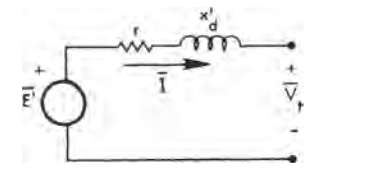
\includegraphics[height=0.1\textheight]{circuito_reattanza}
		\caption{Circuito transitorio equivalente }
	\end{figure}
	La tensione ai morsetti $\bar{V}$ è pari alla tensione interna del generatore (a vuoto) $\bar{E}$ meno la caduta di tensione sulla linea dovuta alla resistenza r e alla reattanza transitoria. Proprio perché la resistenza dei circuiti statorici è minima ciò che fondamentalmente lega la tensione a vuoto alla tensione ai morsetti è la reattanza transitoria in diretta $x'_d$.\\
	Il prossimo passo è quello di trovare le equazioni differenziali con le nostre nuove variabili. Iniziamo ad indagare dall' asse in diretta:\\
	\[
	\begin{cases}
	\Psi_d=L_dI_d+kM_fI_f\\
	\Psi_f=kM_fI_d+L_fI_f \rightarrow I_f=\frac{\Psi_f-kM_fI_d}{L_f}
	\end{cases}
	\]
	Eliminando $I_f$ dalla prima equazione utilizzando la seconda:\\
	$\Psi_d=L_dI_d+\frac{kM_f\Psi_f}{L_f}-\frac{(kM_f)^2}{L_f}I_d$.\\
	Riconosciamo qui la presenza di $L_d-\frac{(kM_f)^2}{L_f}=L'_d$, e una quantità che è proprio la tensione di picco, $\frac{kM_f\Psi_f}{L_f}$. Per capire meglio la natura dell' ultimo termine troviamo l' espressione della f.e.m. nel circuito fittizio sull' asse d quando la macchina è scollegata da un carico:\\
	$\Psi_f=L_fI_f \rightarrow I_f=\frac{\Psi_f}{L_f}$;\\
	$\Psi_d=kM_fI_f=kM_f\frac{\Psi_f}{L_f}$.\\Ora che conosciamo il flusso in diretta dovuto all' esistenza del circuito di field alimentato in continua possiamo dire che la f.e.m. in diretta si trova derivando ambo i membri:\\
	$\dot{\Psi}_d=kM_f\frac{\dot{\Psi}_f}{L_f}$, ed essendo tutte queste variabili funzioni sinusoidali con pulsazione $\omega_r$ allora questa f.e.m. avrà un picco di $kM_f\omega_r\frac{\Psi_f}{L_f}$, ma siccome $\omega_r\simeq1$, allora la quantità $kM_f\frac{\Psi_f}{L_f}$ è il picco della f.e.m. nel circuito d e definiremo $e'_q=kM_f\frac{\Psi_f}{L_f}$, quindi:\\
	$\Psi_d=L'_dI_d+e'_q$.\\\\
	Ragionando similmente per l' asse q prendiamo le equazioni di interesse\\
	\[
	\begin{cases}
	\Psi_q=L_qI_q+kM_QI_Q\\
	\Psi_Q=L_QI_Q+kM_QI_q \rightarrow I_Q=\frac{\Psi_Q-kM_QI_q}{L_Q}
	\end{cases}
	\]
	e sostituendo l' espressione di $I_Q$ nella prima equazione si ottiene:\\
	$\Psi_q=L_qI_q+\frac{kM_Q\Psi_Q}{L_Q}-\frac{(kM_Q)^2}{L_Q}I_q$,\\
	e riconoscendo il flusso transitorio in diretta ($\Psi_q-L'_qI_q$) e ricordando che $e'_d=-\omega_r\Psi'_q\simeq -\Psi'_q$,\\
	$e'_d=-\frac{kM_Q\Psi_Q}{L_Q}$.\\
	Utilizzando l' equazione della tensione sul circuito di rotore Q, $\dot{\Psi}_Q+r_QI_Q=0$, con una serie di manipolazioni e tenendo conto di tutte le quantità che sono state ricavate si ottiene:\\
	$\tau'_{d0} \dot{E'_d}=-E'_d-(x_q-x'_q)I_q$, \\dove
	\[
	\begin{cases}
	e'_d=\sqrt{3}E'_d\\
	e'_q=\sqrt{3}E'_q
	\end{cases}
	\]\\
	Svolgendo calcoli analoghi per l' equazione del circuito di field si ottiene:\\
	$\dot{E'_q}=\frac{1}{\tau'_{d0}}(E_{FD}-E)$,\\
	dove $E_{FD}=\omega_rkM_f(\frac{V_f}{r_f})$, è la f.e.m. di statore quando ci si trova in condizioni di steady-state, per questo $I_f=\frac{V_f}{r_f}$, visto che le le derivate a regime sono nulle; inoltre $\sqrt{3}E=e_q=kM_fI_f$, e vale anche la relazione:\\ $E+x_dI_d=E'_d+x'_dI_d$.\\
	Ora riprendendo l' equazione della coppia ed effettuando alcune manipolazioni si ha che\\
	$C_e=\frac{C_{e\phi}}{3}=\frac{L_dI_dI_q+kM_QI_dI_Q+kM_fI_qI_f-L_qI_dI_q}{3}=E'_dI_d+E'_qI_q-(L'_q-L'_d)I_qI_d$.\\
	Inserendola quindi nell' equazione della dinamica del rotore:\\
	$\tau_j\dot{\omega}=C_m-D\omega-E'_dI_d+E'_qI_q-(L'_q-L'_d)I_qI_d$.\\
	L' equazione della dinamica del load angle invece rimane inalterata, quindi possiamo formulare il modello con lo spazio di stato del IV ordine, poiché avremo due differenziali per i due assi del rotore, un' equazione differenziale per la dinamica del rotore e una per la dinamica del load angle. Le variabili di stato quindi saranno: $x=[E'_d,E'_q,\omega,\delta]$ e gli ingressi invece saranno $u=[I_d,I_q,C_m,E_{FD}]$. Si può notare quindi che avendo generato un modello in cui le variabili di stato sono delle tensioni, più precisamente delle tensioni a vuoto nel regime transitorio, e gli ingressi $V_d$ e $V_q$ di cui si era parlato in precedenza, dipendenti dalla struttura della rete, quindi del carico agganciato, sono stati sostituiti rispettivamente da $I_d$ e $I_q$.\\
	Il modello definitivo:\\
	\[
	\begin{cases}
	\tau'_{q0} \dot{E'_d}=-E'_d-(x_q-x'_q)I_q\\
	\tau'_{d0}\dot{E'_q}=E_{FD}-E'_q+(x_d-x'_d)I_d\\
	\tau_j\dot{\omega}=C_m-D\omega-E'_dI_d+E'_qI_q-(x'_q-x'_d)I_qI_d\\
	\dot{\delta}=\omega-1
	\end{cases}
	\]
	\chapter{}
	\section{Studio della rete WSCC-9}
	\subsection{Generalità}
	La Western System Coordinating Council (WSCC-9) è una rete elettrica che conta 9 bus, 3 macchine sincrone e 8 linee di trasmissione. Essa è una rete molto ampia, situata in America che si snoda in molti stati.
	\begin{figure}
		\centering
		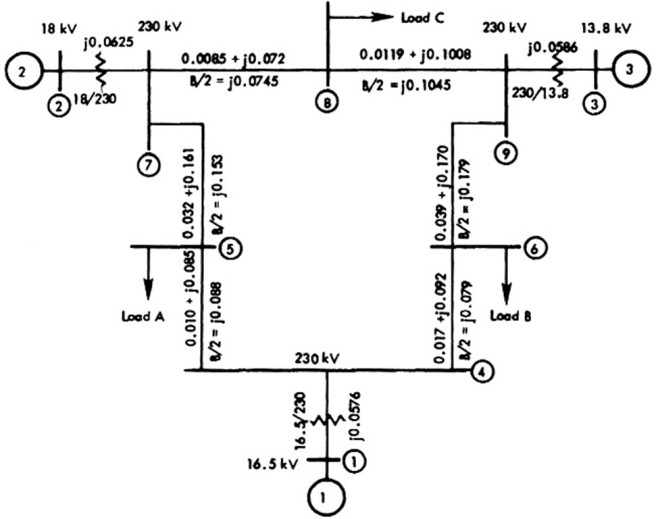
\includegraphics[height=0.35\textheight]{WSCC_line}
		\caption{Grafico della rete WSCC-9}
	\end{figure}
	Quello in figura 2.1 è un grafico della rete che si trova in letteratura, che data la grande numerosità degli elementi interconnessi in questione viene presentato già ridotto. I cerchi numerati rappresentano le macchine sincrone, che in realtà sono un agglomerato di macchine, che lavorano insieme e vengono sintetizzate come un singolo alternatore. I bus sono numerati da 1 a 9 e le linee invece, che collegano un bus ad un altro sono caratterizzate da un' impedenza. Una linea di trasmissione è un oggetto fisico che si estende per molti km, ed è proprio per questo che le equazioni differenziali che descrivono la propagazione dei segnali sono alle derivate parziali, poiché il tempo di trasmissione del segnale non è trascurabile. E' per questo che si usano dei modelli equivalenti della linea che ben sintetizzano il suo comportamento. Uno di questi è il modello pi-greco, dove compare un parametro caratteristico della linea, che è una suscettanza e nel grafico viene indicata con B/2; essa modella gli effetti di conduzione che si verificano tra i conduttori e i conduttori a terra, come se vi fosse un condensatore con una propria capacità. Un altro elemento fondamentale che si nota sul grafico è il trasformatore, ed essendo questa una rete di trasmissione, i trasformatori sono di tipo step-up, che alzano la tensione alla sbarra della macchina fino a quella adatta per la trasmissione, che in questo caso è di 230kV. La rete trasmette energia elettrica a tre carichi A,B,C (bus 5,6,8), che non sono veri e propri carichi, ma rappresentano la domanda di potenza, attiva e reattiva, che viene richiesta dai sottosistemi di distribuzione. Le caratteristiche delle tra macchine sono sintetizzate nella tabella in figura 2.2.
	\begin{figure}
		\centering
		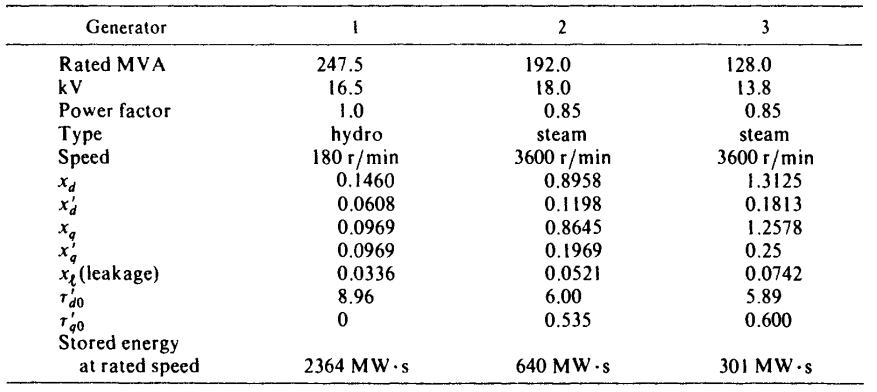
\includegraphics[height=0.25\textheight]{macchineWSCC}
		\caption{Dati delle tre macchine sincrone [1]}
	\end{figure}
	Un' informazione importante che può essere ricavata dalla tabella è proprio la differenza fondamentale tra la macchina 1 e le altre due. La prima è una macchina che lavora in una centrale idroelettrica, ciò vuol dire che è a poli salienti, mentre le altre due sono dei turbogeneratori, quindi lavorano in centrali termoelettriche. Questa differenza è testimoniata sia dai valori molto diversi della velocità angolare che raggiunge il rotore, sia dalle costanti $x_q$ e $x'_q$. Nel caso della macchina a poli salienti, in cui il blocco solido di metallo del rotore non offre un passaggio naturale per le correnti parassite, la differenza tra la reattanza in quadratura sincrona e quella transitoria non c'è, mentre è piuttosto elevata nelle altre due. Questo perché come già detto il blocco di metallo nel caso dei turbogeneratori si comporta come un circuito aggiuntivo naturale in quadratura, che entra in gioco nei transitori.
	\subsection{Modellazione matematica della rete}
	Nel capitolo 1 di questo lavoro si è ottenuto un modello della macchina sincrona, a dispetto del carico ad essa collegato, e quindi sappiamo quali sono le equazioni differenziali che governano le variabili di nostro interesse. E' doveroso però fare una precisazione circa il riferimento che bisogna scegliere. Sappiamo che a monte è già stata fatta una trasformazione nel dominio di Park, attraverso una matrice di trasformazione. Nel caso del multimacchina però ogni trasformata è stata fatta a sé, secondo il riferimento della macchina in questione, che si ricordi è dato dalla direzione del flusso del campo nella fase A. Ci sarà quindi bisogno di cambiare questo riferimento e renderlo uniforme per lo studio successivo, ma questo sarà fatto più avanti.\\
	Per ora ci limitiamo a fare delle considerazioni preliminari che portano alla determinazione della matrice delle ammettenze, che descrive matematicamente la struttura della rete. Quest' ultima per ora può essere vista come nella figura 2.3.
	\begin{figure}
		\centering
		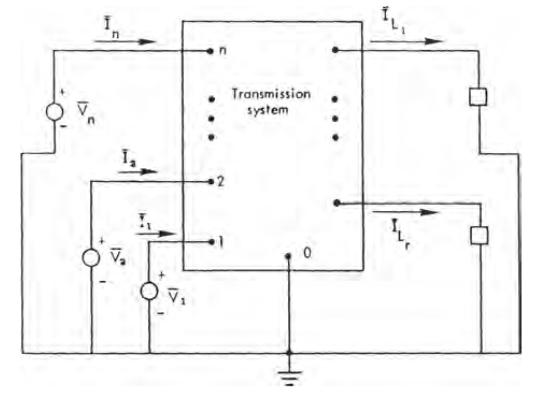
\includegraphics[height=0.3\textheight]{nonridotta}
		\caption{Schema semplificato non ridotto di una rete[1]}
	\end{figure}
	Vi sono n generatori di tensione, che stanno a modellare le tensioni ai morsetti di ogni macchina sincrona, vi è un blocco unico che rappresenta i vari collegamenti tra sorgenti e carichi, e vi sono infine r carichi che hanno una certa richiesta di potenza.
	Il prossimo passo è quello di trasformare ogni bus di carico in un' ammettenza shunt equivalente. I bus di carico sono appunto dei bus che hanno una certa richiesta di potenza attiva e reattiva, che non sono funzioni del tempo. Infatti immagineremo di porci nel caso in cui le richieste di potenza da parte dei carichi siano fisse, e lavoreremo in quell' intorno, e proprio per questo è possibile eliminare ogni bus di carico trasformando lo stesso in un' ammettenza shunt (come se fosse una dispersione di corrente a terra) equivalente. Il procedimento preliminare da seguire è descritto qui in breve.\\
	Immaginiamo che l' i-esimo bus abbia tensione $\bar{V}_L$, potenza attiva $P_L$, potenza reattiva $Q_L$, e che nel bus fluisca una corrente $\bar{I}_L$, allora:\\
	$P_L+jQ_L=\bar{V}_L\bar{I}^*_L=\bar{V}_L[\bar{V}^*_L(G_L-jB_L)]=V_L^2(G_L-jB_L)$, quindi l' ammettenza shunt (quindi considerata come una dispersione di corrente a terra) equivalente è\\
	$\bar{Y}_L=P_L/V^2_L-j(Q_L/V^2_L)$.\\
	Prima di determinare la matrice delle ammettenze c'è da fare una precisazione. Come è possibile notare nella figura 2.1 i bus a cui sono collegati i generatori sono le "sbarre" a cui arrivano i morsetti dei circuiti statorici, cioè dove si misura la tensione $\bar{V}$, e le relazioni tra tensioni e correnti tengono appunto in considerazione queste tensioni, che però cozzano con la nostra scelta delle variabili di stato per la modellazione della macchina sincrona, che usano le tensioni a vuoto dei generatori. Come è già stato fatto notare nella sezione 1.3 però, il parametro che lega le tensioni a vuoto con le tensioni alla sbarra è la reattanza transitoria $x'_d$. Proprio per riportare le relazioni tra $\bar{V}$ e $\bar{I}$ in relazioni tra $\bar{E}$ e $\bar{I}$ verrà inglobata la reattanza transitoria nella matrice delle ammettenze. In particolare $x'_d$ verrà sommata alla ammettenza del trasformatore che segue sempre la macchina.
	Una volta effettuato ciò è possibile determinare la matrice delle ammettenze $\bar{Y}$ seguendo delle regole:\\\\
	1. Ogni impedenza deve essere trasformata in un' ammettenza equivalente;\\
	2. Ogni ammettenza shunt di carico deve essere considerata collegata al bus;\\
	3. $\bar{Y}_{ii}$ è pari alla somma delle ammettenze connesse al nodo i-esimo, mentre $\bar{Y}_{ij}$ è pari all' ammettenza tra i nodi i e j cambiata di segno.\\
	Il passo successivo è quello di operare la riduzione di Kronn, che è basata sul concetto secondo il quale ogni macchina sincrona può essere vista come una f.e.m. che è equivalente a un generatore di corrente con in parallelo un impedenza. La chiave fondamentale è che ogni macchina può essere vista come un generatore di corrente che inietta corrente nella rete, mentre ogni carico è solo un' impedenza costante che costituisce una certa richiesta di potenza, e quindi non immette nulla in rete. Essendo la corrente iniettata dai carichi nulla si può effettuare la seguente partizione:\\
	$\begin{bmatrix}
	\bar{I}_n\\
	0
	\end{bmatrix}=
	\begin{bmatrix}
	Y_{nn} & Y_{nr}\\
	Y_{rn} & Y_{rr}
	\end{bmatrix}
	\begin{bmatrix}
	\bar{V}_n\\
	\bar{V}_r
	\end{bmatrix}$\\
	dove il pedice n indica le grandezze che si riferiscono alle macchine e r quelle che si riferiscono ai carichi.\\
	Dalla seconda equazione possiamo ricavare $\bar{V}_r=-Y^{-1}_{rr}Y_{rn}\bar{V}_n$, e sostituire nella prima trovando che\\
	$\bar{I}_n=Y_{nn}\bar{V}_n-Y_{nr}Y^-1_{rr}Y_{rn}\bar{V}_n=(Y_{nn}-Y_{nr}Y^{-1}_{rr}Y_{rn})\bar{V}_n=Y_{\text{rid}}\bar{V}_n$. Omettendo i calcoli si ha in questo caso:\\\\
	$Y_{rid}=
	\begin{bmatrix}
	0.8455-j29883 & 0.2871+j1.5129 & 0.2096+j1.2256\\
	0.2871+j1.5129 & 0.4200-j2.7238 & 0.2133+1.0879\\
	0.2096+j1.2256 & 0.2133+j1.0879 & 0.2770-j2.3681
	\end{bmatrix}$\\\\
	Così facendo è stato possibile trovare una matrice delle ammettenze ridotte di dimensione nxn, se n è il numero delle macchine nella rete. Questa riduzione è solo possibile sotto le ipotesi fatte in precedenza.
	Dopo queste considerazioni preliminari possiamo vedere la rete sintetizzata in figura 2.4.
	\begin{figure}
		\centering
		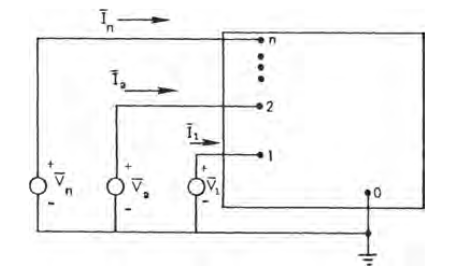
\includegraphics[height=0.25\textheight]{ridotta}
		\caption{Schema semplificato e ridotto secondo Kronn[1]}
	\end{figure}
	Avendo quindi definito i vettori\\\\\\ di tensioni e correnti delle macchine:\\
	$\bar{V}=\begin{bmatrix}
	V_{q1}+jV_{d1}=\bar{V}_1\\
	V_{q2}+jV_{d2}=\bar{V}_2\\
	...\\
	V_{qn}+jV_{dn}=\bar{V}_n
	\end{bmatrix}$\qquad
	$\bar{I}=\begin{bmatrix}
	I_{q1}+jI_{d1}=\bar{I}_1\\
	I_{q2}+jI_{d2}=\bar{I}_2\\
	...\\
	I_{qn}+jI_{dn}=\bar{I}_n
	\end{bmatrix}$\\
	c'è da considerare il fatto che la trasformazione di Park, come già accennato, è stata effettuata in maniera a sé stante per ciascuna macchina, senza considerare un riferimento comune.
	Prendiamo in considerazione un ramo i-esimo della rete nel transitorio:\\
	esso è caratterizzato da una resistenza $r_i$, da un' induttanza $l_i$ e quindi da un' impedenza $\bar{z}_i$. Allora vale la relazione:\\
	$v_{abci}=r_ii_{abci}+l_i\dot{i}_{abci}$, con $i=1...b$, dove b è il numero di rami.
	Possiamo quindi operare la trasformazione di Park:\\
	$Pv_{abci}=r_iPi_{abci}+l_iP\dot{i}_{abci}$, e sfruttando le relazioni nel primo capitolo, sempre in caso di carico bilanciato,\\ $v_{dqi}=r_ii_{dqi}+l_i(\dot{i}_{dqi}-\omega\begin{bmatrix}
	-i_{qi}\\
	i_{di}
	\end{bmatrix})$.\\
	Considerando $\omega \simeq 1$ possiamo dire che la quantità $\omega l_i \simeq x_i$, e considerando anche trascurabili i termini $l_i\dot{i}_i$ se confrontati con $\omega l_ii_i$ allora:\\
	$v_{dqi}=r_ii_{dqi}+x_i(\begin{bmatrix}
	i_{qi}\\
	-i_{di}
	\end{bmatrix})$.\\ 
	Moltiplicando ambo i membri per $\frac{1}{\sqrt{3}}$ e sfruttando le relazioni:\\
	\[
	\begin{cases}
	v_q=\sqrt{3}V_q\\
	v_d=\sqrt{3}V_d\\
	i_q=\sqrt{3}I_q\\
	i_d=\sqrt{3}I_d\\
	\end{cases}
	\]
	allora $V_{dqi}=r_iI_{dqi}+x_i(\begin{bmatrix}
	I_{qi}\\
	-I_{di}
	\end{bmatrix})$\\\\\\
	Abbiamo quindi che:\\
	$V_{qk(i)}=r_kI_{qk(i)}-x_kI_{dk(i)}$,\\
	$V_{dk(i)}=r_kI_{dk(i)}+x_kI_{qk(i)}$.\\
	Di conseguenza possiamo accorpare le equazioni \\
	$\bar{V}_{k(i)}=V_{qk(i)}+jV_{dk(i)}=r_kI_{qk(i)}-x_kI_{dk(i)}+j(r_kI_{dk(i)}+x_kI_{qk(i)})=\\
	(r_k+jx_k)(I_{qk(i)}+jI_{dk(i)})=\bar{z}_k\bar{I}_{k(i)}$.\\
	Il pedice (i) sta a significare che le trasformazioni di Park sono state effettuate rispetto al riferimento della macchina i-esima. Questo è il passo preliminare che ci permette poi di rendere comuni tutti i riferimenti. Abbiamo per questo bisogno di un riferimento sincrono rotante alla velocità di regime, che verrà eletto come riferimento comune per tutte. Se assumiamo che in condizioni di equilibrio la rete ha una propria velocità di sincronismo e le velocità angolari dei rotori coincidono, capiamo bene che ciò che distingue il riferimento di una macchina da quello sincrono è un angolo di sfasamento che viene misurato tra l' asse q della macchina i-esima e l' asse q della macchina di riferimento. Per avere più chiaro il concetto è possibile riferirsi alla figura 2.5.
	\begin{figure}
		\centering
		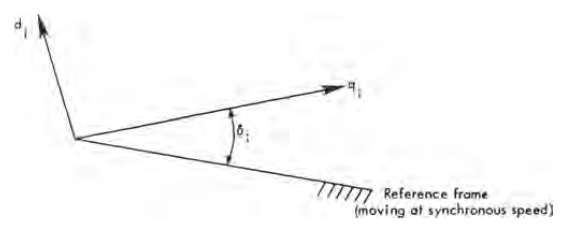
\includegraphics[height=0.2\textheight]{riferimento_comune}
		\caption{Angolo di sfasamento tra la macchina i-esima e il riferimento}
	\end{figure}\\
	Proprio per questo motivo per passare da un riferimento a un altro basta effettuare una rotazione secondo l' angolo che si individua tra i due assi.
	\\
	La matrice di rotazione in due dimensioni (date dall' asse d e q), è:\\
	$R=\begin{bmatrix}
	\cos(\alpha) & -\sin(\alpha)\\
	\sin(\alpha) & \cos(\alpha)
	\end{bmatrix}$. \\
	Vogliamo convertire il vettore $\bar{V}_{i}=V_{qi}+jV_{di}$ in un vettore $\bar{V}_{i}=V_{Qi}+jV_{Di}$.\\
	$\begin{bmatrix}
	V_Q\\
	V_D
	\end{bmatrix}=
	\begin{bmatrix}
	\cos(\delta_i) & -\sin(\delta_i)\\
	\sin(\delta_i) & \cos(\delta_i)
	\end{bmatrix}
	\begin{bmatrix}
	V_q\\
	V_d
	\end{bmatrix}$, quindi:\\
	$V_{Qi}+jV_{Di}=V_{qi}\cos(\delta_i)-V_{di}\sin(\delta_i) +j(V_{qi}\sin(\delta_i)+V_{di}\cos(\delta_i))$.\\
	Possiamo sintetizzare l' espressione scrivendola come\\
	$\hat{V}_i=\bar{V}_ie^{j\delta_i}$, dove $\hat{V}$ è il vettore di tensione riferito al nuovo sistema di assi. Di conseguenza abbiamo che:\\
	$\bar{V}_i=\hat{V}_ie^{-j\delta_i}$, quindi la trasformazione avverrà semplicemente attraverso una rotazione, il che risulta intuitivo se si guarda la figura 2.6.
	\begin{figure}
		\centering
		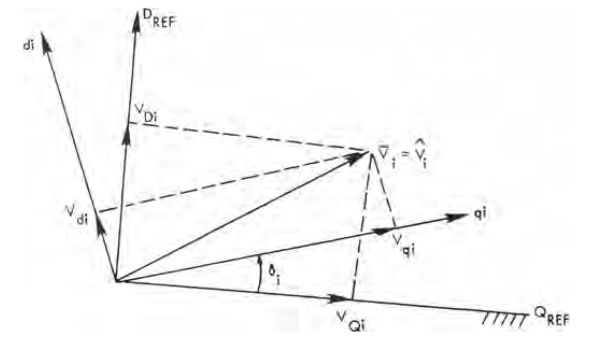
\includegraphics[height=0.3\textheight]{cambio_coordinate}
		\caption{Riferimento $V_{QD}$ e $V_{qd}$}
	\end{figure}
	Per effettuare il cambio di riferimento prendiamo l' equazione della caduta di tensione in un ramo:\\
	$\bar{V}_k=\bar{z}_kI_k \quad \rightarrow \quad \hat{V}_ke^{-j\delta_k}=\bar{z}_k\hat{I}_ke^{-j\delta_k} \quad \rightarrow \quad \hat{V}_k=\bar{z}_k\hat{I}_k$, o equivalentemente,\\$\hat{I}_k=\bar{y}_k\hat{V}_k$.\\
	Avendo già trovato la matrice delle ammettenze ridotte è possibile trasformare la relazione precedente in una relazione vettoriale che tiene conto di tutti i nodi,
	\begin{equation}
		\hat{I}=\bar{Y}\hat{V}
	\end{equation}
	Di conseguenza anche la trasformazione del riferimento può essere generalizzata per tutti i nodi usando una matrice di trasformazione\\
	$T=\begin{bmatrix}
	e^{j\delta_1} & 0 & ... & 0\\
	0 & e^{j\delta_2} & ... & 0\\
	... & ...  & ... & ...\\
	0 & 0 & ... & e^{j\delta_n}
	\end{bmatrix}$\\
	Se T è la matrice che permette la rotazione in un verso, quella nel senso opposto viene ottenuta utilizzando $T^*$. Con pochi semplici passaggi, a partire dall' equazione 2.1 si ottiene:\\
	\begin{equation}
	\bar{I}=(T^{-1}\bar{Y}T)\bar{V}=\bar{M}\bar{V}
	\end{equation}
	Quest' ultima equazione è importante perché è quella che modella matematicamente la struttura della rete (interconnessione ridotta dei nodi) rispetto a un riferimento comune sincrono.\newpage
	\section{Linearizzazione}
	Dopo una breve introduzione al problema del Load Flow si procederà con la linearizzazione intorno al punto d' equilibrio sia della macchina sincrona sia della rete.
	\subsection{Determinazione del punto di lavoro}
	Il primo passo necessario per effettuare una linearizzazione di un sistema è scegliere il punto di lavoro adatto. Il punto di lavoro spesso è un equilibrio stabile del sistema, e lo si sceglie proprio perché a una perturbazione delle variabili dal punto di equilibrio segue un' evoluzione delle stesse che tende a diventare nulla al variare del tempo. Ma nel caso di un power system cosa si intende con punto di lavoro?\\
	Il punto di lavoro è il punto di inizio della nostra analisi, che ci da informazioni sui valori iniziali delle nostre variabili di stato. Un power system è composto sicuramente da generatori (nodi P-V) che producono energia, e da carichi (nodi P-Q), che sono bus con una certa domanda di potenza attiva e reattiva. Tra i generatori ne viene eletto uno (lo slack) che funge da riferimento rotante per tutti gli altri.\\ L' obiettivo di un power system, d' altronde, è quello di assicurare l' apporto di potenza ai carichi della rete, ed è proprio questo il motivo per cui ci si avvale del load flow per determinare il punto di lavoro. Il load flow è lo studio dei flussi di potenza nella rete a regime, al fine di soddisfare la richiesta da parte dei carichi, quindi viene condotto sulla rete non ridotta. Le incognite che compaiono sono $V_i,\delta_i,P_i,Q_i$, con $i=1,..,n$, dove $n$ è il numero di nodi, per un totale di $4n$ incognite.
	\begin{figure}
		\centering
		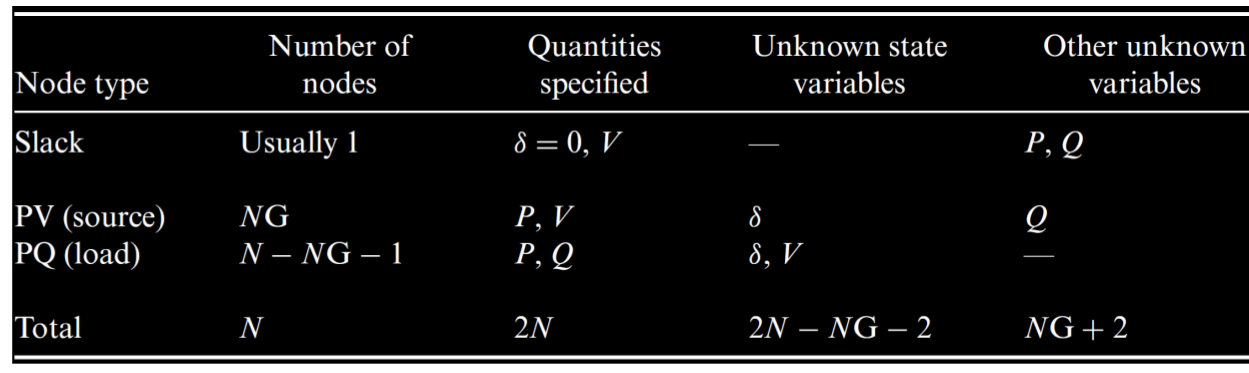
\includegraphics[height=0.15\textheight]{tipidibus}
		\caption{Tipi di bus, variabili conosciute e sconosciute}
	\end{figure} Determinando però la natura dei nodi è possibile ricavare $2n$ di queste (fig. 2.7), mentre le restanti, sempre $2n$, devono essere ricavate dalla rete. Le equazioni in questione possono essere ricavate in questo modo:\\
	$P+jQ=\bar{V}\bar{I}^* \rightarrow P+jQ=\bar{V}(\bar{Y}\bar{V})$, e separando parte immaginaria e parte reale si ottengono le $2n$ equazioni non lineari rimanenti del tipo:\\
	\[
	\begin{cases}
	P=f(V,\delta)\\
	Q=g(V,\delta)
	\end{cases}
	\]
	Questa tecnica si basa sul fatto che il load flow è uno studio che viene fatto all' equilibrio, in particolare $\dot{\omega}=0$, ed essendo le derivate nulle, è possibile fare un' analisi "statica" dei flussi di potenza. Sono delle equazioni non lineari, che per essere risolte necessitano di strumenti di risoluzione approssimati come Newton-Rhapson, Gauss-Seidel, Fast decouple. Esistono vari software per effettuare questa operazione, e il risultato del load flow effettuato sulla WSCC-9 è riportato in figura 2.8. Come si può vedere lo slack che funge da riferimento ha sfasamento angolare nullo, poiché come si è detto è il nostro riferimento. In figura è possibile vedere il modulo della tensione su ogni bus, la fase della tensione, la potenza attiva e la potenza reattiva, e quindi attraverso il load flow abbiamo ricavato tutte le informazioni necessarie.\\\\\\\\
	\begin{figure}[h]
		\centering
		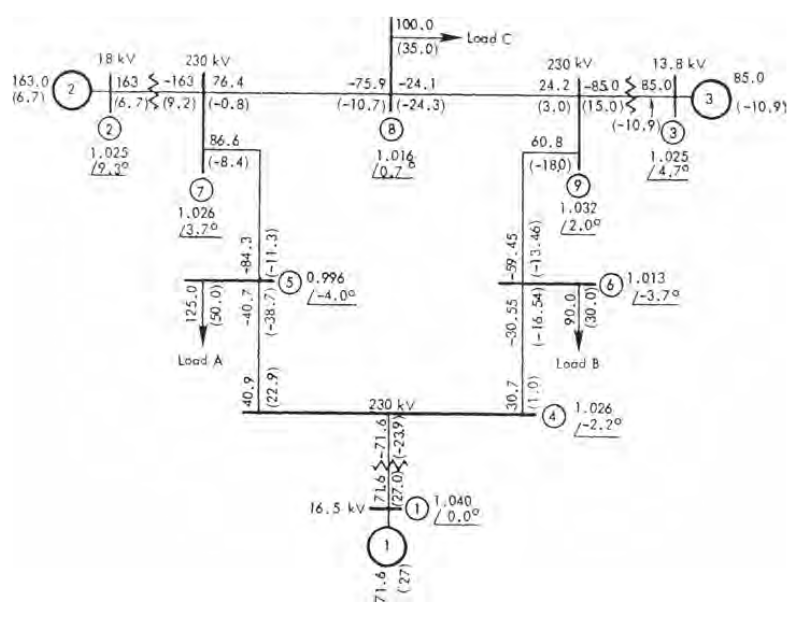
\includegraphics[scale=0.36]{WSCC-powerflow}
		\caption{Load flow WSCC-9 bus system}
	\end{figure}
	\subsection{Linearizzazione della macchina sincrona}
	Per quanto riguarda le macchine 2 e 3 ricorreremo allo spazio di stato ricavato nella sezione 1.3. Solitamente si fa l' approssimazione $x'_q\simeq x'_d$, cosicché la dinamica della coppia non dipenda più dal prodotto delle correnti, e si ottiene quindi:
	\[
	\begin{cases}
	\tau'_{q0} \dot{E'_d}=-E'_d-(x_q-x'_q)I_q\\
	\tau'_{d0}\dot{E'_q}=E_{FD}-E'_q+(x_d-x'_d)I_d\\
	\tau_j\dot{\omega}=C_m-D\omega-E'_dE'_q\\
	\dot{\delta}=\omega-1
	\end{cases}
	\]
	dove variabili di stato sono $x=[E_d,E_q,\omega,\delta]$.\\
	Il punto di lavoro definito attraverso il load flow è $x_0=[E_{d0},E_{q0},\omega_0,\delta_0]$, e quindi la linearizzazione viene fatta sostituendo al vettore perturbato \\$x'=x_0+x_\Delta$. All' equilibrio nel punto di lavoro le derivate sono nulle e si ricavano quindi le seguenti relazioni:\\
	\[
	\begin{cases}
	E'_{d0}=-(x_q-x'_q)I_{q0}\\
	E_{FD0}=E'_{q0}+(x'_d-x_d)I_{d0}\\
	C_{m0}=D\omega_0+E'_{d0}I_{d0}-E'_{q0}I_{q0}\\
	\omega_0=1
	\end{cases}
	\]
	Tenendo conto delle relazioni qui sopra ed eliminando i termini di grado superiore al primo si ottiene:
	\[
	\begin{cases}
	\tau'_{q0}\dot{E}'_d= -E'_d-(x_q-x'_q)I_q\\
	\tau'_{d0}\dot{E}'_q=E_{FD}-E'_q+(x_d-x'_d)I_d\\
	\tau_j\dot{\omega}=C_m-D\omega-I_{d0}E'_d-I_{q0}E'_q-E'_{d0}I_d-E'_{q0}I_q\\
	\dot{\delta}=\omega
	\end{cases}
	\]
	In questo lavoro siamo interessati a rappresentare in maniera dettagliata il comportamento delle variabili delle macchine 2 e 3, cioè dei turbogeneratori, mentre per la macchina 1, lo slack, si utilizzerà un modello meno preciso, che, sotto le ipotesi che seguono, tiene solo conto della dinamica del rotore:\\
	1. La potenza meccanica, e quindi la coppia, rimane costante durante il transitorio;\\
	2. La macchina può essere rappresentata da una tensione costante dietro reattanza transitoria.\\
	Data la vastità della rete,  è possibile rappresentare le zone di meno interesse con minor precisione.\\
	Prendendo in considerazione il modello a due assi si assume che:\\
	1. Il circuito sul rotore in quadratura è trascurabile, di conseguenza verrà eliminata l' equazione differenziale in diretta;\\
	2. $E'_q$ in modulo è uguale a $E'$, e differiscono tra loro di un angolo molto piccolo, di conseguenza $E'\simeq E'_q$;\\
	3. $E'_q$ rimane pressocché invariato durante il transitorio, quindi viene eliminata anche l' equazione differenziale in quadratura.\\
	Fatte queste assunzioni il modello linearizzato che verrà impiegato per la modellazione della macchina 1 è:\\
	\[
	\begin{cases}
	\tau_j\dot{\omega}=C_m-D\omega-E_0I_q\\
	\dot{\delta}=\omega
	\end{cases}
	\]
	dove $E_0=E'-(x_d-x'_d)I_{d0}$.
	\subsection{Linearizzazione della rete}
	L' operazione di linearizzazione ovviamente va fatta anche sulla rete, che è descritta dall' equazione 2.2, e quest' ultima può essere riscritta come:\\
	\begin{equation}
	\bar{I}_\Delta=\bar{M}_0\bar{V}_\Delta+\bar{M}_\Delta\bar{V}_0
	\end{equation}
	Per $\bar{M}_0$ si intende la matrice calcolata agli angoli iniziali $\delta_{i0}$ che vengono ricavati dal load flow.\\\\ Definendo $\delta_i=\delta_{i0}+\delta_{i\Delta}$ possiamo ricavare l' espressione estesa di M:\\
	$M=\begin{bmatrix}
	Y_{11}e^{j\theta_{11}} & Y_{12}e^{j(\theta_{12}-\delta_{120}-\delta_{12\Delta})} & ... & Y_{1n}e^{j(\theta_{1n}-\delta_{1n0}-\delta_{1n\Delta})}\\
	... & ... & ... & ...\\
	Y_{n1}e^{j(\theta_{n1}-\delta_{n10}-\delta_{n1\Delta})} & Y_{n2}e^{j(\theta_{n2}-\delta_{n20}-\delta_{n2\Delta})} & ... & Y_{nn}e^{j\theta_{nn}}
	\end{bmatrix}$\\
	Quindi gli elementi fuori dalla diagonale sono del tipo $m_{ij}=Y_{ij}e^{j(\theta_{ij}-\delta_{ij0}-\delta_{ij\Delta})}$, e approssimando $\cos(\delta_{ij\Delta})\simeq 1$, e $\sin(\delta_{ij\Delta})\simeq \delta_{ij\Delta}$, possiamo riscrivere:\\
	$m_{ij}=Y_{ij}e^{j(\theta_{ij}-\delta{ij0})}e^{-j\delta_{ij\Delta}}=Y_{ij}e^{j(\theta_{ij}-\delta{ij0})}(1-j\delta_{ij\Delta})$. Questa scrittura ci permette di separare agilmente i termini $m_{ij\Delta}$ dai termini $m_{ij0}$, quindi di separare rispettivamente $M_\Delta$ da $M_0$. Il generico termine $m_{ij\Delta}$ è pari a:\\ $m_{ij\Delta}=-jY_{ij}e^{j(\theta_{ij}-\delta{ij0})}\delta_{ij\Delta}$. Avendo separato in due parti distinte la matrice M è possibile scrivere in maniera estesa l' equazione 2.3 e dopo vari passaggi si arriva a una scrittura del tipo:\\
	\begin{equation}
	\resizebox{0.98\hsize}{!}{%
	$\begin{bmatrix}
	\bar{I}_{1\Delta}\\
	\bar{I}_{2\Delta}\\
	...\\
	\bar{I}_{n\Delta}\\
	\end{bmatrix}=
	\begin{bmatrix}
	Y_{11}e^{j\theta_{11}} & ... & Y_{1n}e^{j(\theta_{1n}-\delta_{1n0})}\\
	Y_{21}e^{j\theta_{21}} & ... & Y_{2n}e^{j(\theta_{2n}-\delta_{2n0})}\\
	... & ... & ...\\
	Y_{n1}e^{j(\theta_{n1}-\delta_{n10})} & ... & Y_{nn}e^{j\theta_{nn}}
	\end{bmatrix}
	\begin{bmatrix}
	\bar{V}_{1\Delta}\\
	\bar{V}_{2\Delta}\\
	...\\
	\bar{V}_{n\Delta}\\
	\end{bmatrix}-j
	\begin{bmatrix}
	\sum_{k=1}^{n}\bar{V}_{k0}Y_{1k}e^{j(\theta_{1k}-\delta{1k0})}\delta_{1k\Delta}\\
	\sum_{k=1}^{n}\bar{V}_{k0}Y_{2k}e^{j(\theta_{2k}-\delta{2k0})}\delta_{2k\Delta}\\
	...\\
	\sum_{k=1}^{n}\bar{V}_{k0}Y_{nk}e^{j(\theta_{nk}-\delta{nk0})}\delta_{nk\Delta}\\
	\end{bmatrix}$
	}
	\end{equation}
	Riportandoci nel nostro caso (3 macchine), e ricordando che avendo annesso la reattanza transitoria della macchina come un' effettiva reattanza della linea, le tensioni alla sbarra $\bar{V}_i$ possono essere sostituite con le tensioni a vuoto $\bar{E}_i$, l' equazione 2.4 diventa:\\
	\begin{equation}
	\resizebox{\hsize}{!}{$%
		\begin{bmatrix}
		\bar{I}_{1\Delta}\\
		\bar{I}_{2\Delta}\\
		\bar{I}_{3\Delta}\\
		\end{bmatrix}=
		\begin{bmatrix}
		Y_{11}e^{j\theta_{11}} & Y_{12}e^{j(\theta_{12}-\delta_{120})} & Y_{13}e^{j(\theta_{13}-\delta_{130})} & -j\bar{E}_{20}Y_{12}e^{j(\theta_{12}-\delta_{120})} & -j\bar{E}_{30}Y_{13}e^{j(\theta_{13}-\delta_{130})} & 0\\
		Y_{21}e^{j(\theta_{21}-\delta_{210})} & Y_{22}e^{j\theta_{22}} & Y_{23}e^{j(\theta_{23}-\delta_{230})} & -j\bar{E}_{10}Y_{21}e^{j(\theta_{21}-\delta_{210})} & 0 & -j\bar{E}_{30}Y_{23}e^{j(\theta_{23}-\delta_{230})}\\
		Y_{31}e^{j(\theta_{31}-\delta_{310})} & Y_{22}e^{j(\theta_{32}-\delta_{320})} & Y_{33}e^{j\theta_{33}} & 0 & -j\bar{E}_{10}Y_{31}e^{j(\theta_{31}-\delta_{310})} & -j\bar{E}_{20}Y_{32}e^{j(\theta_{32}-\delta_{320})}\\
		\end{bmatrix}
		\begin{bmatrix}
		\bar{E'}_{1\Delta}\\
		\bar{E'}_{2\Delta}\\
		\bar{E'}_{3\Delta}\\
		\delta_{12}\\
		\delta_{13}\\
		\delta_{23}
		\end{bmatrix}
		$%
	}%
	\end{equation}
	\begin{figure}
		\centering
		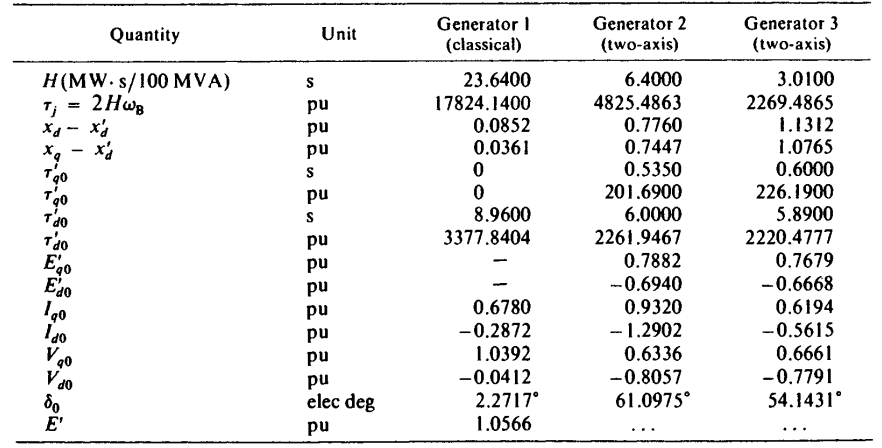
\includegraphics[height=0.28\textheight]{valori_loaflow1}
		\caption{Parametri e valori iniziali delle tensioni e delle correnti}
	\end{figure}
	\begin{figure}
		\centering
		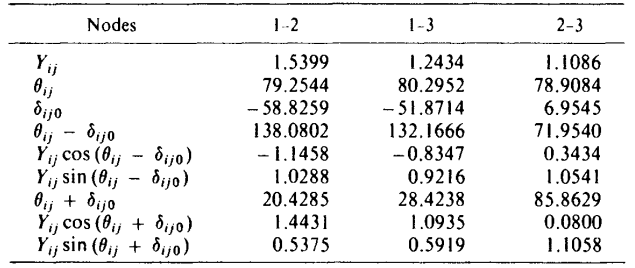
\includegraphics[height=0.2\textheight]{valori_loadflow2}
		\caption{Valori degli angoli noti}
	\end{figure}
	L' equazione 2.5 non è definitiva poiché mancano ancora delle considerazioni da fare. Avendo scelto la macchina 1 come slack, che è rappresentata in maniera classica, si avrà che la tensione $E'_{10}=E'_1$ e $E'_{1\Delta}=0$. Inoltre lo sfasamento angolare deve essere calcolato rispetto al riferimento, cioè la macchina 1, quindi non ha senso parlare di $\delta_{23}$, che deve essere sostituito da $\delta_{23}=\delta_{12}-\delta_{13}$. Utilizzando i valori ricavati dopo lo studio del load flow, che vengono riportati in figura 2.9 e 2.10, e tenendo conto delle considerazioni precedentemente fatte, dividendo parte reale e immaginaria si ottiene:\\
	\begin{equation}
	\begin{bmatrix}
	I_{q1\Delta}\\
	I_{d1\Delta}\\
	I_{q2\Delta}\\
	I_{d2\Delta}\\
	I_{q3\Delta}\\
	I_{d3\Delta}\\
	\end{bmatrix}=
	\begin{bmatrix}
	-1.1458 & -1.0288 & -0.8347 & -0.9216 & 1.6062 & 1.2642\\
	1.0288 & -1.1458 & 0.9216 & -0.8347 & 0.1891 & 0.0265\\
	0.4200 & 2.7239 & 0.3434 & -1.0541 & -1.1484 & 0.5805\\
	-2.7239 & 0.4200 & 1.0541 & 0.3434 & 2.4914 & -0.9666\\
	0.0800 & -1.1058 & 0.2770 & 2.3681 & 0.8160 & -1.4414\\
	1.1058 & 0.0800 & -2.3681 & 0.2770 & -0.8305 & 1.9859
	\end{bmatrix}
	\begin{bmatrix}
	E'_{q2\Delta}\\
	E'_{d2\Delta}\\
	E'_{q3\Delta}\\
	E'_{d3\Delta}\\
	\delta_{12\Delta}\\
	\delta_{13\Delta}\\
	\end{bmatrix}
	\end{equation}
	\\
	Prendendo il modello con lo spazi di stato linearizzato dei tre generatori si possono usare le relazioni 2.6 per eliminare le correnti dal modello e rendere le tensioni interne dei nodi le uniche variabili di stato. Avremo quindi uno spazio di stato generale che tiene conto del sistema complessivo interconnesso. Il vettore di stato terrà conto di tutte le variabili delle tre macchine (generatore 1 rappresentato classicamente e generatori 2 e 3 rappresentati con il modello due assi), e sarà pertanto:\\
	$x=[\omega_1 \quad E'_{q2} \quad E'_{d2} \quad \omega_2 \quad E'_{q3} \quad E'_{d3} \quad \omega_3 \quad \delta_{12} \quad \delta_{13}]$.\\
	Gli ingressi del sistema invece saranno:\\
	$u=[C_{m1} \quad E_{fd2} \quad C_{m2} \quad E_{fd3} \quad C_{m3}]$.\\\\\\\\\\\\\\
	Omettendo il pedice $\Delta$ si ottiene quindi:
	\begin{equation*}
	\centering
	\resizebox{1.04\hsize}{!}{$%
	\begin{bmatrix}
	\dot{\omega}_1\\
	\dot{E'}_{q2}\\
	\dot{E'}_{d2}\\
	\dot{\omega}_2\\
	\dot{E'}_{q3}\\
	\dot{E'}_{d3}\\
	\dot{\omega}_3\\
	\dot{\delta}_{12}\\
	\dot{\delta}_{13}
	\end{bmatrix}=10^{-4}
	\begin{bmatrix}
	-0.5610 & 0.6793 & 0.6099 & 0 & 0.4948 & 0.5463 & 0 & -0.9520 & -0.7494\\
	0 & -13.7658 & 1.4409 & 0 & 3.6163 & 1.1781 & 0 & 8.5472 & -3.3161\\
	0 & -15.5076 & -150.1554 & 0 & -12.6793 & 38.9205 & 0 & 42.4023 & -21.4333\\
	0 & -6.5352 & -1.1714 & -2.0723 & 0.9552 & 2.2156 & 0 & 5.4592 & -2.3385\\
	0 & 5.6334 & 0.4076 & 0 & -16.5675 & 1.4111 & 0 & -4.2309 & 10.1170\\
	0 & -3.8073 & 52.6270 & 0 & -13.1829 & -156.9117 & 0 & -38.8349 & 68.5987\\
	0 & 2.9781 & 3.9766 & 0 & -10.6238 & -4.7247 & -4.4063 & -5.2010 & 10.7116\\
	10000 & 0 & 0 & -10000 & 0 & 0 & 0 & 0 & 0\\
	10000 & 0 & 0 & 0 & 0 & 0 & -10000 & 0 & 0
	\end{bmatrix}
	\begin{bmatrix}
	\omega_1\\
	E'_{q2}\\
	E'_{d2}\\
	\omega_2\\
	E'_{q3}\\
	E'_{d3}\\
	\omega_3\\
	\delta_{12}\\
	\delta_{13}
	\end{bmatrix}+$%
	}%
	\end{equation*}
	\begin{align*}
	\resizebox{0.2\hsize}{!}{$%
	+10^{-4}\begin{bmatrix}
	0.5610C_{m1}\\
	4.4210E_{FD2}\\
	0\\
	2.0723C_{m2}\\
	4.5035E_{FD3}\\
	0\\
	4.4063C_{m3}\\
	0\\
	0
	\end{bmatrix}$%
	}%
	\end{align*}
	\chapter{}
	\section{Approccio controllistico alla WSCC-9}
	\subsection{Generalità}
	Il controllo di un power system può essere fatto a vari livelli, a seconda delle variabili che si vogliono controllare ed a seconda di dove avviene il controllo.\\
	Per quanto riguarda la sede delle unità di controllo si possono distinguere tre diversi gruppi:\\
	1. Controllo a monte delle unità di generazione;\\
	2. Controllo delle unità di generazione;\\
	3. Controllo del sistema di trasmissione (a valle delle unità di generazione).\\
	Il primo è un controllo ad alto livello e sostanzialmente si occupa di stabilire il set point di generazione di potenza, cercando di bilanciare la domanda della rete. E' un controllo che viene fatto a monte delle centrali e tiene conto anche dei risvolti economici. Il secondo gruppo riguarda i controlli che vengono svolti nelle centrali di generazione di energia elettrica, e vi rientrano vari tipi di controllo a seconda della variabile che si prende in considerazione. In linea generale si può dire che di questo gruppo fa parte il controllo di frequenza effettuato dal prime mover governor e dallo speed governor, che insieme costituiscono un apparato che gestisce la generazione di potenza primaria e la quantità di potenza che raggiunge effettivamente la turbina, in funzione della frequenza del rotore della macchina, che viene accelerato o decelerato dalla coppia elettrica che proviene dalla rete (controllo primario di frequenza);
	a fianco di questo controllo troviamo il sistema di eccitazione, che si occupa di generare la tensione di field. Qui hanno sede controllori come l' Automatic Voltage Regulator (AVR), che modifica la tensione di field in ingresso alla macchina per bilanciare i cali o gli aumenti di tensione registrati sullo statore, e il Power System Stabilizer, che funge da supporto all' AVR, in un modo che sarà descritto in seguito. Il terzo gruppo di controllo è quello che si trova a valle del centro di produzione, e che influisce proprio a livello di trasmissione, ma in questo lavoro non verrà trattato.
	\begin{figure}[h]
	\centering
	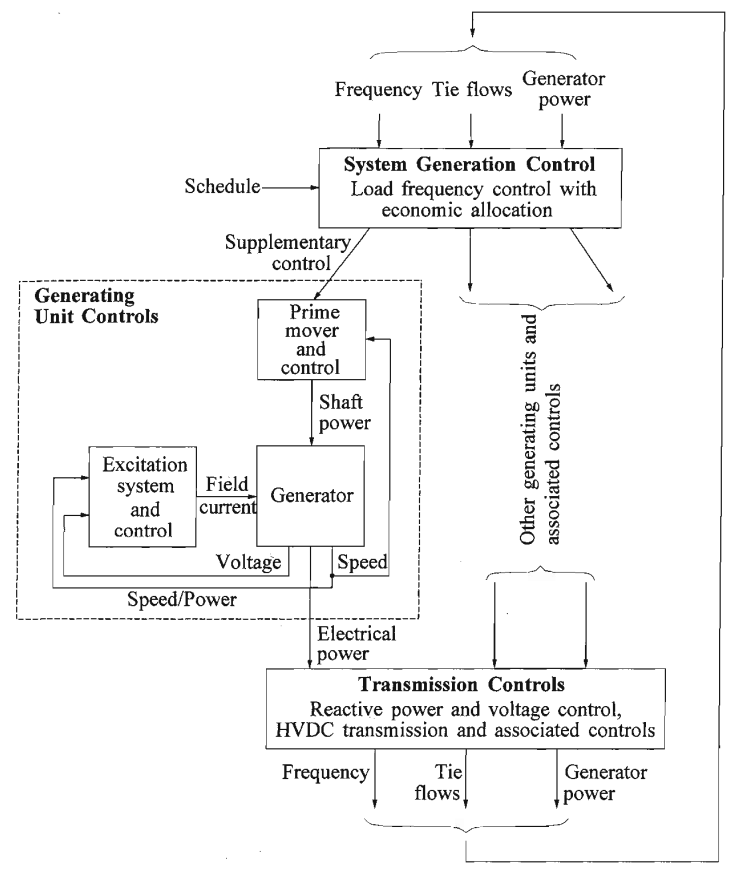
\includegraphics[scale=0.4]{controllo_generico}
	\caption{Struttura generale del controllo di un power system}
	\end{figure}
	\subsection{Sistema d' eccitazione e AVR}
	\begin{figure}
		\centering
		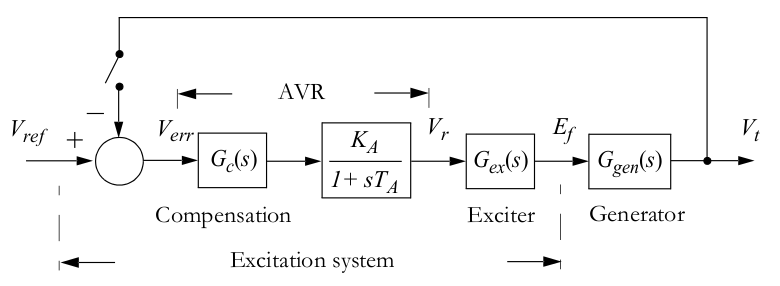
\includegraphics[height=0.20\textheight]{AVR}
		\caption{AVR e sistema d' eccitazione}
	\end{figure}
	Il sistema d' eccitazione è l' apparato che produce la tensione sul circuito di rotore, e, come già accennato è sede dell' AVR e del PSS. Il sistema è costituito da un insieme di dispositivi complessi, che non andremo ad affrontare nel dettaglio. Infatti in linea generale è possibile considerare delle funzioni di trasferimento equivalenti di cui conosciamo i parametri che sono forniti dai produttori (figura 3.2).\\
	Il ruolo dell' AVR è quello di produrre un segnale di tensione regolato sulla base dell' errore generato dalla differenza tra la tensione di riferimento e la tensione registrata sullo statore. Questo segnale va in ingresso al blocco d' eccitazione, che produrrà quindi la $E_{fd}$, che va in ingresso al generatore. Sulla base della figura di sopra, si capisce come $G_{gen}(s)$ sia proprio la funzione di trasferimento $\frac{V_t(s)}{E_{fd}(s)}$; essendo però la macchina sincrona un sistema MIMO è chiaro che nel tuning dell' AVR non vengono considerate le altre variabili di stato, ed è proprio per questo motivo che l' AVR tendenzialmente diminuisce la stabilità della macchina, producendo oscillazioni abbastanza frequenti della $\omega$, ma soprattutto influisce sulla stabilità dell' angolo di rotore, poiché non tiene conto degli effetti che la regolazione di tensione ha sui vari $\delta_i$. E' proprio per questo che esiste un altro controllore, il PSS, che serve appunto ad aumentare la stabilità. La relazione tra PSS e AVR è chiaramente visibile in figura 3.3. Sulla base di $\omega$ esso produce un segnale di tensione $V_s$ che si aggiunge alla tensione registrata e che va in ingresso all' AVR.\\
	Quest' ultimo è formato da un blocco di compensazione $G_c(s)$ e da un blocco di amplificazione $\frac{K_a}{1+\tau_as}$. In questo lavoro si determineranno i parametri del blocco di compensazione, ed essendo l' amplificatore un dispositivo legato alla progettazione lo si considererà come un elemento già noto da accorpare al plant $G_{gen}$. La compensazione è solitamente fatta o attraverso l' impiego di una legge di controllo di tipo PID, o attraverso un blocco di tipo Transient Gain Reduction (TRG), che si basa sull' impiego di reti compensatrici che spostano i poli del plant verso sinistra, così da determinare transitori più rapidi. La scelta fatta in questo lavoro è quella di usare un controllore di tipo PID, quindi si avrà una relazione tra errore ($e(s)$) e tensione regolata ($V_r(s)$) del tipo:
	\begin{figure}
		\centering
		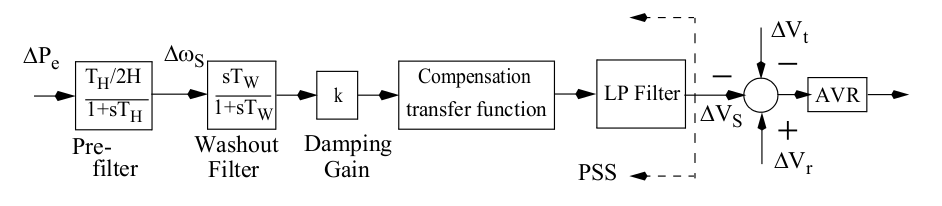
\includegraphics[height=0.13\textheight]{PSS}
		\caption{Schema generico PSS}
	\end{figure}
	\begin{equation*}
	V_r(s)=e(s)(k_p+\frac{k_i}{s}+k_ds)(\frac{k_a}{1+\tau_as})
	\end{equation*}\\
	Poiché il termine derivativo è irrealizzabile, essendo una funzione di trasferimento impropria, si utilizza un' approssimazione ingegneristica della legge di controllo derivativa, che appunto viene filtrata in banda attraverso il parametro N, ottenendo una relazione tra $E_{fd}(s)$ e l' errore $e(s)$:\\
	\begin{equation*}
	\frac{E_{fd}(s)}{e(s)}=(k_p+\frac{1}{T_is}+\frac{T_ds}{1+\frac{T_d s}{N}})(\frac{k_a}{1+\tau_as})G_{ex}(s)=(k_p+\frac{1}{T_is}+\frac{T_ds}{1+\frac{T_d s}{N}})(\frac{k_a}{1+\tau_as})(\frac{k_e}{1+\tau_es})
	\end{equation*}
	Resta ora solo da capire come identificare la funzione di trasferimento del plant, cioè $\frac{V_t(s)}{E_{fd}(s)}$. Guardando il modello con lo spazio di stato si hanno a disposizione come variabili di stato le tensioni in diretta e quadratura $E_d$ e $E_q$ delle varie macchine. L' obiettivo è sempre quello di lavorare nel dominio di Park, per non dover gestire funzioni sinusoidali del tempo, e quindi lavoreremo sul modulo del vettore $E_t$, che è il vettore avente per componenti $E_d$ e $E_q$, pertanto il suo modulo è pari a:
	$|E_t|=\sqrt{E_d^2+E_q^2}$. La relazione tra $E_t$ e le tensioni in diretta e quadratura quindi non è lineare, ma visto che stiamo lavorando su un modello linearizzato, non bisogna dimenticarsi che stiamo parlando di variazioni di grandezze, quindi possiamo approssimare la relazione al primo ordine:\\
	\begin{equation*}
	E'_t=\frac{\partial E_t}{\partial E'_q}E_q+\frac{\partial E'_t}{\partial E'_d}E'_d= \frac{E'_{d0}}{E'_{t0}}E_d+\frac{E'_{q0}}{E'_{t0}}E'_q
	\end{equation*}
	Di conseguenza, data la relazione lineare che sussiste tra le variabili, è possibile scrivere:
	\begin{equation}
	\frac{E'_t(s)}{E_{fd}(s)}=\frac{E'_{d0}}{E'_{t0}}\frac{E'_d(s)}
	{E_{fd(s)}}+\frac{E'_{q0}}{E'_{t0}}\frac{E'_q(s)}{E_{fd}(s)}\\
	\end{equation}
	Con i dati in figura 2.9, sviluppando i calcoli e ricordando che per come è stato sviluppato il modello non siamo interessati a indagare sui controllori della macchina 1, si ottiene:\\
	\begin{equation*}
	\begin{cases}
	\frac{E'_{t2}}{E_{fd2}}=-\frac{0.6940}{1.050188}\frac{E'_{d2}(s)}{E_{fd2}(s)}+\frac{0.7882}{1.050188}\frac{E'_{q2}(s)}{E_{fd2}(s)}\\
	\frac{E'_{t3}}{E_{fd3}}=-\frac{0.6668}{1.017}\frac{E'_{d3}(s)}{E_{fd3}(s)}+\frac{0.7679}{1.018}\frac{E'_{q3}(s)}{E_{fd3}(s)}
	\end{cases}
	\end{equation*}
	Considerando le precedenti relazioni è possibile riportare il modello su Simulink (pagina seguente).
	\begin{figure}
		\centering
		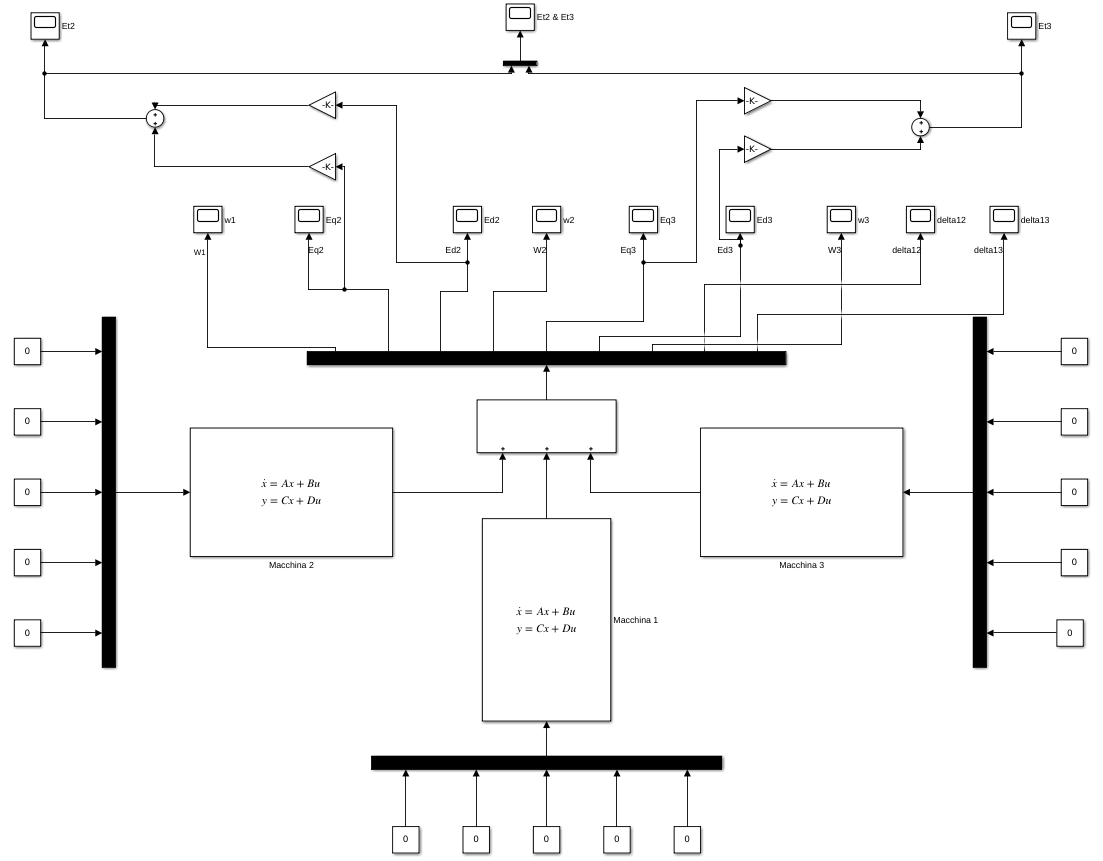
\includegraphics[height=0.6\textheight,angle=-90]{Macchina_non_regolata}
		\caption{Modello della rete in assenza di controllori}
	\end{figure}
\newpage	
	In questo lavoro ci concentreremo sul controllo delle tensioni $E'_{t2}$ e $E'_{t3}$, agendo sulle variabili controllate $E_{fd2}$ e $E_{fd3}$. Per iniziare esaminiamo la risposta delle tensioni in uscita a un ingresso a gradino delle tensioni di field delle macchine 2 e 3 (figura 3.5). I gradini in ingresso devono avere ampiezza ridotta, essendo in p.u. e trovandoci nel caso di un' analisi per piccoli segnali ci limiteremo a ingressi di ampiezza che varia tra -0.1 e +0.1, che corrispondono a variazioni del 10 percento. E' possibile notare come la risposta a regime del sistema non insegua il riferimento, e che si assesta in un tempo di 30000 p.u. Infatti bisogna ricordare che avendo normalizzato anche il tempo rispetto alla frequenza di rete a regime, la scala temporale è dilatata, infatti:
	\begin{equation}
	\tau=377t \rightarrow t=\frac{\tau}{377}
	\end{equation}
	\subsection{Tuning del blocco di compensazione}
	Per questioni di spazio, è stata determinata la funzione di trasferimento $\frac{E_{ti}(s)}{E_{fdi}(s)}$ per $i=2,3$, ed è stato effettuato lo studio in due modelli separati. Si procederà col riportare nel dettaglio i passaggi effettuati per il tuning del PID sulla macchina 2, e vista la similarità del procedimento per effettuare lo stesso sulla macchina 3, di quest' ultima verranno riportati i dati finali.
	Per prima cosa dobbiamo determinare i parametri, dell' amplificatore (amplifier2) e dell' eccitatore (exciter2) della macchina 2, che sono in figura 3.6.
	\begin{figure}
	\centering
	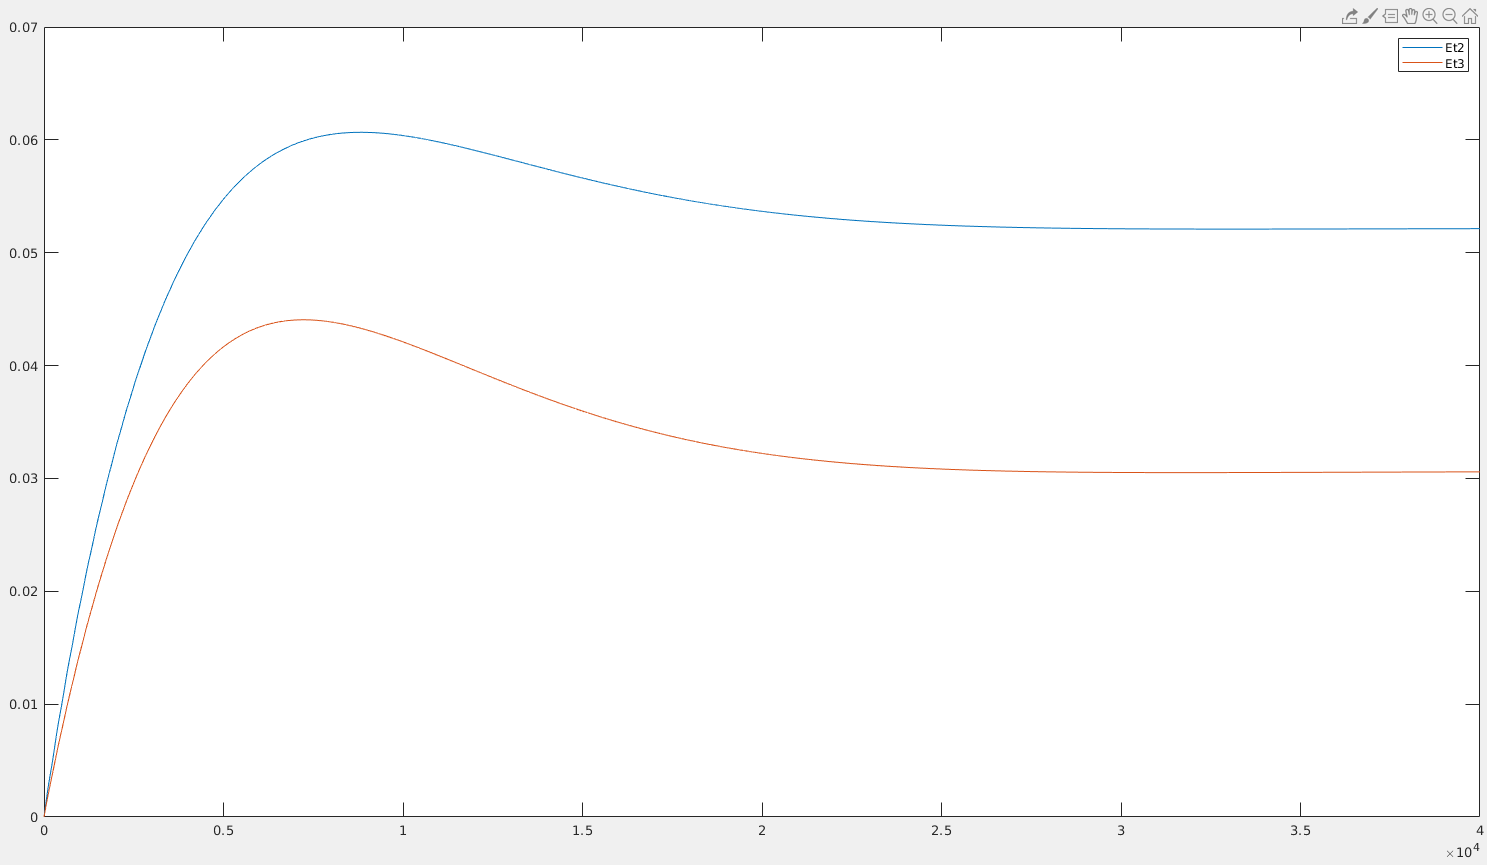
\includegraphics[height=0.35\textheight]{Sistema_non_regolato}
	\caption{Uscita non regolata ad uno step di 0.07 (macchina 2) e 0.05 (macchina 3)}
	\end{figure}	
	\begin{figure}
	 	\centering
	 	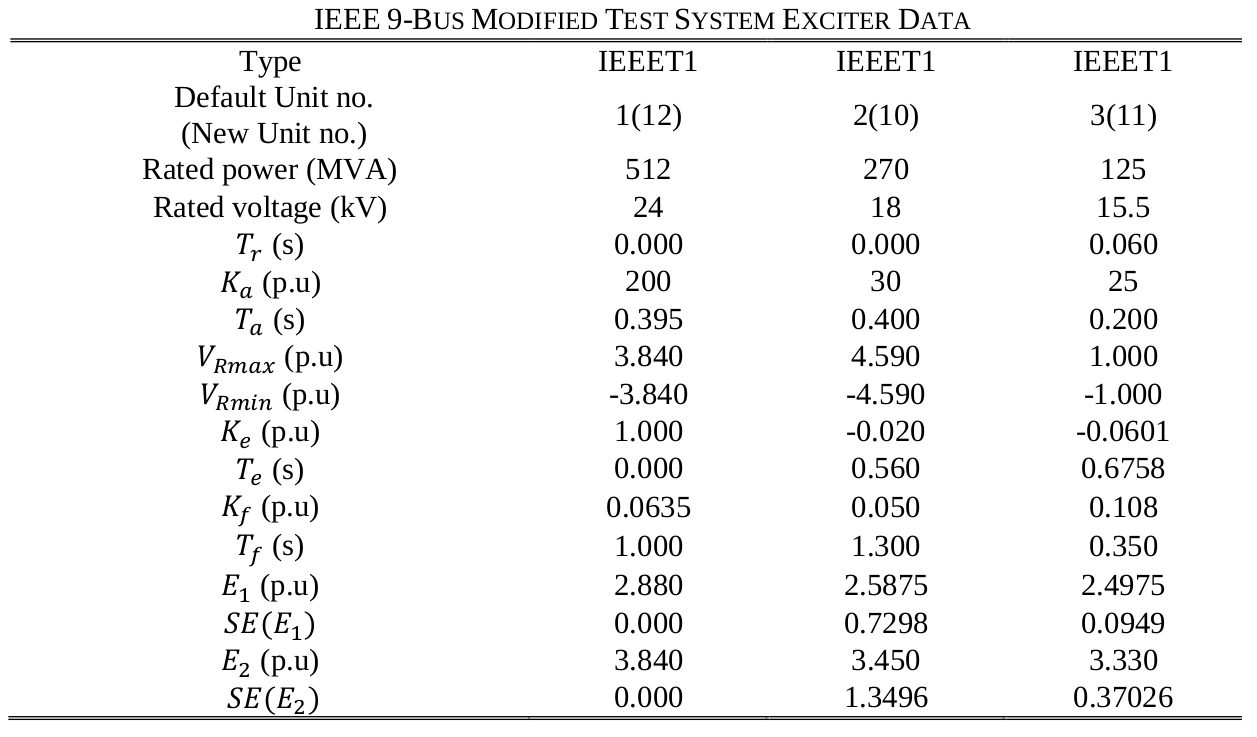
\includegraphics[height=0.3\textheight]{Dati_Sistema_Eccitazione}	 	\caption{Dati del sistema di eccitazione delle varie macchine}
	\end{figure}
 	E' importante notare che le unità di misura delle costanti di tempo in tabella sono riportate in secondi, quindi non normalizzate. \\\\\\\\Per inserire questi blocchi nel nostro modello è opportuno normalizzarle secondo l' equazione 2.8, e quindi avremo:\\ $\text{amplifier}_2(s)=\frac{k_a}{1+\tau_as}=\frac{30}{1+150.8s}$ \qquad $\text{exciter}_2(s)=\frac{k_e}{1+\tau_es}=\frac{-0.02}{1+211.1s}$.
 	Seguendo lo schema in figura 3.2 quindi la funzione di trasferimento a valle del PID è:\\
 	$P_2=\text{amplifier}_2(s)\cdot\text{exciter}_2(s)\cdot\frac{E_{t2}(s)}{E_{fd2}(s)}$. $\text{P}_2$ è una funzione a 17 poli a parte reale negativa:\\
 	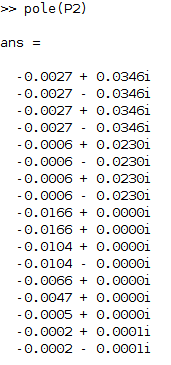
\includegraphics[height=0.26\textheight]{poli_p2}\\
 	Ciò vuol dire che per spostare arbitrariamente a sinistra i poli nel piano complesso, per determinare transitori esigui, servirebbe un controllore di ordine 17, che è molto costoso. Il PID invece è un controllore di ordine 2, che può essere tarato seguendo delle regole e fornisce un controllo abbastanza soddisfacente in molte situazioni. In questo lavoro si procederà attraverso l' impiego di vari metodi di sintesi del PID. Per fare ciò però c'è bisogno di riportare la funzione di trasferimento del plant a 17 poli ad un blocco ad un solo polo che approssima maggiormente la risposta di P2 a un ingresso a gradino.\\
 	La funzione di trasferimento approssimata deve essere del tipo:\\
 	$\frac{K}{1+T_1 s} e^{-\tau s}$, dove $e^{-\tau s}$ è un fattore di ritardo.\\\\\\\\\\Per far ciò si utilizzerà un tool di stima della risposta a gradino presente nel toolbox di System Identification di Matlab, il cui risultato è riportato in figura 3.7.
 	\begin{figure}
 		\centering
 		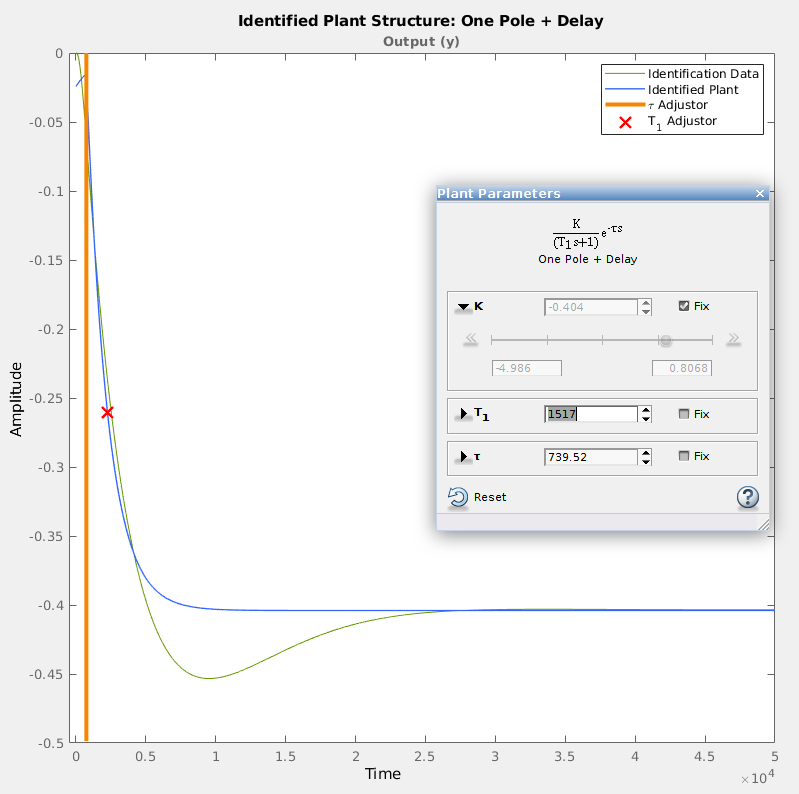
\includegraphics[scale=0.45]{P2_estimating1}
 		\caption{Stima del processo $P_2$}
 	\end{figure}
	La funzione di trasferimento è quindi:\\
	$P2=-\frac{0.404}{1+1517.4s}e^{-739.52s}$\\\\\\
	Ora non rimane che seguire le regole di sintesi del PID, che sono riportate in figura 3.8.
	\begin{figure}
		\centering
		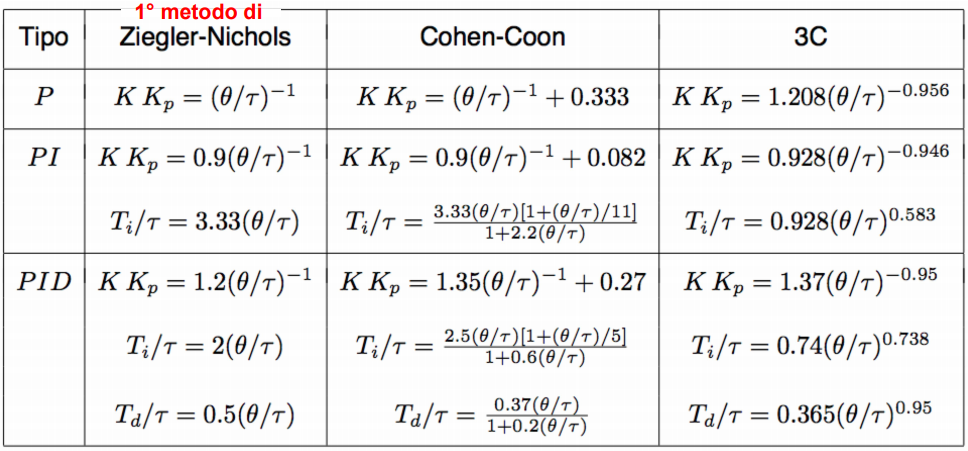
\includegraphics[height=0.27\textheight,]{Regole_PID}
		\caption{Regole euristiche di sintesi del PID}
	\end{figure}
	Attraverso l' uso della funzione "tuning\textunderscore migliore.m", (appendice A.1) è stato determinato il metodo più efficace, attraverso l' analisi della risposta della funzione ad anello chiuso $W=\frac{\text{PID}(s)\cdot P2(s)}{1+\text{PID}(s)\cdot P2(s)}$,di cui si riporta il risultato in figura 3.8.\\
	Il PID che genera un tempo d' assestamento più breve è
	quello sintetizzato con il metodo di Cohen-Coon.
	\begin{figure}
		\centering
		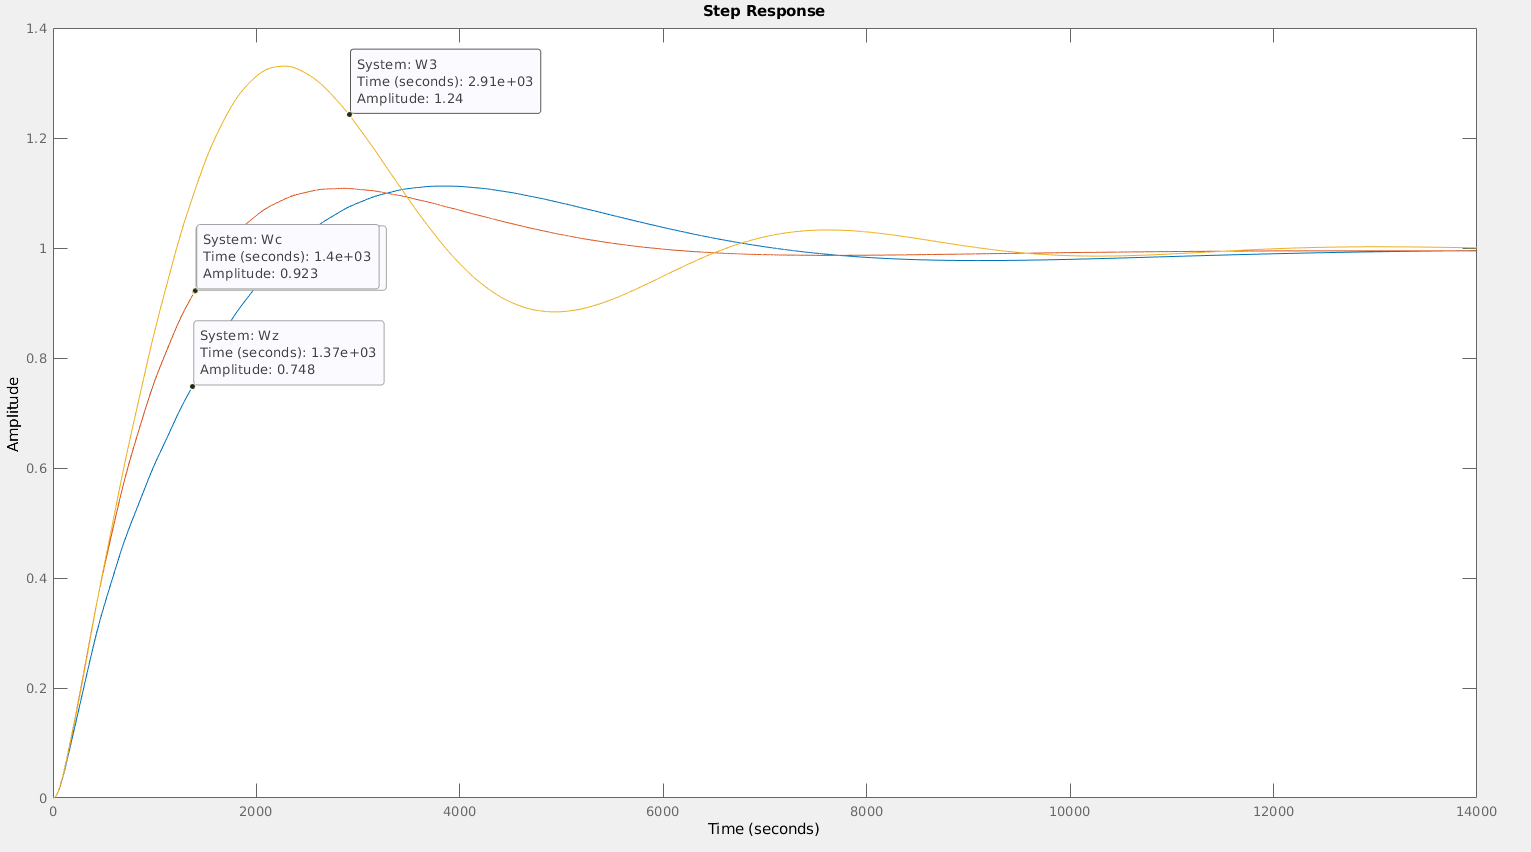
\includegraphics[scale=0.26]{step_response_metodi_P2}
			\caption{Risposta a gradino in base ai vari metodi}
	\end{figure}
	Un altro punto da chiarire è la scelta del filtro in banda dell' azione derivativa N. Pertanto è stata scritta un' altra funzione, "seleziona\textunderscore N.m" (appendice A.2), che grafica le varie risposte del sistema al variare di N (figura 3.10).
	\begin{figure}[h]
		\centering
		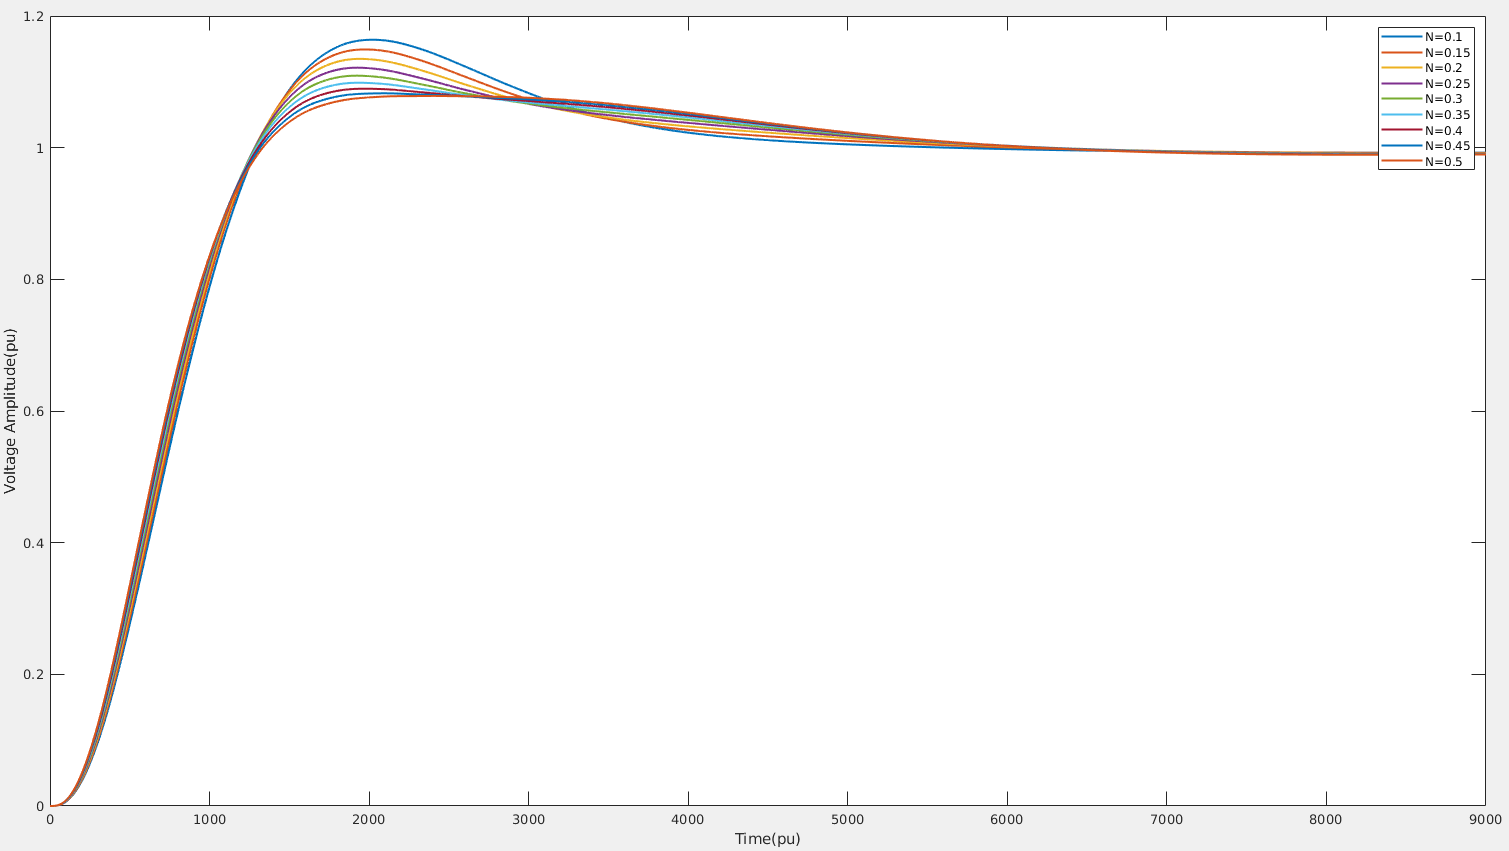
\includegraphics[height=0.33\textheight]{vari_N}
		\caption{Risposta a gradino al variare di N}
	\end{figure}E' stato scelto il valore di N che genera un tempo d' assestamento minore, quindi $N=0.1$.
	La scelta della funzione di trasferimento del PID effettuata in due step successivi potrebbe indurre a pensare che il variare di N potrebbe appunto modificare in maniera determinante le risposte con l' utilizzo dei vari PID, quindi è stata scritta la funzione "tuning\textunderscore selezionaN.m" (appendice), che determina il minor tempo d' assestamento al variare sia del metodo di tuning del PID sia del filtro in banda.Si riporta il risultato qui in basso:\\
	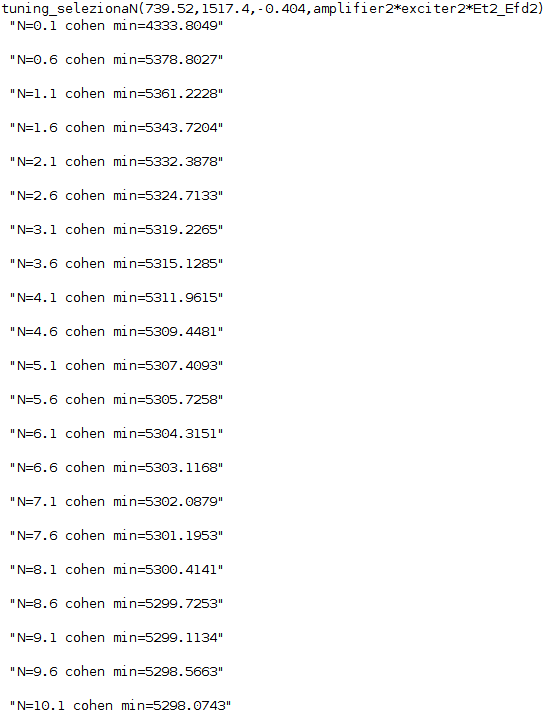
\includegraphics[scale=0.5]{tuning_selezionaN_P2} \\\\
	Si vede che il metodo di Cohen-Coon genera sempre il tempo d' assestamento minore rispetto agli altri metodi, e in particolare lo si ha per N=0.1.\\
	Con questa scelta si ottiene la funzione di trasferimento del PID:
	\begin{equation*}
	PID_2=\frac{-2064s^2-19.47s-0.004793}{2493s^2+s}
	\end{equation*}
	Lavorando in per-unit è opportuno chiedersi se la funzione di trasferimento da origine a valori di guadagni e costanti di tempo che hanno effettivamente senso. Utilizzando la funzione "trova\textunderscore parametri.m" (appendice A.3), è possibile trovare i corrispettivi valori di $k_p$,$T_i$,$T_d$. In questo caso si ha:\\
	\[
	\begin{cases}
	k_p=-7.5248\\
	T_i=1569.9 \quad\text{pu}=4.1641\quad s\\
	T_d=249.3206\quad \text{pu}=0.66\quad s
	\end{cases}
	\]
	L' AVR in letteratura può essere arricchito da un ulteriore guadagno $K_g$, e quindi ha senso chiedersi se è possibile migliorare la disposizione dei poli della funzione ad anello chiuso includendo questo ulteriore guadagno $K_g$. Questo può essere verificato utilizzando il luogo delle radici, di cui si riportano i grafici qui di seguito (luogo positivo in alto, negativo in basso).\\\\
	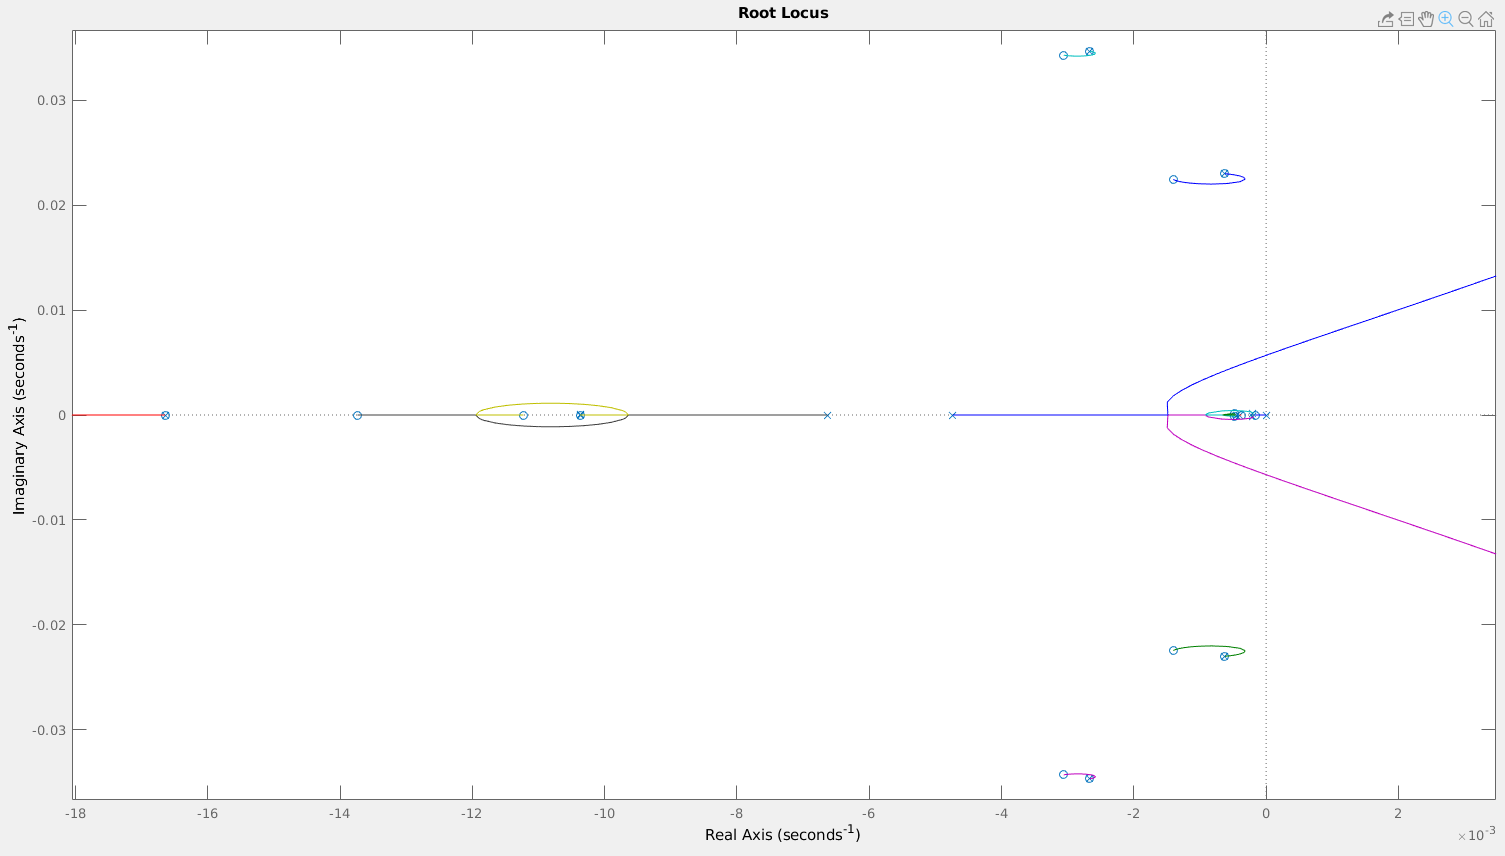
\includegraphics[scale=0.27]{rlocus_P2_pos}\\
	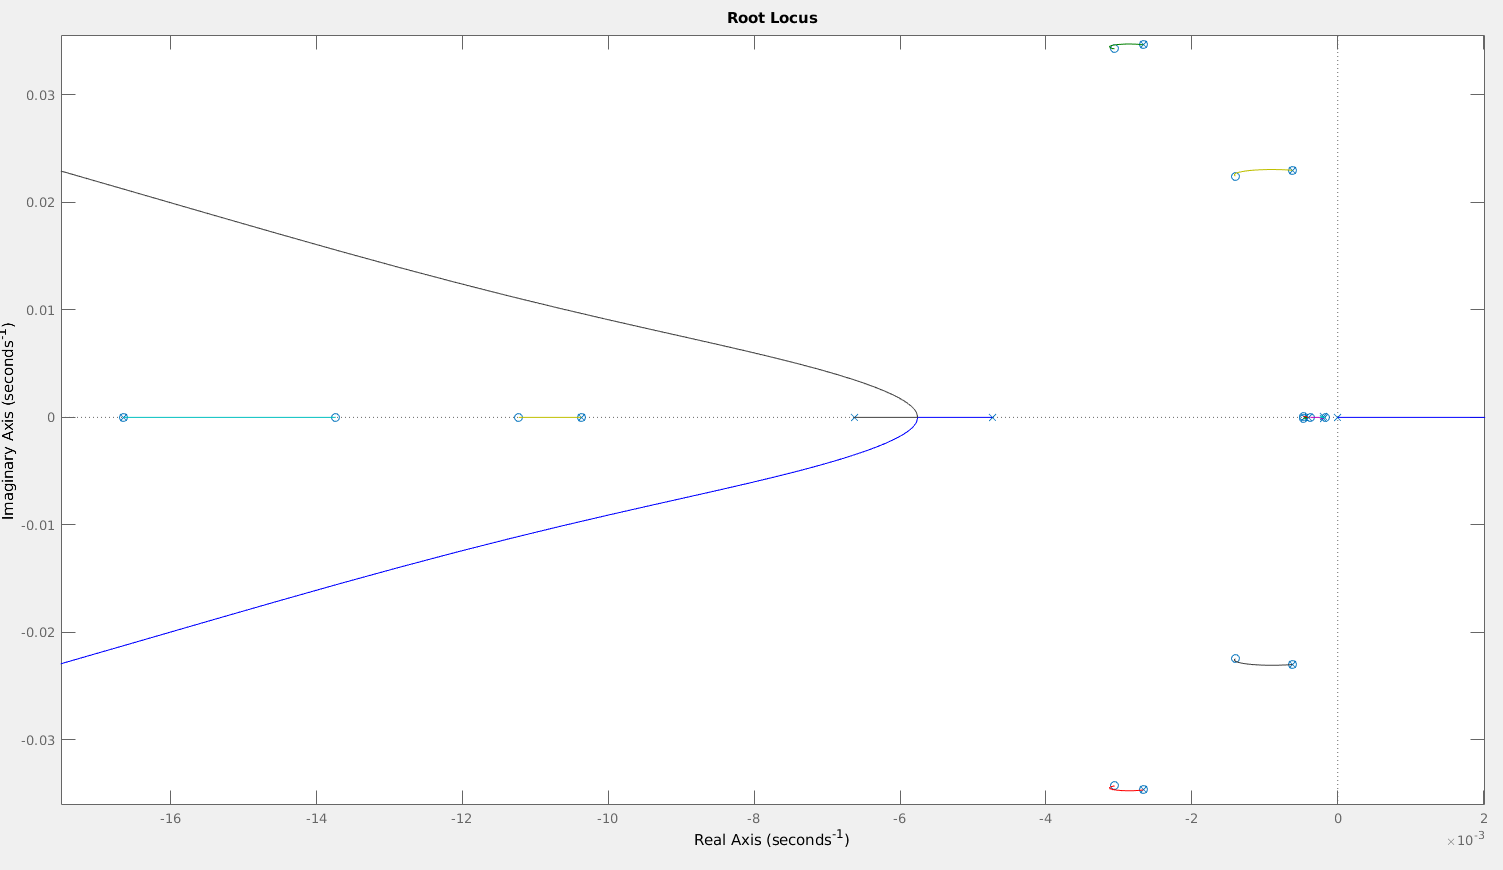
\includegraphics[scale=0.27]{rlocus_P2_neg}\\\\
	Possiamo notare come la scelta di un $K_g$ negativo porti il polo nell' origine (corrispondente all' inserimento dell' azione integrale) a muoversi nel semipiano positivo, generando instabilità. Per quanto riguarda il luogo positivo osserviamo che è possibile aumentare il guadagno senza generare instabilità fino a un valore di $K_g=8$, valore per il quale i due poli (linea viola e fucsia) entrano nel semipiano positivo. In questo range non c'è una significativa differenza nella posizione dei poli. Il polo più estremo a sinistra continua a muoversi in quella direzione, ma non è il polo dominante. Siamo interessati a spostare i poli con modulo della parte reale più piccolo, poiché come sappiamo sono loro che determinano i transitori più lunghi. E' evidente però che l' aumento del guadagno provocherebbe soltanto delle oscillazioni più significative, proprio per il movimento nei poli nella direzione dell' asse immaginario,che degraderebbero le prestazioni dinamiche del sistema.
	Nella pagina seguente vi è un dettaglio del luogo positivo ($0\le K_g\le 1$), che mette in luce come un guadagno di 0.713 conferisca una configurazione dei poli migliore. Infatti si vede come alcuni dei poli complessi coniugati si spostino sull' asse reale, diminuendo così la sovraelongazione nei transitori. E' ovvio però che un guadagno minore porta a un aumento del tempo d' assestamento, e proprio per questo bisogna valutare i pro e i contro di un cambiamento in questo senso.\\
	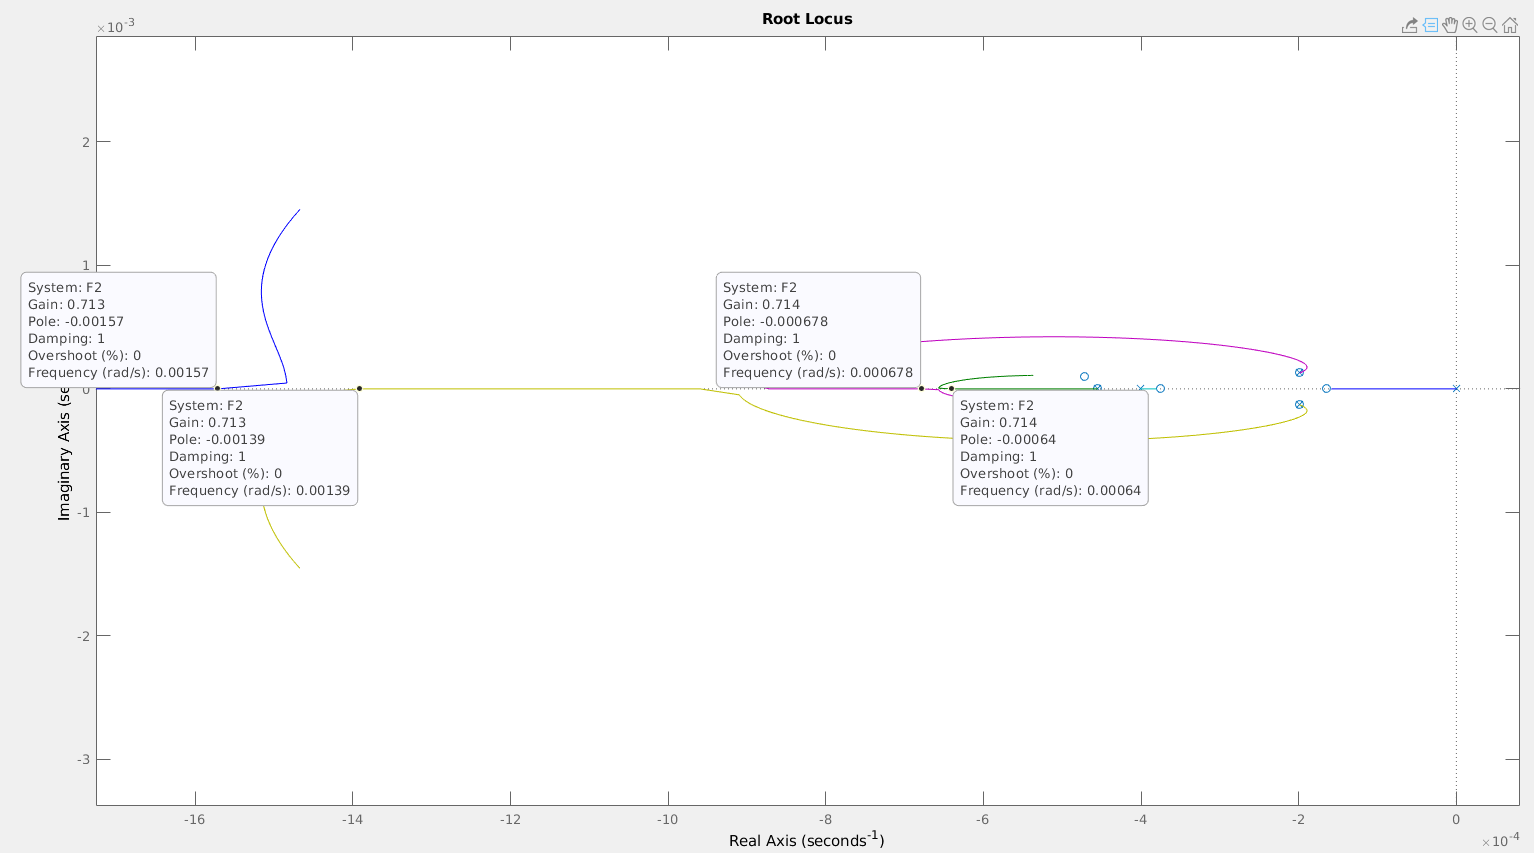
\includegraphics[scale=0.42,angle=90]{rlocus_F2_particolare}\\
	Nell' immagine di sotto la curva in blu rappresenta il sistema con $K_g=1$, quindi inalterato, mentre la curva in rosso rappresenta la risposta del sistema con $K_g=0.713$. E' immediato constatare che nel secondo caso viene diminuita la velocità di risposta del sistema, determinando così un tempo d' assestamento più elevato, il che è sconveniente. Infatti se prima il tempo d' assestamento era di 4412 pu, nel caso di Kg=0.713 si ha un tempo d' assestamento di 5758 pu. La differenza è di 1346 pu, che equivalgono a 3.57 s, un incremento inaccettabile.\\\\
	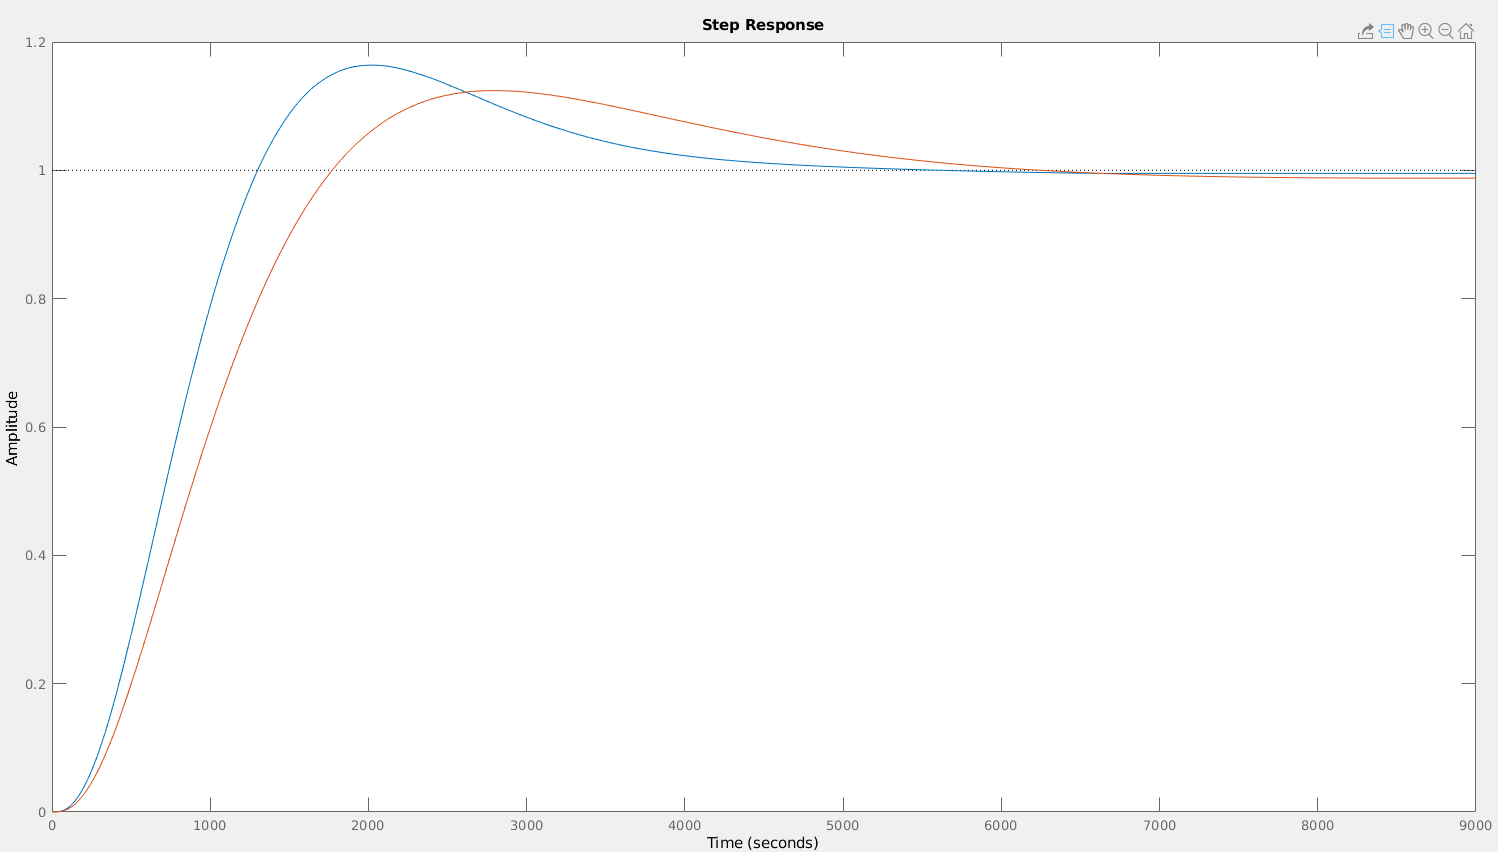
\includegraphics[scale=0.33,angle=90]{step_k_modificato}\\\\
	Siamo ora interessati a vedere i margini di fase e di guadagno del sistema controllato. Si riporta nella pagina seguente il risultato ottenuto utilizzando Matlab.\\\\
	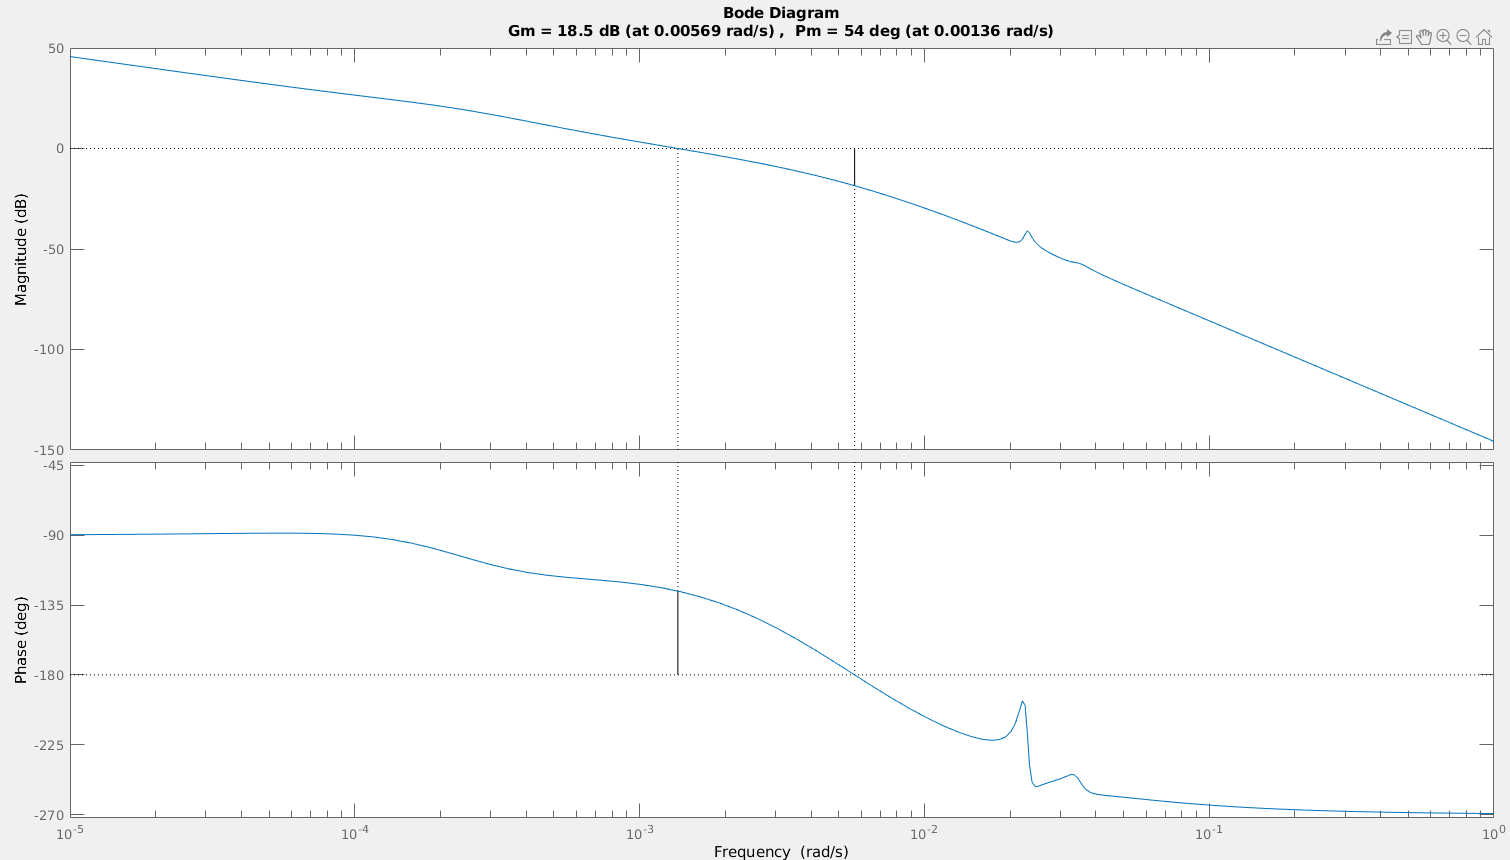
\includegraphics[scale=1.11]{margin_P2}\\\\
	E' possibile vedere che il margine di fase è di 54 gradi e quello di guadagno è di 18.5 dB, valori che sono soddisfacenti per i requisiti di stabilità.\\
	Per quanto riguarda il tuning del PID per l' AVR della macchina 3 il procedimento è lo stesso. Si parte quindi dall' analisi della risposta a gradino del processo $P3=\text{amplifier}_3\cdot\text{exciter}_3\cdot \frac{E'_{t3}(s)}{E_{fd3}(s)}$, e si procede con la stima della stessa con il tool menzionato in precedenza, che viene riportata nella pagina seguente.\vfill
	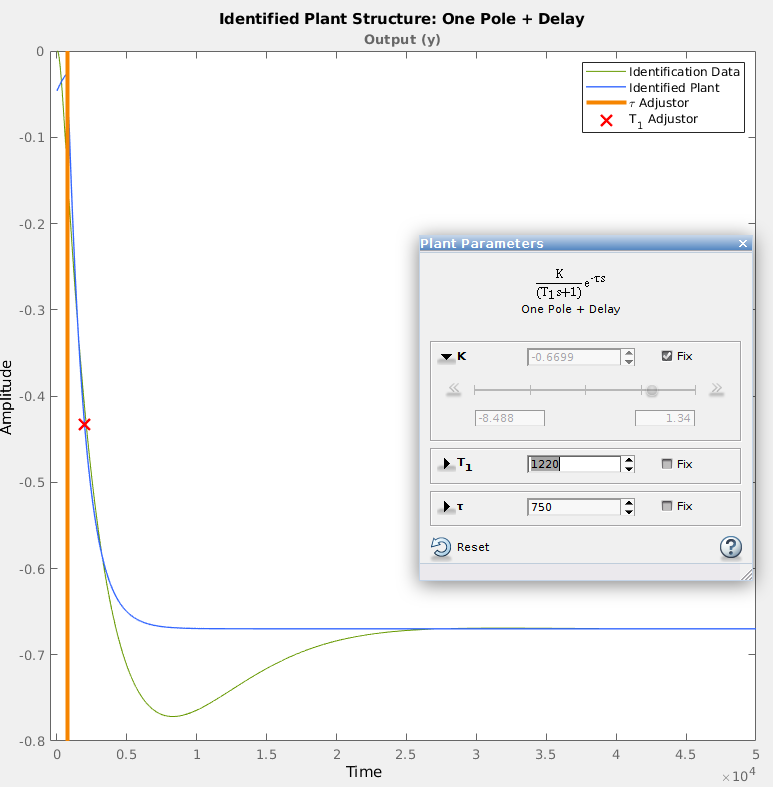
\includegraphics[scale=2]{P3_estimating}\vfill
	La funzione di trasferimento approssimata è dunque:\\
	\begin{equation*}
	P3=\frac{-0.6699}{1+1220s}e^{-634.1s}
	\end{equation*}\\
	Utilizzando le stesse regole di sintesi del PID, e utilizzando di nuovo la funzione per trovare il tuning migliore (risultato a pagina seguente).\\\\
	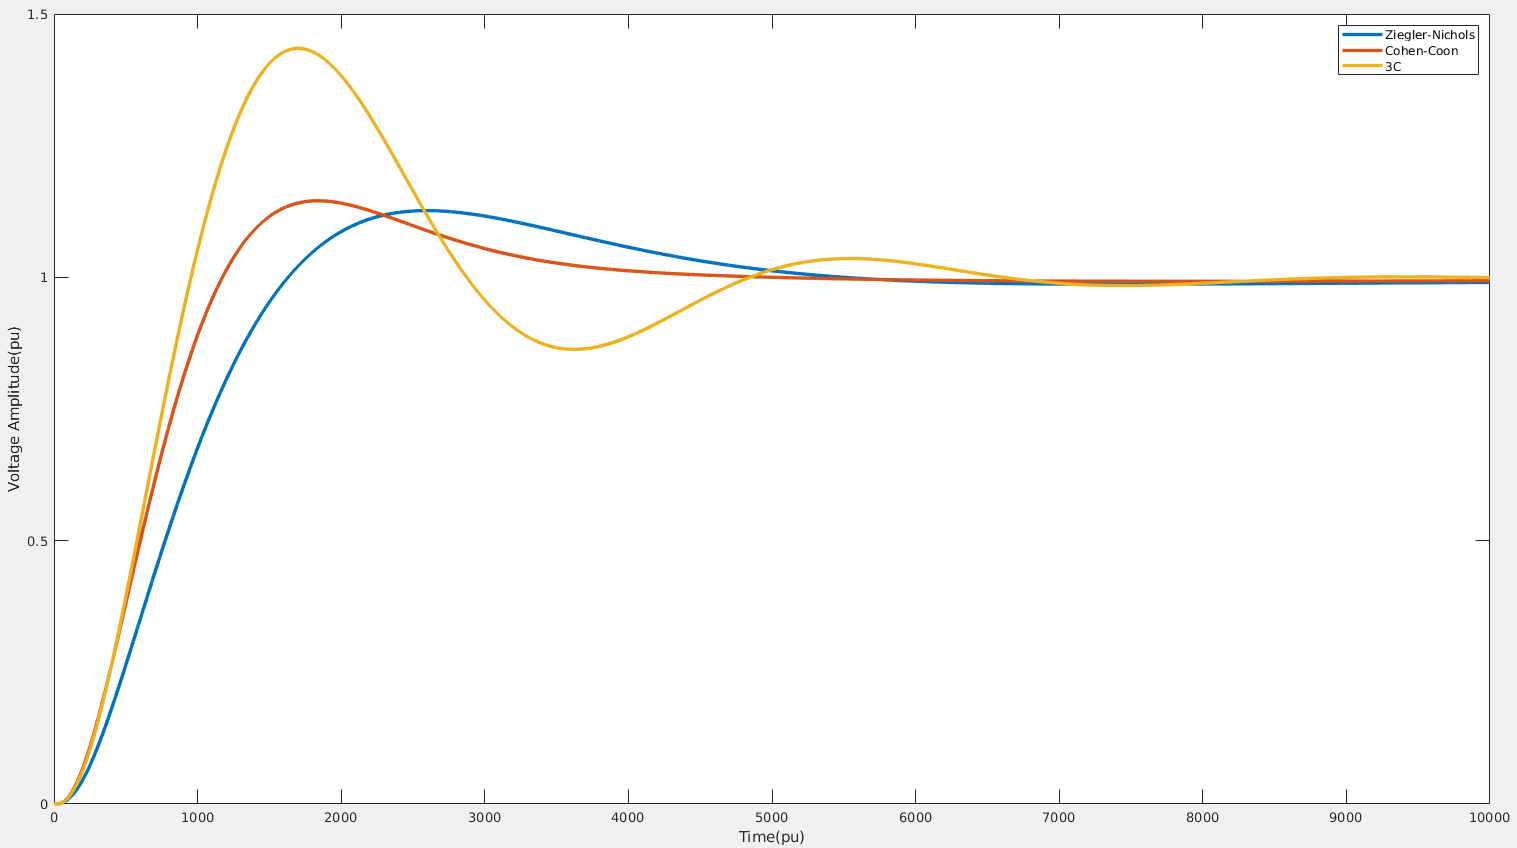
\includegraphics[scale=0.32,angle=90]{tuning_migliore_P3}\\\\
	Verrà quindi usato di nuovo il metodo di Cohen-Coon e scelto il valore di N scegliendo la risposta migliore del sistema controllato tra i grafici sottostanti.\\\\
	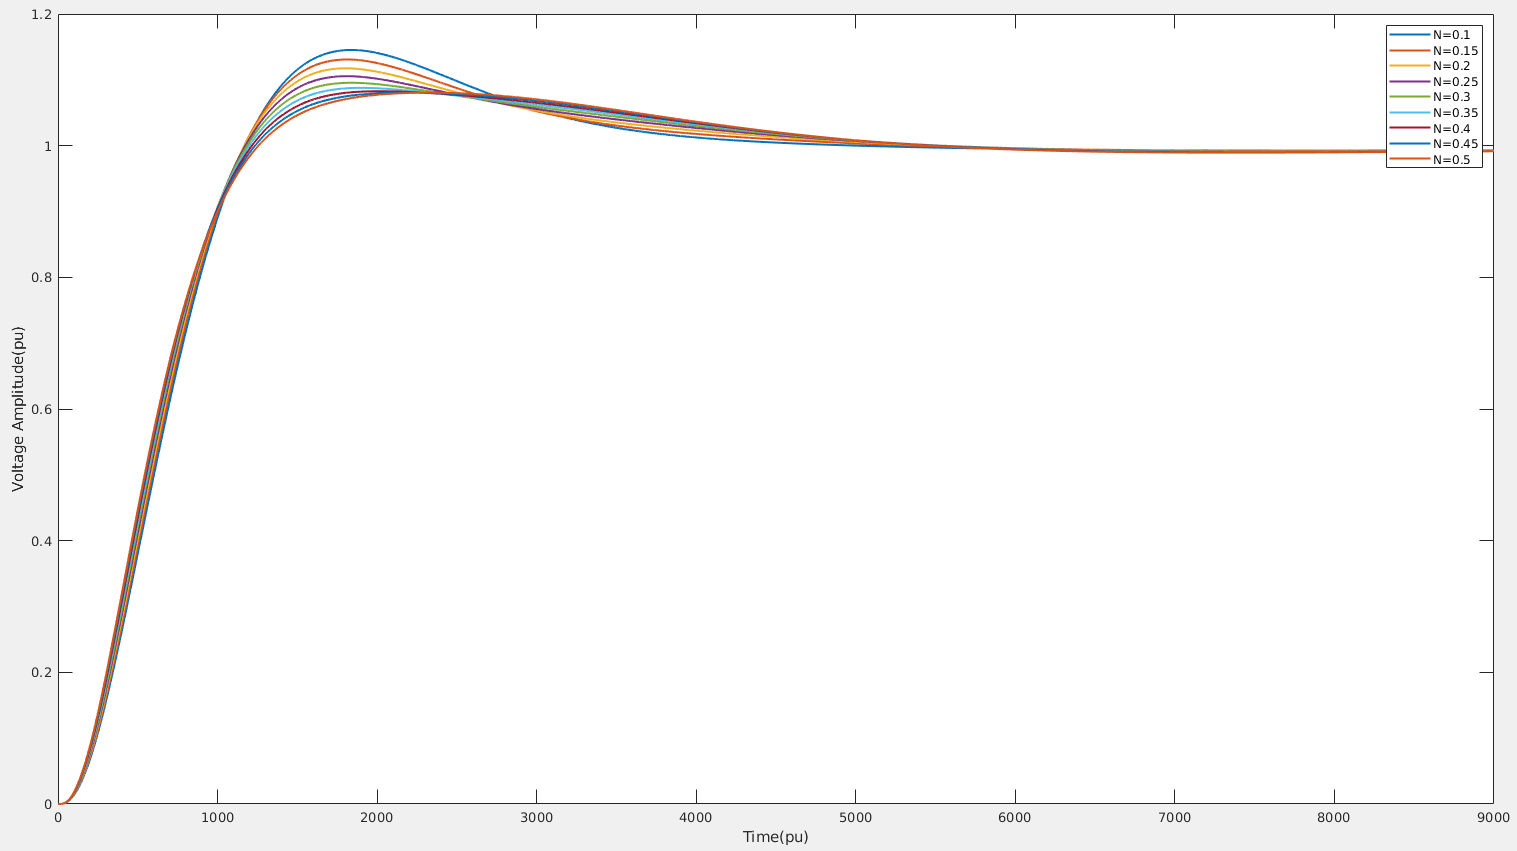
\includegraphics[scale=0.32,angle=-90]{vari_N_P3}\\\\
	La funzione di trasferimento del PID è dunque:\\
	\begin{equation}
	PID_3=\frac{-1001s^2-11.1s-0.003209}{2125s^2+s}\rightarrow\begin{cases}
	k_p=-4.28\\
	T_i=1334 \text{ pu} = 3.538\text{ s}\\
	T_d=212.52 \text{ pu} = 0.5637\text{ s}
	\end{cases}
	\end{equation}\\\\
	Di seguito è riportato il luogo delle radici (positivo in alto e negativo in basso).\\
	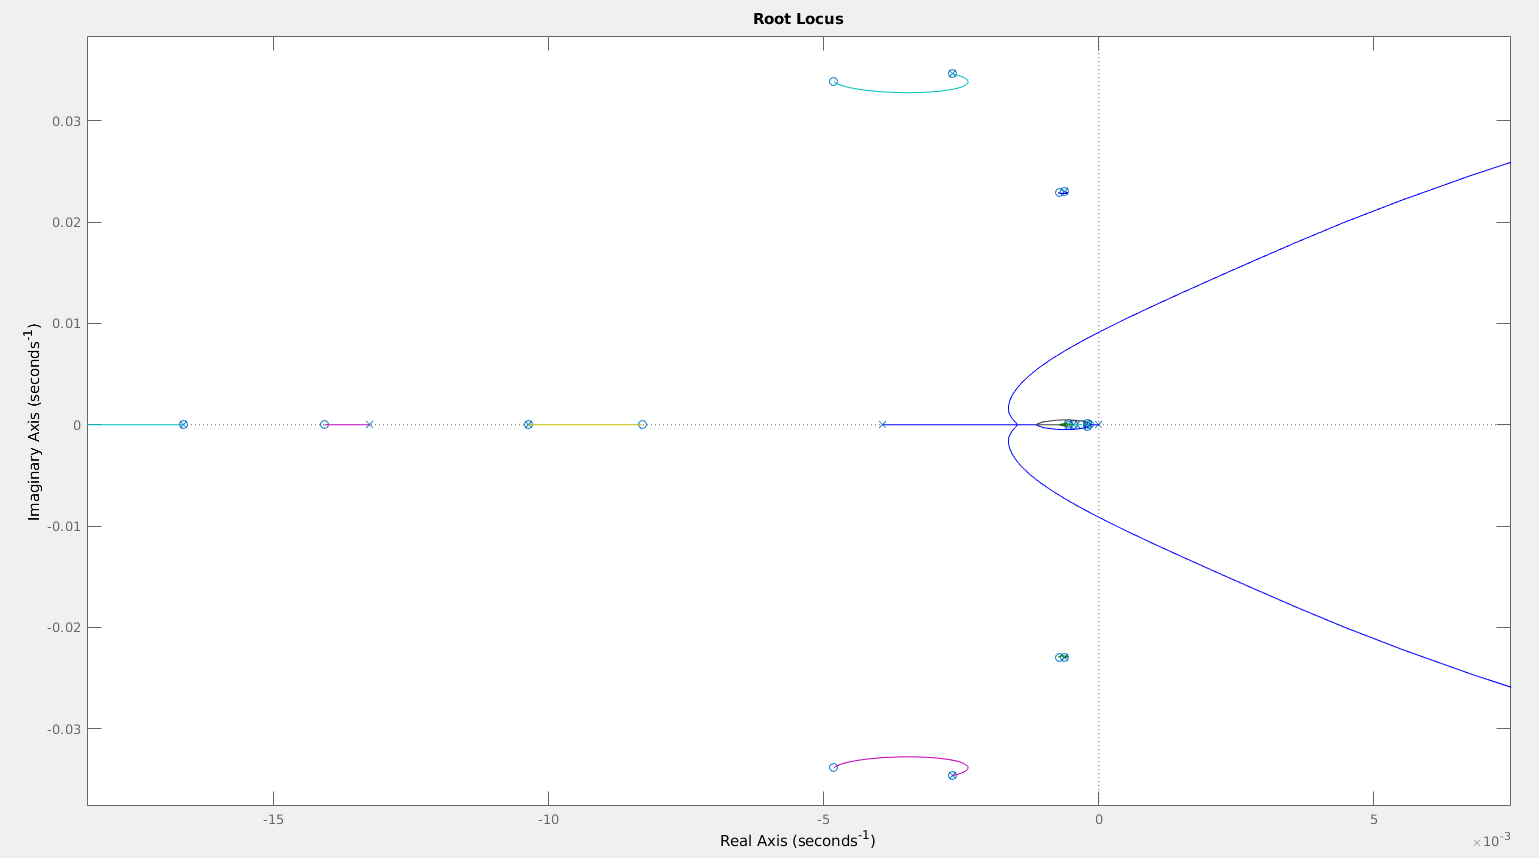
\includegraphics[scale=0.26]{rlocus_F3_pos}\\
	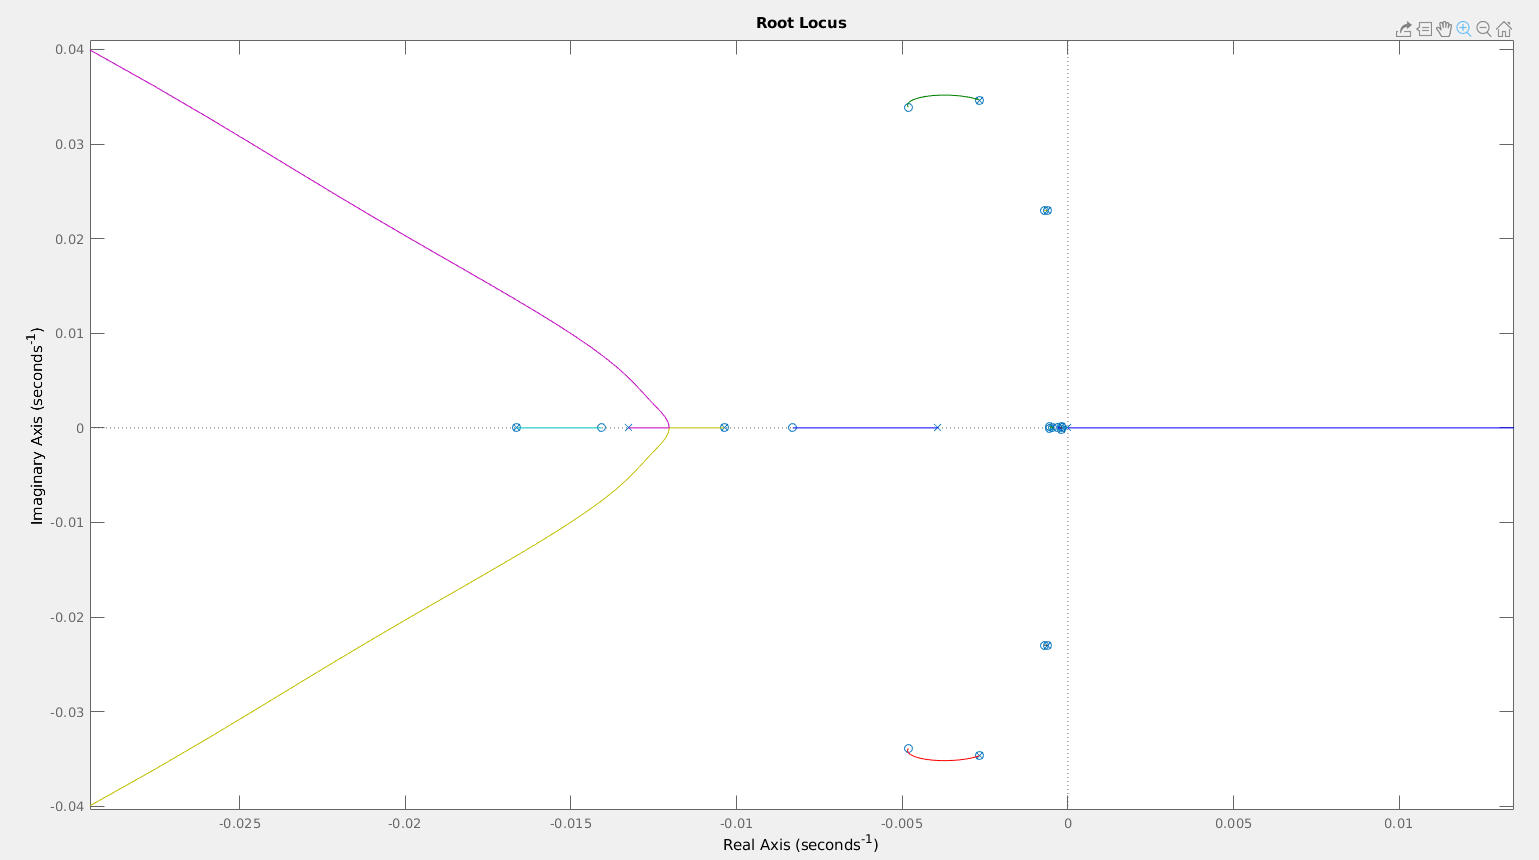
\includegraphics[scale=0.26]{rlocus_F3_neg}\\\\
	Per quanto riguarda il luogo negativo, come nel caso dell' altra macchina, è facile notare che il polo in zero, aumentando il modulo del guadagno, si muoverà verso destra sull' asse reale, generando instabilità. Sappiamo che per ottenere la funzione di trasferimento ad anello chiuso già analizzata in precedenza occorre scegliere un guadagno $K_g=1$; difatti con questa scelta ,se la funzione di trasferimento ad anello aperto è $F_3=PID_3\cdot P_3$, quella ad anello chiuso è $W_3=\frac{F_3}{1+F_3}$. Si è già visto che è sconveniente per i tempi di assestamento indagare su valori di $K_g$ minori di 1. Pertanto scegliendo un vettore di possibili $K_g$ tali che $1\le K_g \le 10$, possiamo esaminare come si spostano i poli guardando la figura sottostante.\\\\
	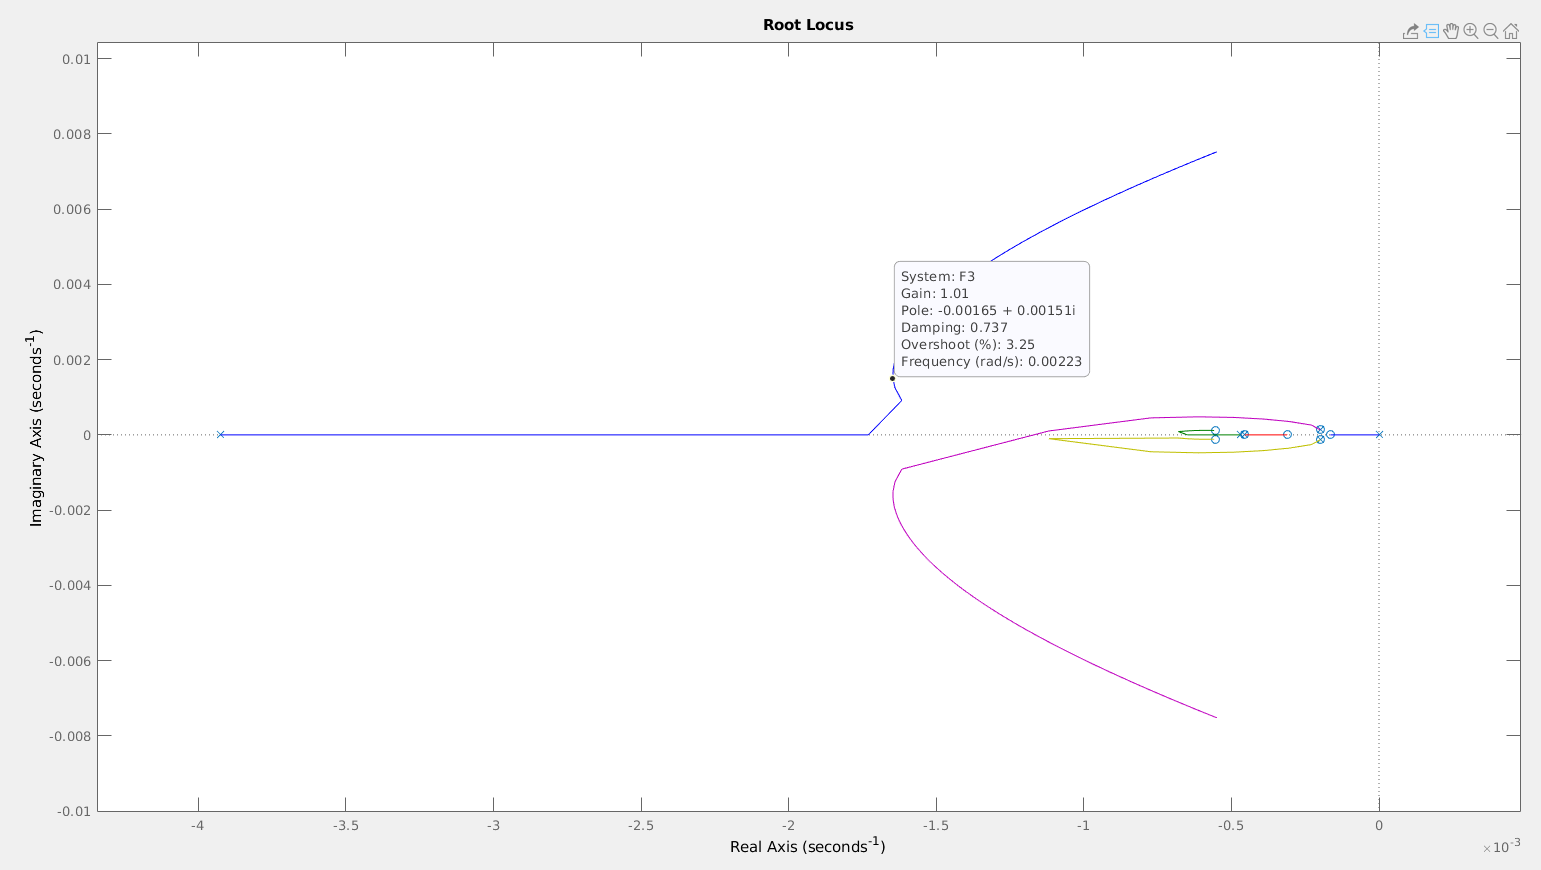
\includegraphics[scale=0.258]{rlocus_F3_particolare}\\\\
	Possiamo vedere come per un guadagno superiore a 1 i poli si muovono nella direzione dell' asse immaginario, generando più oscillazioni nel transitorio, che come già detto, è da evitare. Si riportano i diagrammi di Bode con margine di fase e di guadagno, rispettivamente pari a 56.3 gradi e 23.7 dB.\\\\
	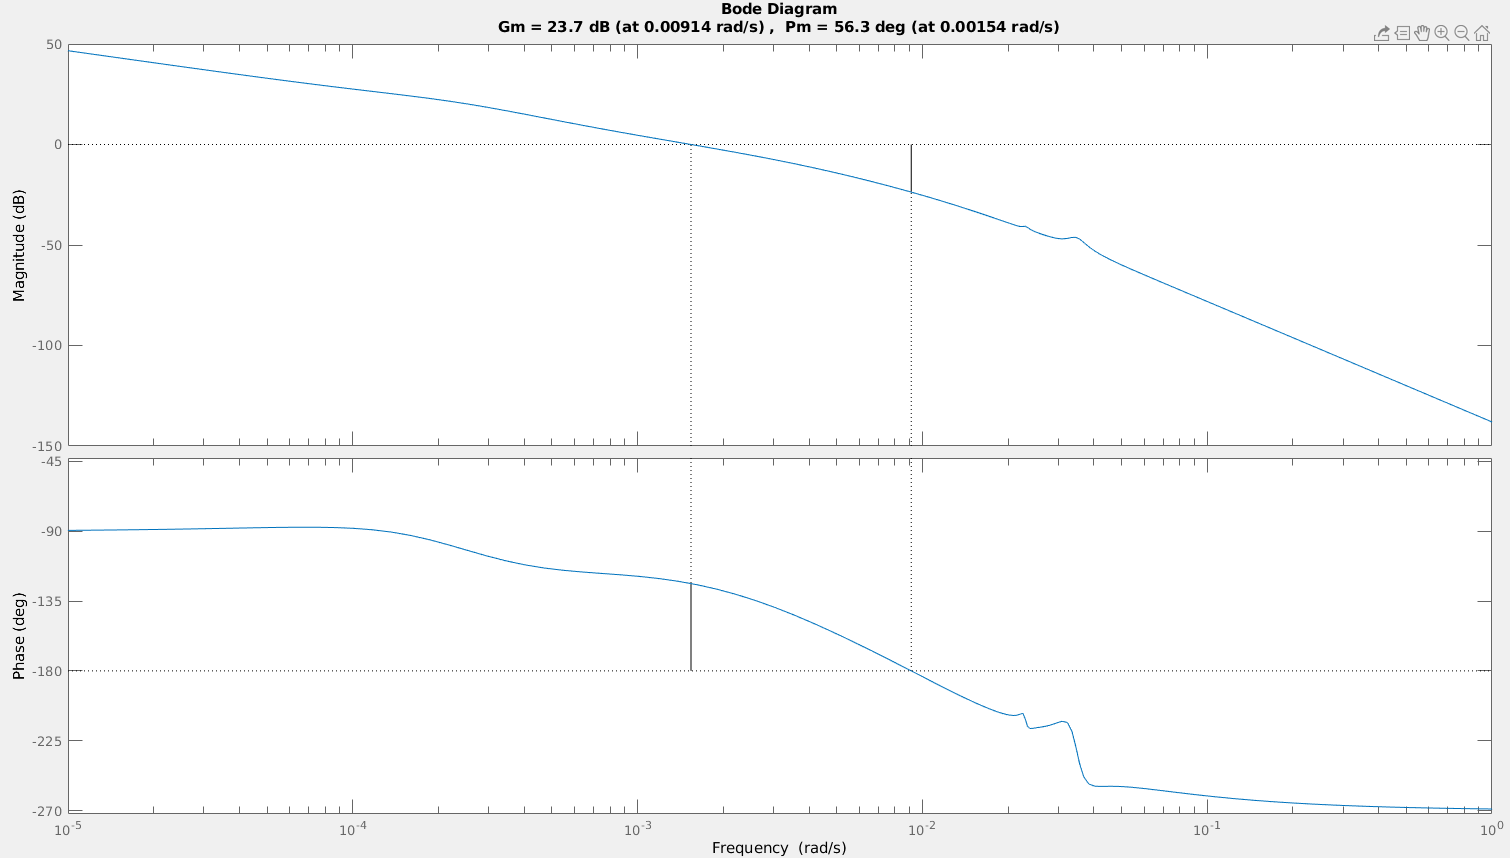
\includegraphics[scale=0.258]{margin_F3}\\\\\\\\\\
	Prima di procedere riportando i blocchi di controllo nello schema generale è opportuno fare alcune precisazioni. Come si comporta il sistema in presenza di disturbi? Difatti si potrebbe pensare di fare un' analisi per piccoli segnali anche in questo senso. Come vengono gestite dai controllori le piccole variazioni delle grandezze elettriche a valle del sistema, oppure rumori modesti in ampiezza dovuti al sistema d' eccitazione stesso? 
	Riferendoci a questa situazione e concentrandoci sulla macchina 2, dato che il ragionamento per la 3 è del tutto analogo:\\
	$E_{t2}(s)=[e(s)\cdot PID(s)\cdot \text{amplifier}_2(s)\cdot \text{exciter}_2(s)+d(s)]\cdot P(s)$\\
	$e(s)=-E_{t2}(s)$\\
	Di conseguenza,\\
	$\frac{e(s)}{d(s)}=-\frac{P(s)}{1+PID\cdot \text{amplifier}_2\cdot \text{exciter}_2\cdot P(s)}$\\
	Ciò vuol dire che l' errore, definito come $-E_{t2}$, va a zero se vi sono disturbi costanti, grazie all' azione integrale del PID. Per avere informazioni sul comportamento dell' uscita $E_{t2}$ in funzione dei disturbi basta considerare sostituire l' espressione di $e(s)$ nella prima equazione ottenendo la relazione precedente ma ovviamente cambiata di segno:\\
	$\frac{E_{t2}(s)}{d(s)}=\frac{P(s)}{1+\text{PID}(s)\cdot \text{amplifier}_2(s)\cdot \text{exciter}_2(s) \cdot P(s)}$\\
	Questa funzione di trasferimento ci da informazioni sulla variabile $E_{t2}$ in funzione dei disturbi. Immaginando questi ultimi come uno step a gradino della forma $d(s)=\frac{d}{s}$ e applicando il teorema del valor finale:\\
	$E_{t2}=sE_{t2}(s)|_{s=0}=s\frac{E_{t2}(s)}{d(s)}\cdot d(s)|_{s=0}=s\frac{E_{t2}(s)}{d(s)}\cdot \frac{d}{s}|_{s=0}=0$.\\
	Il risultato nullo è assicurato dalla presenza dell' azione integrale del PID, e ci dice appunto che dato un disturbo costante l' uscita $E_{t2}$ a regime si assesterà sullo zero, e questo ci assicura una buona reiezione di disturbi costanti. 
	Lo schema a blocchi completo della rete con i controllori annessi è riportato nella pagina seguente.\\
	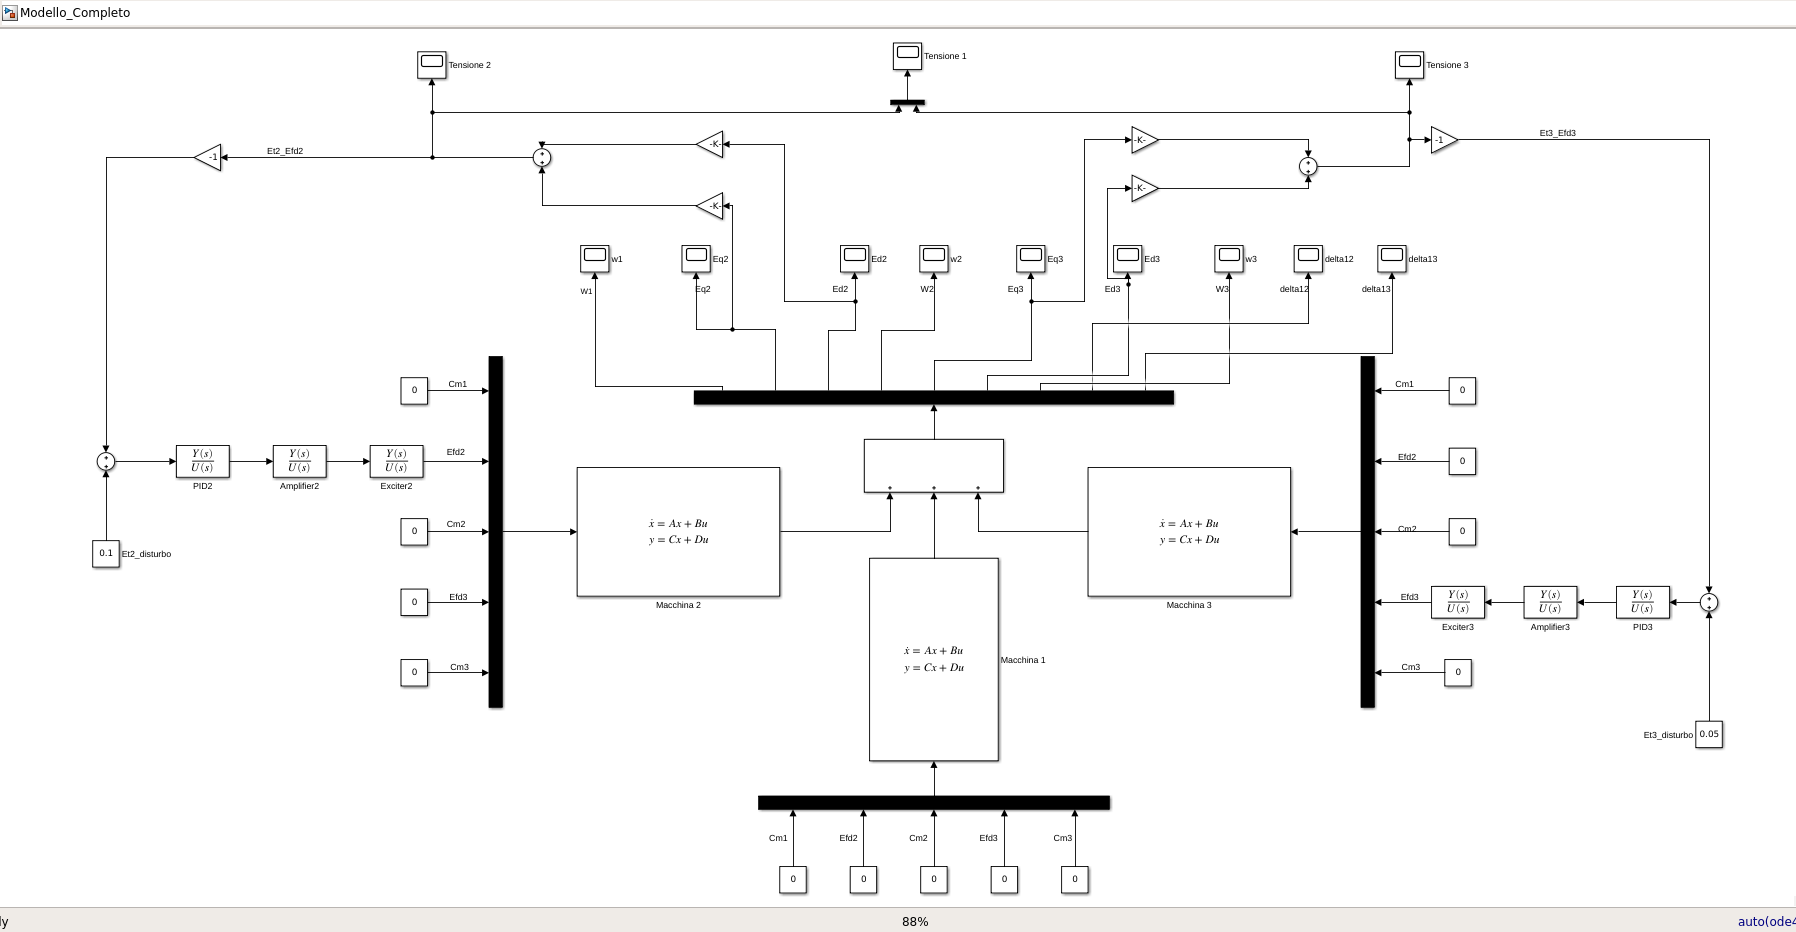
\includegraphics[scale=0.35,angle=-90]{Modello_controllato}\\
	Di seguito sono riportati più in dettaglio gli schemi dei controllori.\\\\
	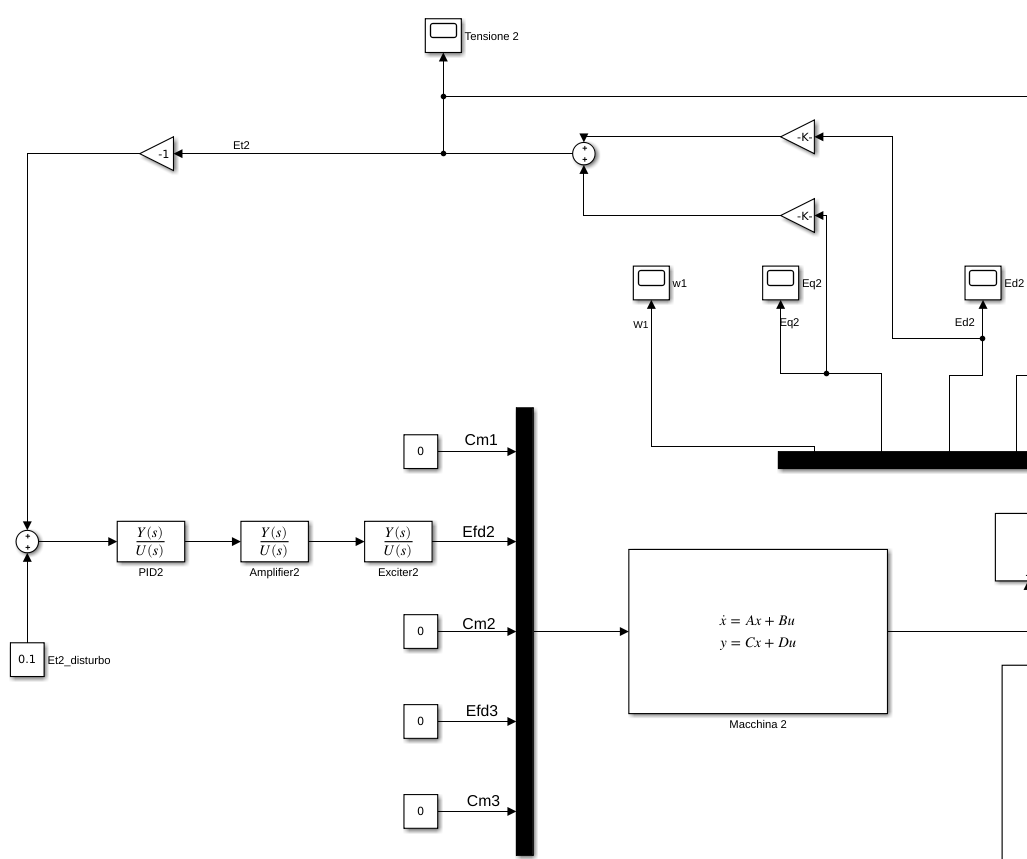
\includegraphics[scale=0.5,angle=90]{Dettaglio_controllore2}\\
	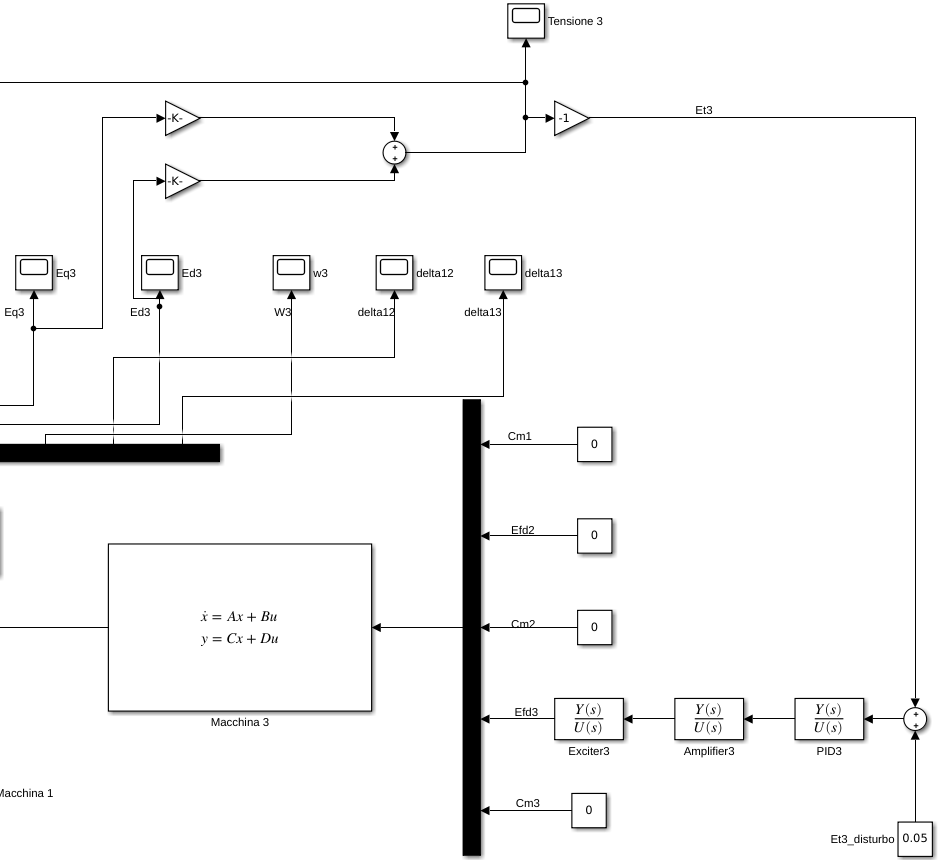
\includegraphics[scale=0.5,angle=-90]{dettaglio_controllore_3}\newpage
	\subsection{Simulazioni}
	Lo studio del sistema finora è stato effettuato considerando in maniera indipendente i controllori. Per di più il plant era costituito dalle sole funzioni di trasferimento $\frac{E_{ti}}{E_{fdi}}$, con $i=2,3$, e quindi senza considerare l' apporto sulla variazione di tensione da parte delle altre grandezze del sistema. E' possibile evincere le performance dei PID inseriti nel sistema MIMO dalle simulazioni riportate di sotto, prima nel caso di inseguimento di un riferimento, poi nel caso di disturbi.
	\begin{figure}[h]
		\centering
		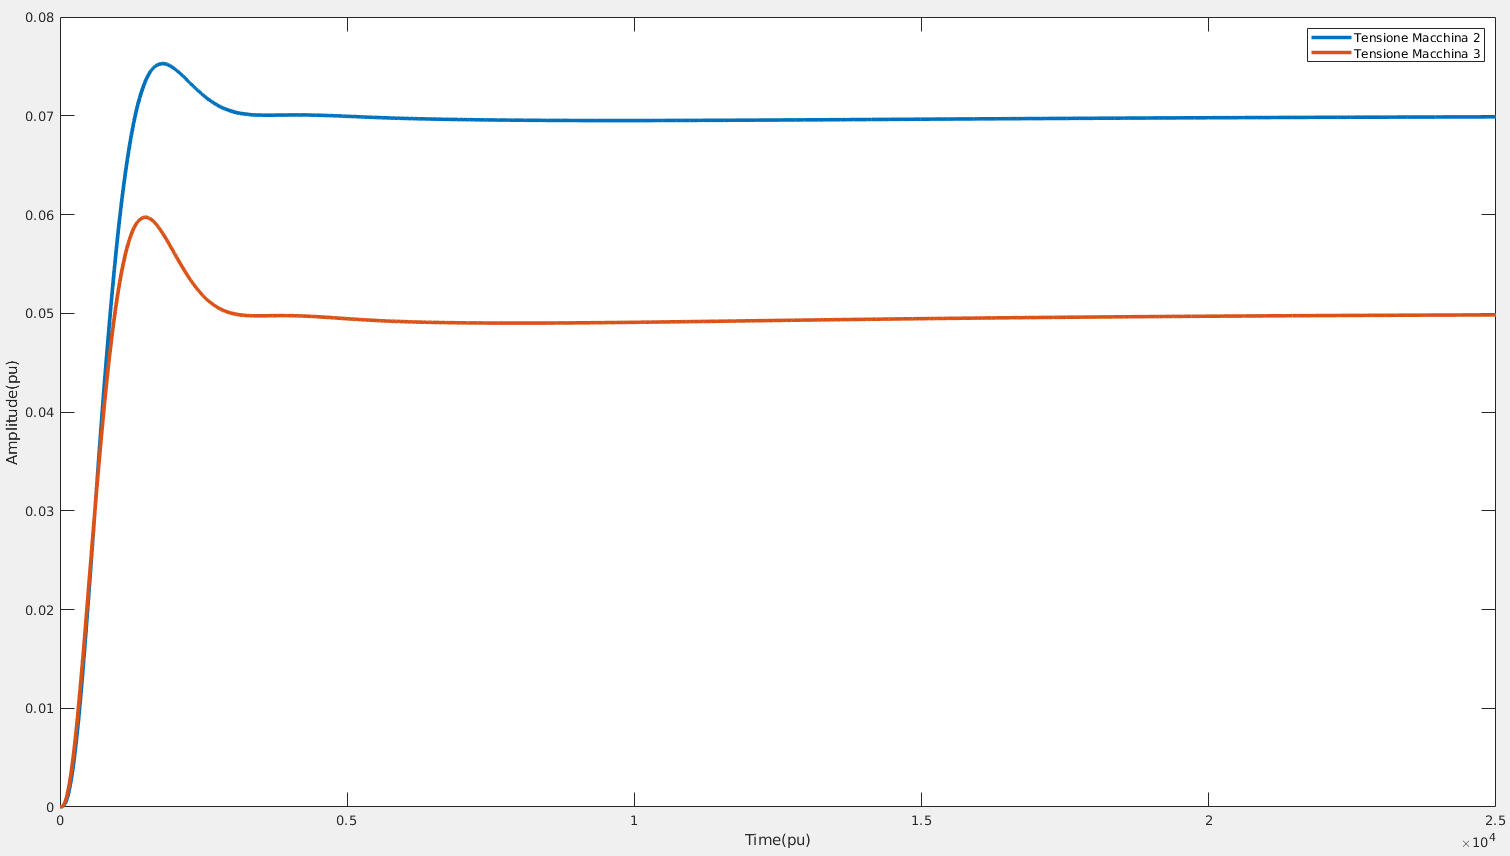
\includegraphics[scale=0.26]{simulazione_riferimento}
		\caption{Inseguimento di un riferimento di 0.07 (macchina 2) e 0.05 (macchina 3)}
		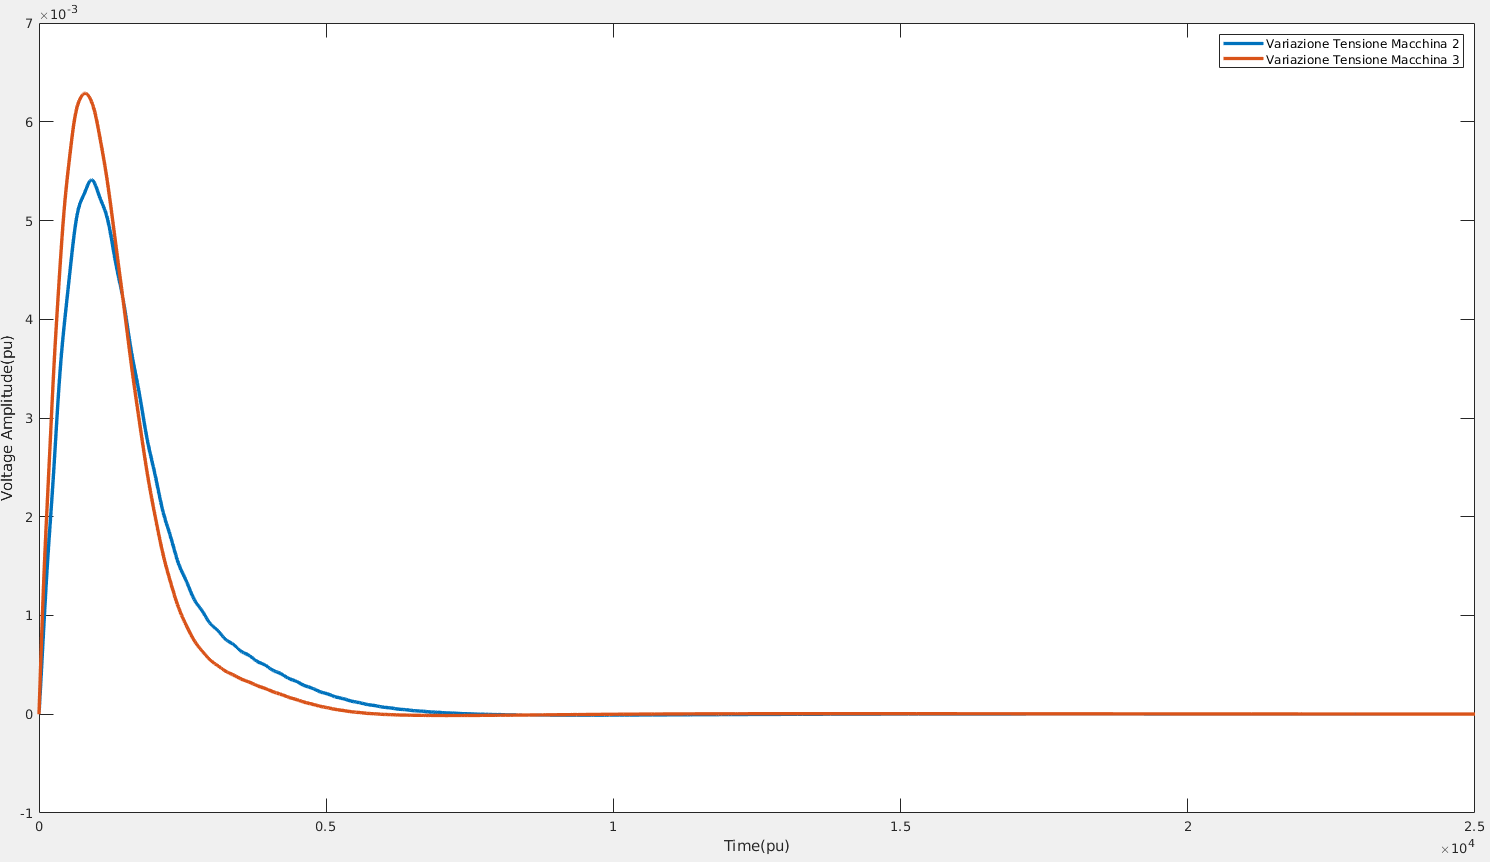
\includegraphics[scale=0.26]{simulazione_disturbo}
		\caption{Inseguimento di un disturbo di 0.03 (macchina 2) e 0.05 (macchina 3)}
	\end{figure}
	A pagina seguente vengono riportate in tabella le caratteristiche della risposta in caso di inseguimento.\\
	\begin{tabular}{|l|l|l|}
		\hline
		& \textbf{Macchina 2}	& \textbf{Macchina3}\\
		\hline
		\textbf{Rise Time} & 735.0136 pu = 1.94 s & 569.5282 pu = 1.5 s\\
		\textbf{Settling Time} & 3703 pu = 9.82 s & 4012.7 pu = 10.64 s\\
		\textbf{Overshoot} & 17.9591 & 31.4618\\
		\textbf{Undershoot} & 0 & 0\\
		\textbf{Peak} & 0.0826 & 0.0657\\
		\textbf{Peak Time} & 1775 pu = 4.7 s & 1483 pu = 3.93 s\\
		\hline	\end{tabular}\\\\
	Qui sotto invece le caratteristiche della risposta in seguito al disturbo:\\\\
	\begin{tabular}{|l|l|l|}
		\hline
		& \textbf{Macchina 2}	& \textbf{Macchina3}\\
		\hline
		\textbf{Settling Time} & 5634.2 pu = 14.9 s & 4591.8 pu = 12.17 s\\
		\textbf{Peak} & 0.0054 & 0.0063\\
		\textbf{Peak Time} & 915.5 pu = 2.4 s & 803 pu = 2.13 s\\
		\hline
	\end{tabular}\\\\
	Concentrandoci sulla simulazione nel caso di riferimento, possiamo vedere come la sovraelongazione sia elevata in entrambi i casi, e questo è dovuto alla presenza di un' azione integrale abbastanza elevata. Utilizzando lo script "migliora\textunderscore itegrale\textunderscore script.m" (appendice), è possibile modificare la costante $T_i$ dell' azione integrale lasciando inalterati gli altri parametri. Questa modifica viene fatta direttamente analizzando come si comporta l' intero sistema modellato in Simulink, impostando un valore limite del tempo d' assestamento che non si vuole oltrepassare. Nel nostro caso prenderemo come riferimento il tempo d' assestamento più elevato (4012.7 della macchina 3) e quindi imposteremo la tolleranza a 4050. Si riporta quindi la risposta del sistema dopo l' esecuzione dello script.
	\begin{figure}[h]
		\centering
		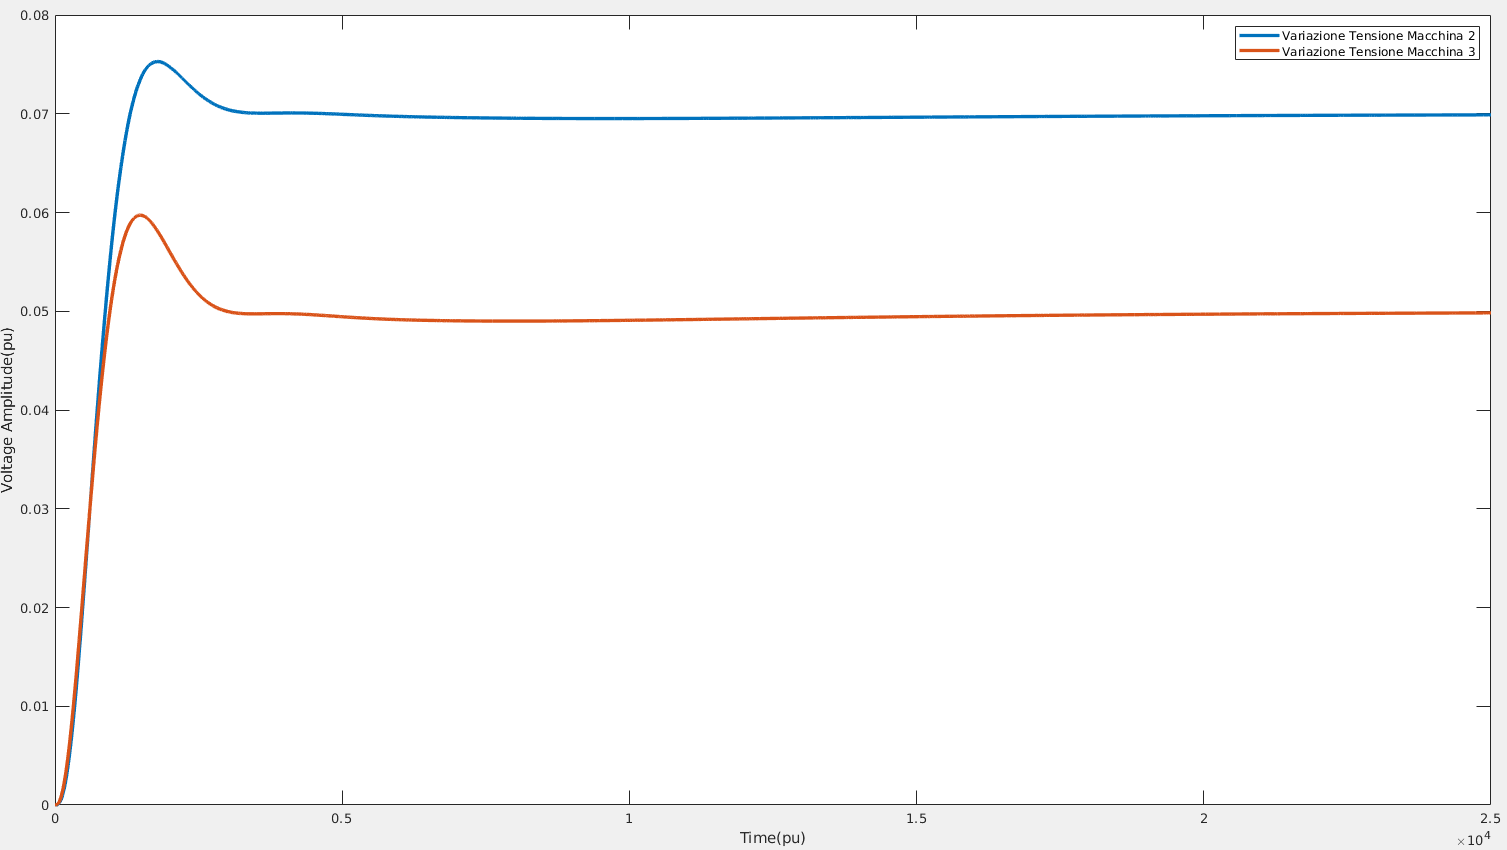
\includegraphics[scale=0.26]{simulazione_riferimento_nuovo}
		\caption{Inseguimento di un riferimento di 0.07 (macchina 2) e 0.05 (macchina 3)}
	\end{figure}
\\\\\\\\\\
	Qui di seguito invece le nuove caratteristiche nel dominio del tempo della risposta.\\\\
	\begin{tabular}{|l|l|l|}
		\hline
		& \textbf{Macchina 2}	& \textbf{Macchina3}\\
		\hline
		\textbf{Rise Time} & 819.9211 pu = 2.17 s & 620.4016 pu = 1.6 s\\
		\textbf{Settling Time} & 2650.9 pu = 7 s & 2640 pu = 7 s\\
		\textbf{Overshoot} & 7.5534 & 19.46\\
		\textbf{Undershoot} & 0 & 0\\
		\textbf{Peak} & 0.0753 & 0.0597\\
		\textbf{Peak Time} & 1792.5 pu = 4.75 s & 1485.5 pu = 3.9 s\\
		\hline
	\end{tabular}
	\subsection{Conclusioni}
	I risultati ottenuti sono soddisfacenti, ottenendo una riduzione della sovraelongazione di più del 10 percento in entrambi i casi. Anche il tempo d' assestamento è stato diminuito in maniera soddisfacente, sebbene rimanga di circa 7 secondi, che potrebbe sembrare un tempo elevato in relazione all' entità irrisoria dei disturbi.
	\begin{figure}[h]
		\centering
		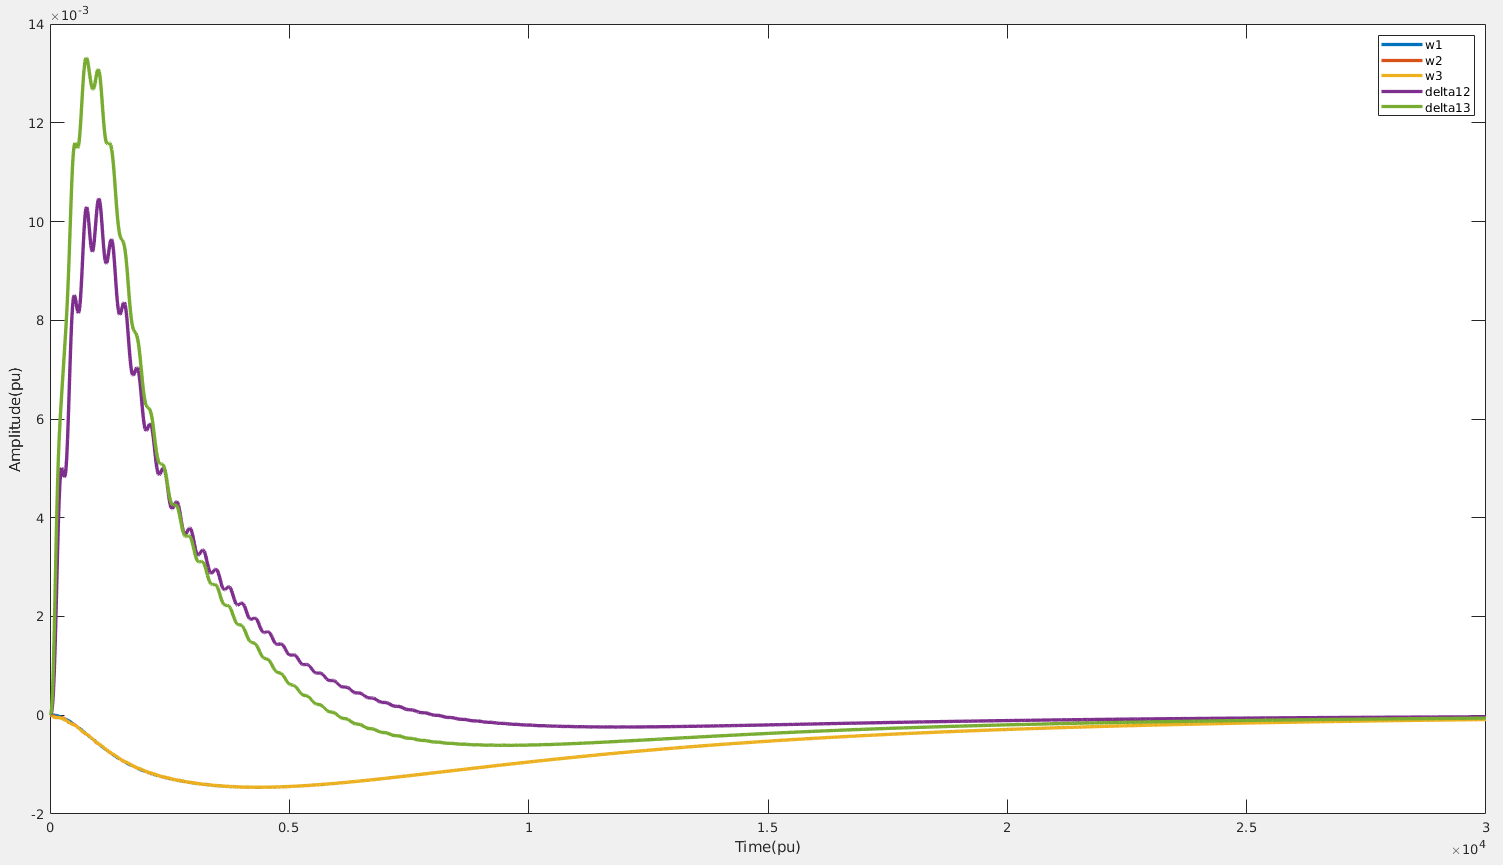
\includegraphics[scale=0.255]{simulazione_oscillazioni_disturbo}
		\caption{Andamento delle $\omega_i$ e dei $\delta_i$ in seguito all' applicazione di un disturbo}
	\end{figure}
	 Per giustificare questi risultati ci sono da fare diverse considerazioni. In primo luogo, il controllo di questo sistema MIMO è stato effettuato utilizzando un approccio SISO, analizzando la funzione di trasferimento tensione di field-tensione di output e quindi trascurando l' influsso che le altre variabili del sistema hanno sulla tensione d' uscita. Queste ultime inoltre sono lasciate incontrollate, e soprattutto le $\omega_i$ sono delle variabili che hanno una dinamica lenta come si può osservare in figura 3.10, e vanno ad influenzare la variabile controllata di interesse. Queste non vanno ad influenzare direttamente la dinamica delle tensioni, come si può constatare guardando lo spazio di stato generale del sistema interconnesso, ma intervengono direttamente nella dinamica dei vari $\delta_i$, che influenzano in maniera significativa le tensioni. Un altro aspetto da considerare è che il tuning dei controllori è stato eseguito in maniera obsoleta rispetto a quanto fanno gli algoritmi intelligenti. I parametri del PID sono stati difatti determinati offline, in maniera univoca una volta condotto lo studio, utilizzando delle regole empiriche. Inoltre i controllori non cooperano tra loro per massimizzare un obiettivo; il controllore della seconda macchina, per esempio, applica la legge di controllo senza considerare l' azione che esercita il controllore della terza macchina. Questa situazione, proprio per la natura dell' AVR, aumenta la instabilità delle $omega_i$ e di conseguenza le oscillazioni dei $delta_i$. Delle migliorie, sempre nell' ambito della small signal analysis, potrebbero essere apportate in questo senso, cioè utilizzando degli algoritmi online per il tuning del PID, costruendo magari una funzione obiettivo che riesce quindi a far lavorare più in sintonia fra loro i vari controllori.
	\appendix
	\chapter{Codici Matlab}
	Nelle pagine seguenti verranno proposti i codici Matlab (funzioni e script) che sono stati utilizzati in questo lavoro.\newpage
	\begin{figure}
		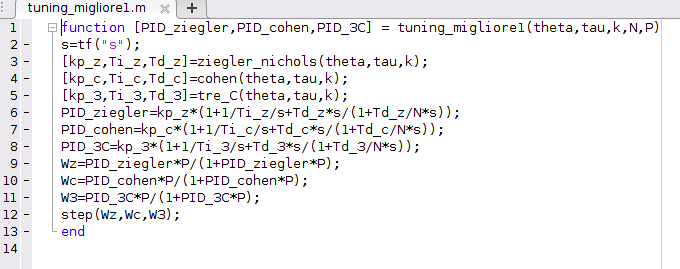
\includegraphics[scale=0.55]{tuning_migliore}
		\caption{Codice per trovare il metodo di tuning più performante}
	\end{figure}
	\begin{figure}
		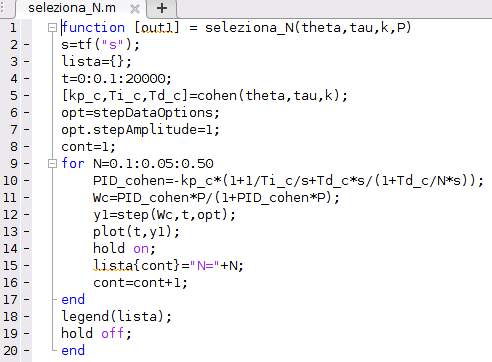
\includegraphics[scale=0.6]{seleziona_n}
		\caption{Funzione per individuare il filtro migliore per l' azione derivativa}
	\end{figure}
	\begin{figure}
	\includegraphics[scale=0.5]{tuning_selezionaN}
	\caption{Trova il migliore metodo per tempo d' assestamento al variare del filtro dell' azione derivativa}
	\end{figure}
	\begin{figure}
		\includegraphics[scale=0.5]{trova_parametri}
		\caption{Trova il valore del guadagno proporzionale e delle costanti di tempo delle azioni integrale e derivativa}
	\end{figure}
	\begin{figure}
		\includegraphics[scale=0.5,angle=90]{migliora_integrale_script}
		\caption{Aumenta la costante di tempo dell' azione integrale nell' intento di diminuire la sovraelongazione}
	\end{figure}

	\begin{thebibliography}{9}
		\bibitem{Power System Control and Stability}
		P. M. Anderson, A. A. Fouad,
		\textit{"Power System Control and Stability"}.
		Second Edition, 2003.
		
		\bibitem{Small-signal stability, control
			and dynamic performance of power systems}
			M.J. Gibbard, P. Pourbeik and D.J. Vowles,
			\textit{"Small-signal stability, control
				and dynamic performance of power systems"}.
			University of Adelaide Press,
			Adelaide, 2015.
		\bibitem{Power System Stability and Control}
		Prabha Kundur,
		\textit{"Power System Stability and Control"}. McGraw Hill
	\end{thebibliography}
	

	
	
	
	
	
	

	
\end{document}